\section{The  analysis of two Same Signed Lepton }
\label{sec:TwoLSS}

\subsection{Overview of the electron charge flip background estimation in two lepton same-sign}

Charge-flip events originite mainly from Z+jets, di-boson and $t\bar{t}$ processes. 
These events pollute $ee$ and $e\mu$ regions because of one electron having hard bremsstrahlung plus asymmetric conversion
($e^\pm \rightarrow e^\pm \gamma^* \rightarrow e^\pm e^+e^-$) or a wrongly measured track curve. Muon charge-flip is negligible in 
in the $\pT$ range relevant to this analysis. A dedicated tool to reduce electron charge flip is 
used (ref to ECID cut).

The rate of electron charge flips is measured from the data, based on the measured ratio of $Z\rightarrow e^{+}e^{-}$ that are 
reconstructed as a same-sign electron pair ($e^{+}e^{+}$ or $e^{-}e^{-}$). For
this, a likelihood-based method has been developed to provide the charge flip
rates, $\epsilon_{\textrm{mis id}}$, as a function of the electron $|\eta|$
and $\pT$, as shown in Fig.~\ref{fig:Lik2Ddata_main}. Sources of systematical
uncertainties on $\epsilon_{\textrm{mis id}}$ are summarized as follows:
\begin{itemize}
\item The statistical uncertainty from the likelihood method $\sigma_\epsilon^\mathrm{likelihood}(|\eta|,p_{\textrm T})$. 
\item The difference between rates measured with the likelihood method and truth-matching with simulated $Z\rightarrow e^+e^-$ events.
\item The variation of the rates with the definition of the dilepton invariant mass region, defining the $Z$-peak, and its sidebands which are used to subtract the contamination from non-prompt leptons.
\end{itemize}

The values of the total systematic uncertainties are shown in Fig.~\ref{fig:QMisID:systtight1} for tight and anti-tight electrons.

\begin{figure}[h!]
\centering
  {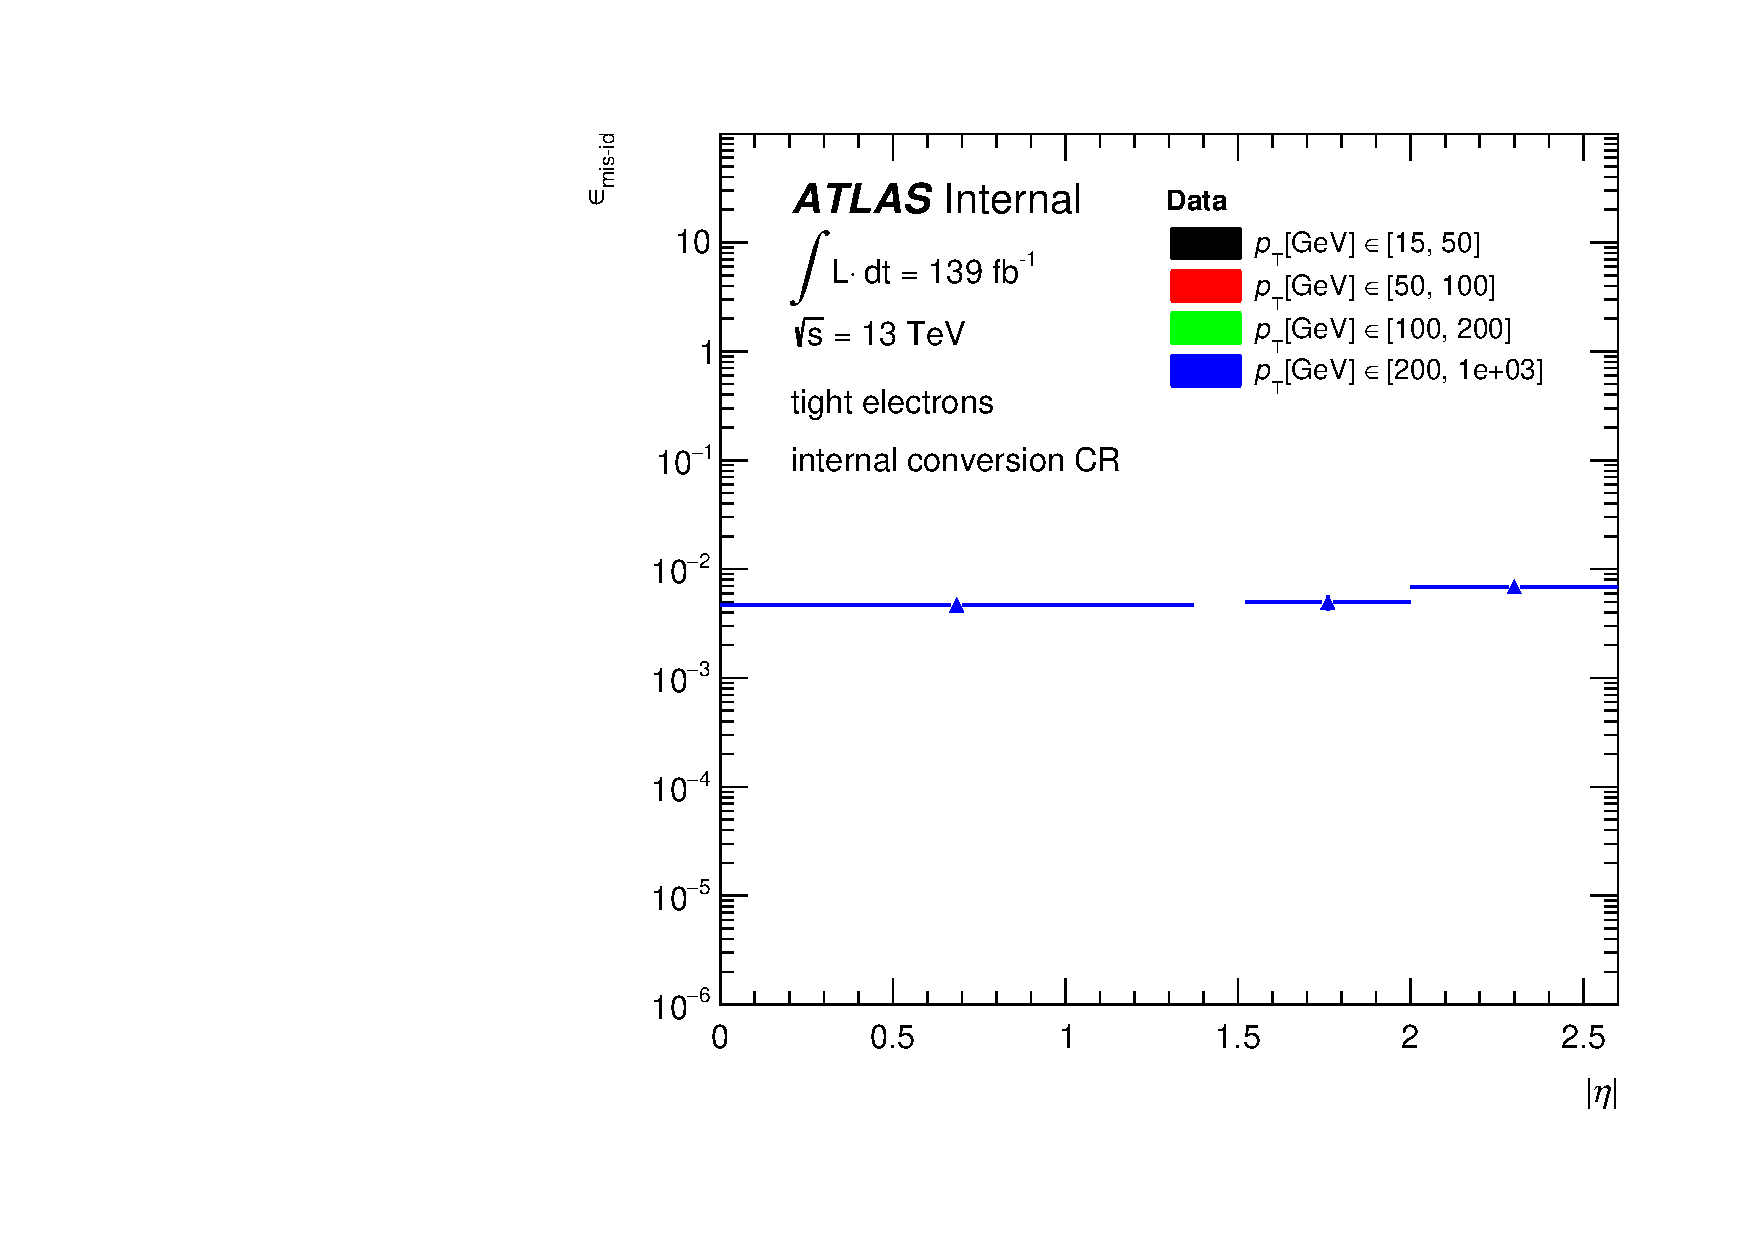
\includegraphics[width=0.32\textwidth]{figures/qmisid/crateData_tight_m0}}
  {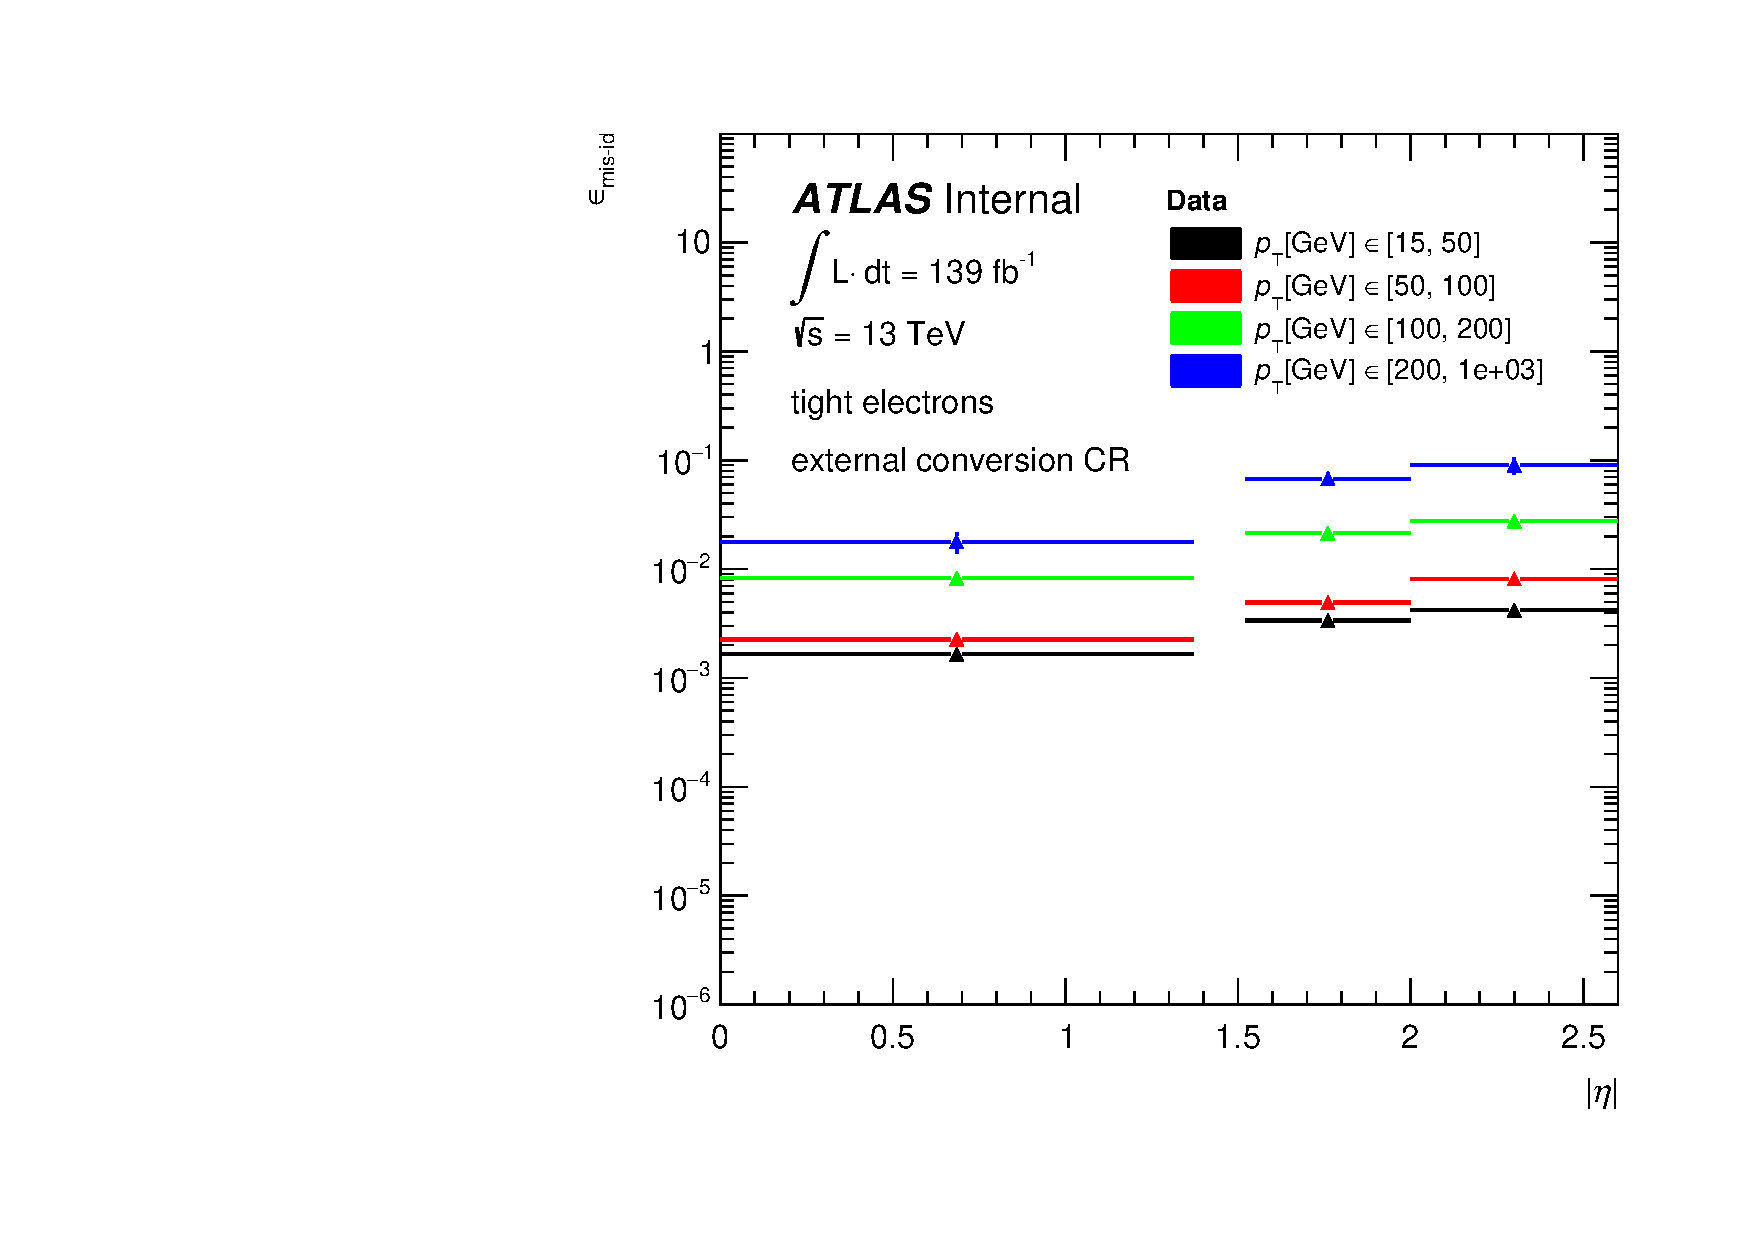
\includegraphics[width=0.32\textwidth]{figures/qmisid/crateData_tight_m1}}
  {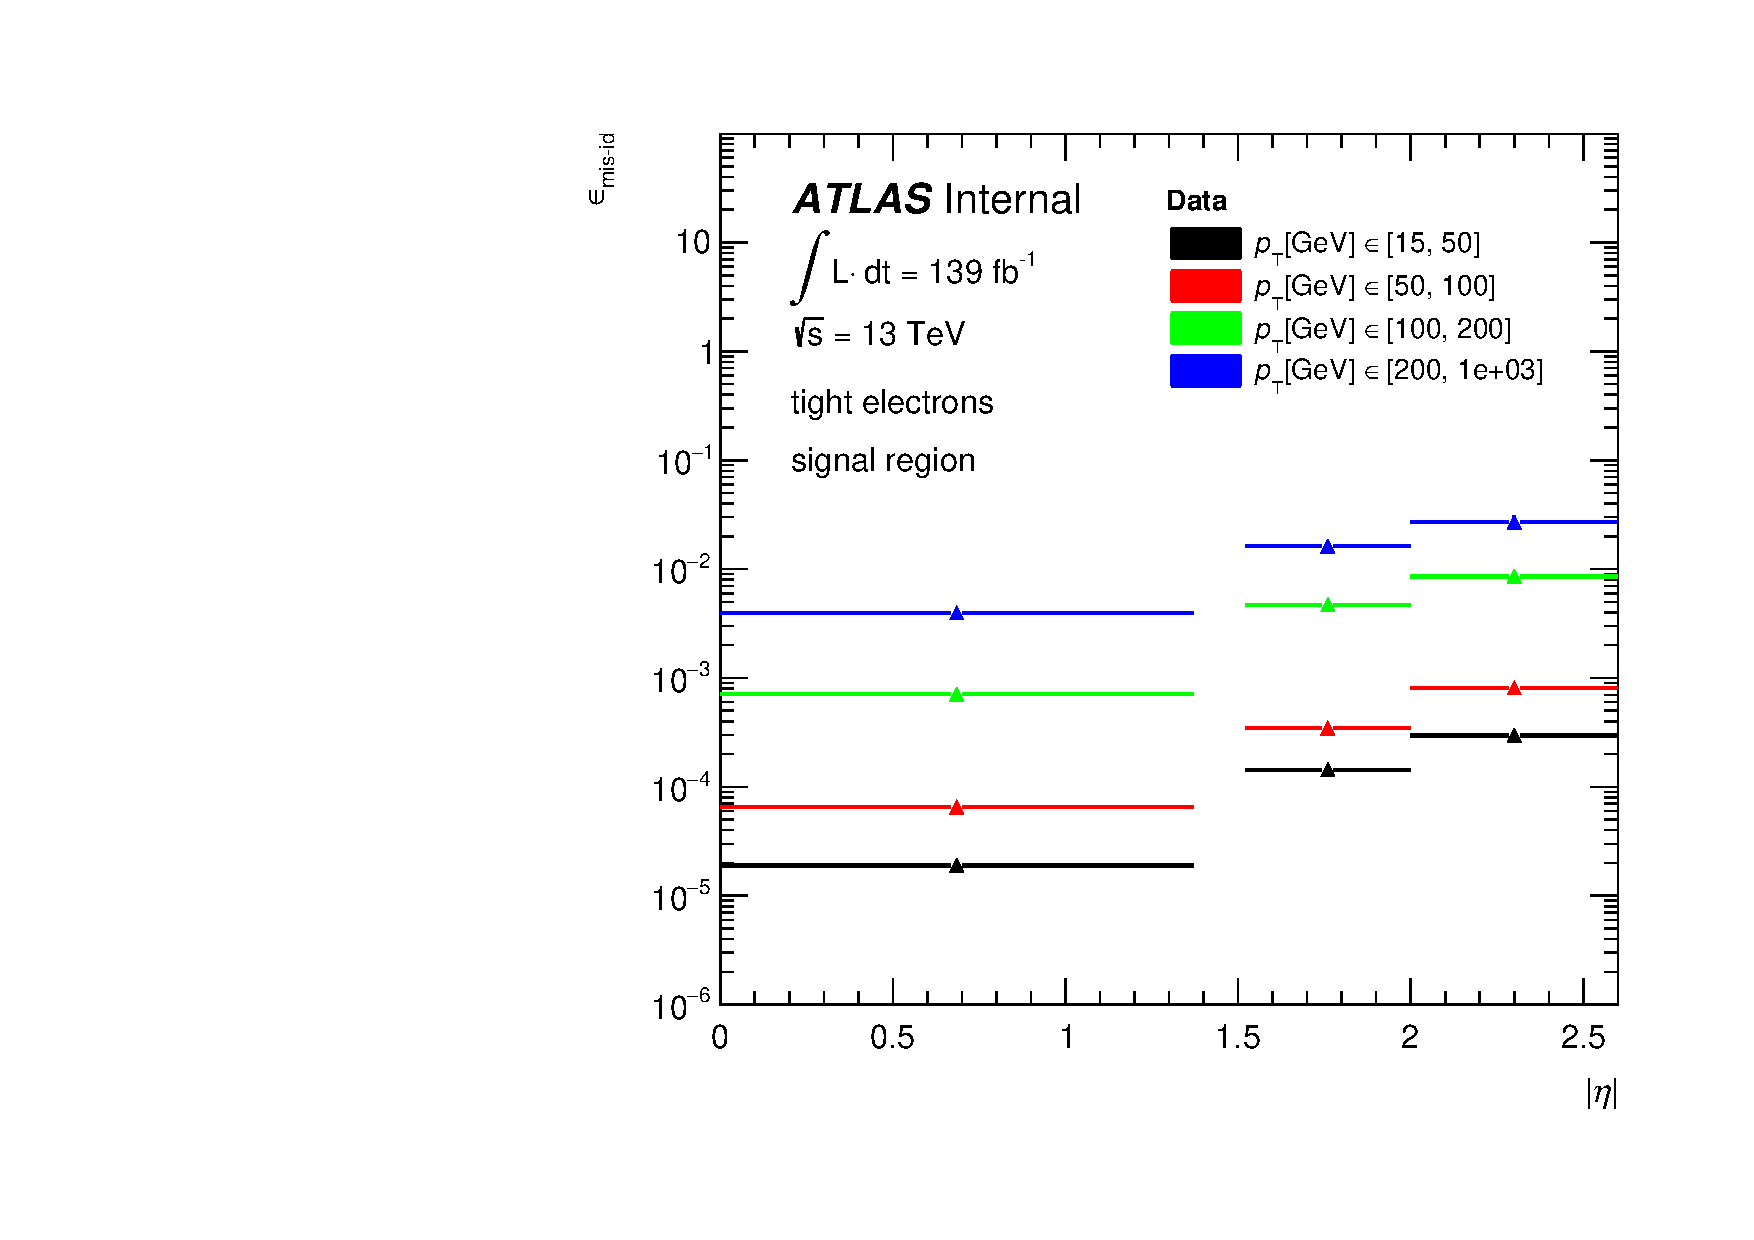
\includegraphics[width=0.32\textwidth]{figures/qmisid/crateData_tight_m2}}
  \caption{Electron charge-flip rates derived from the data with the likelihood method. The rates are presented 
           as a function of $|\eta|$, parameterised in $\pT$ for (a) internal-conversion (b) external-conversion 
           and (c) prompt candidates.\label{fig:Lik2Ddata_main}}
\end{figure}

\begin{figure}[htp!] 
  \centering
  {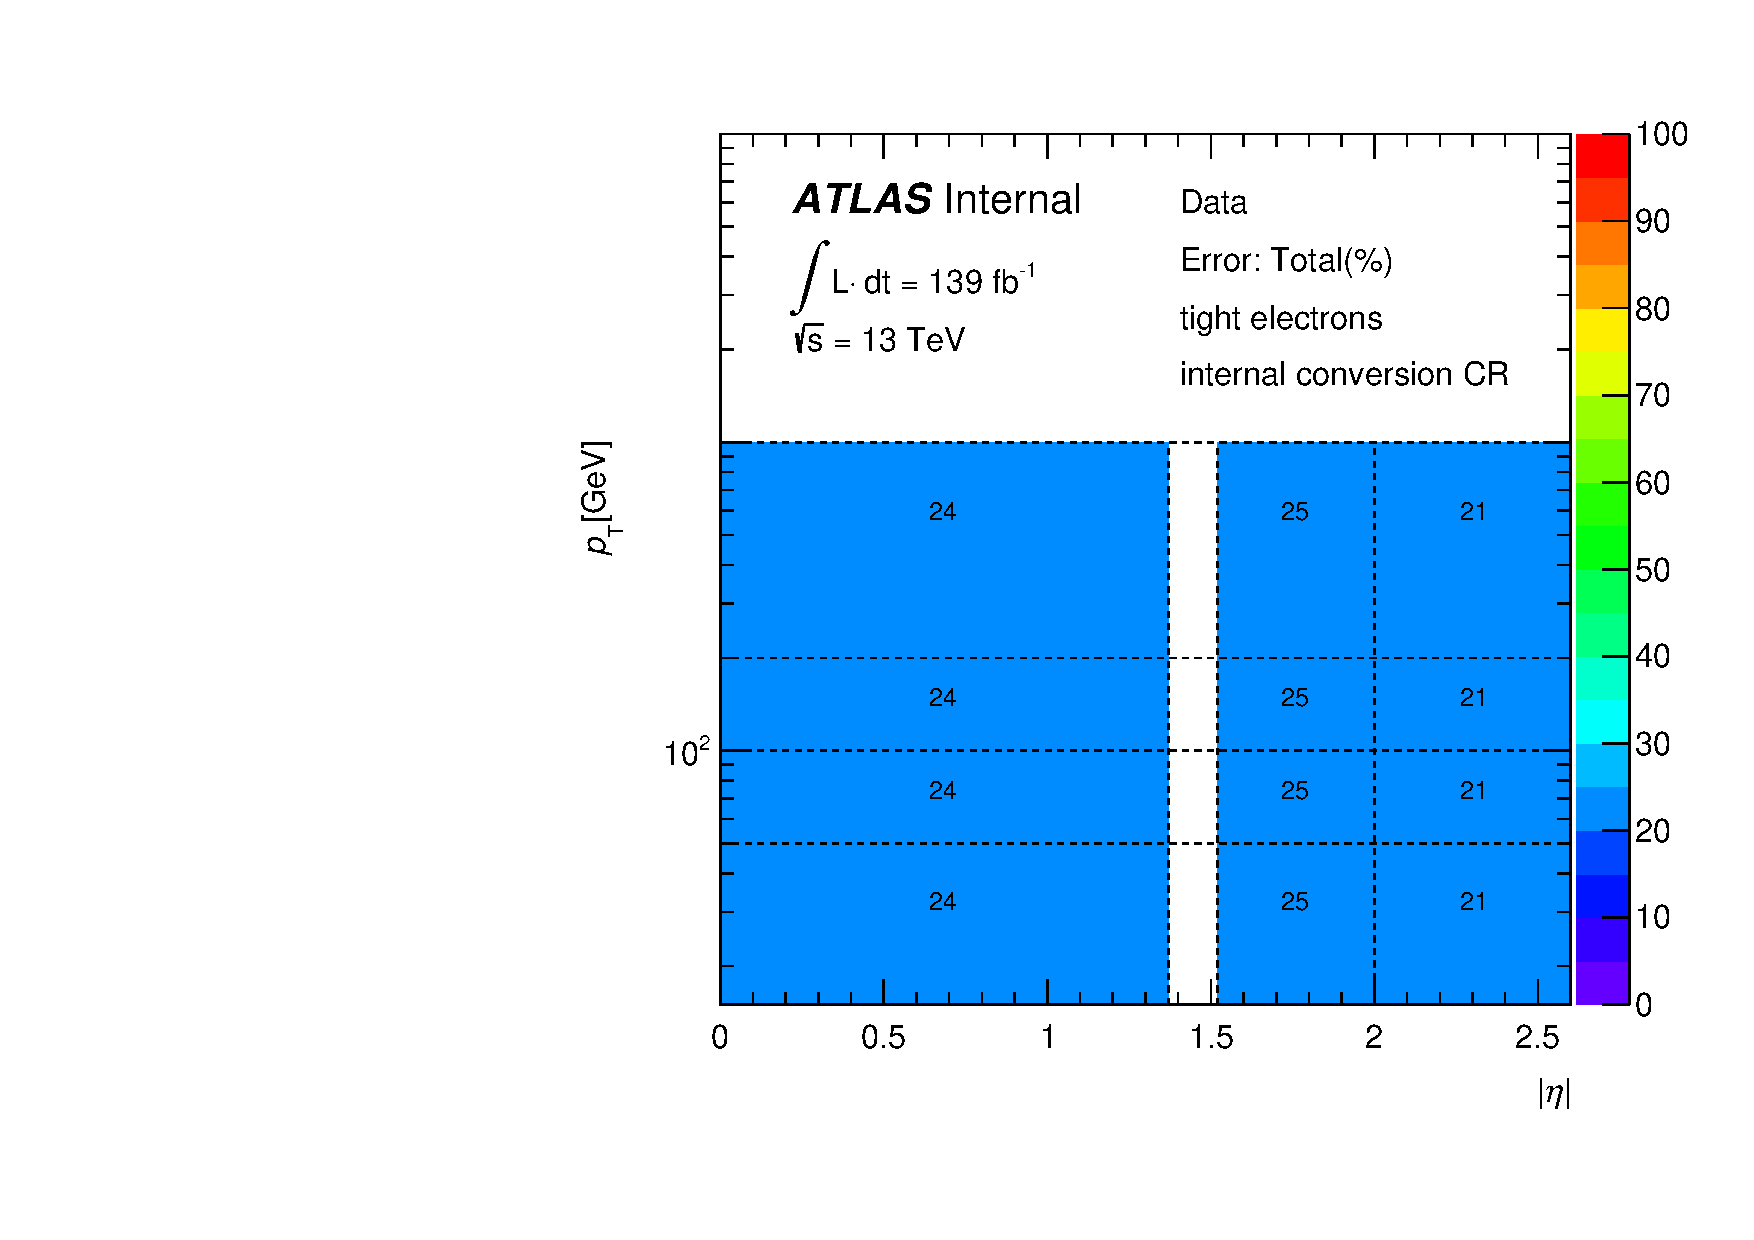
\includegraphics[width=0.32\textwidth]{figures/qmisid/syst_Data_Total_tight_intcr}}
  {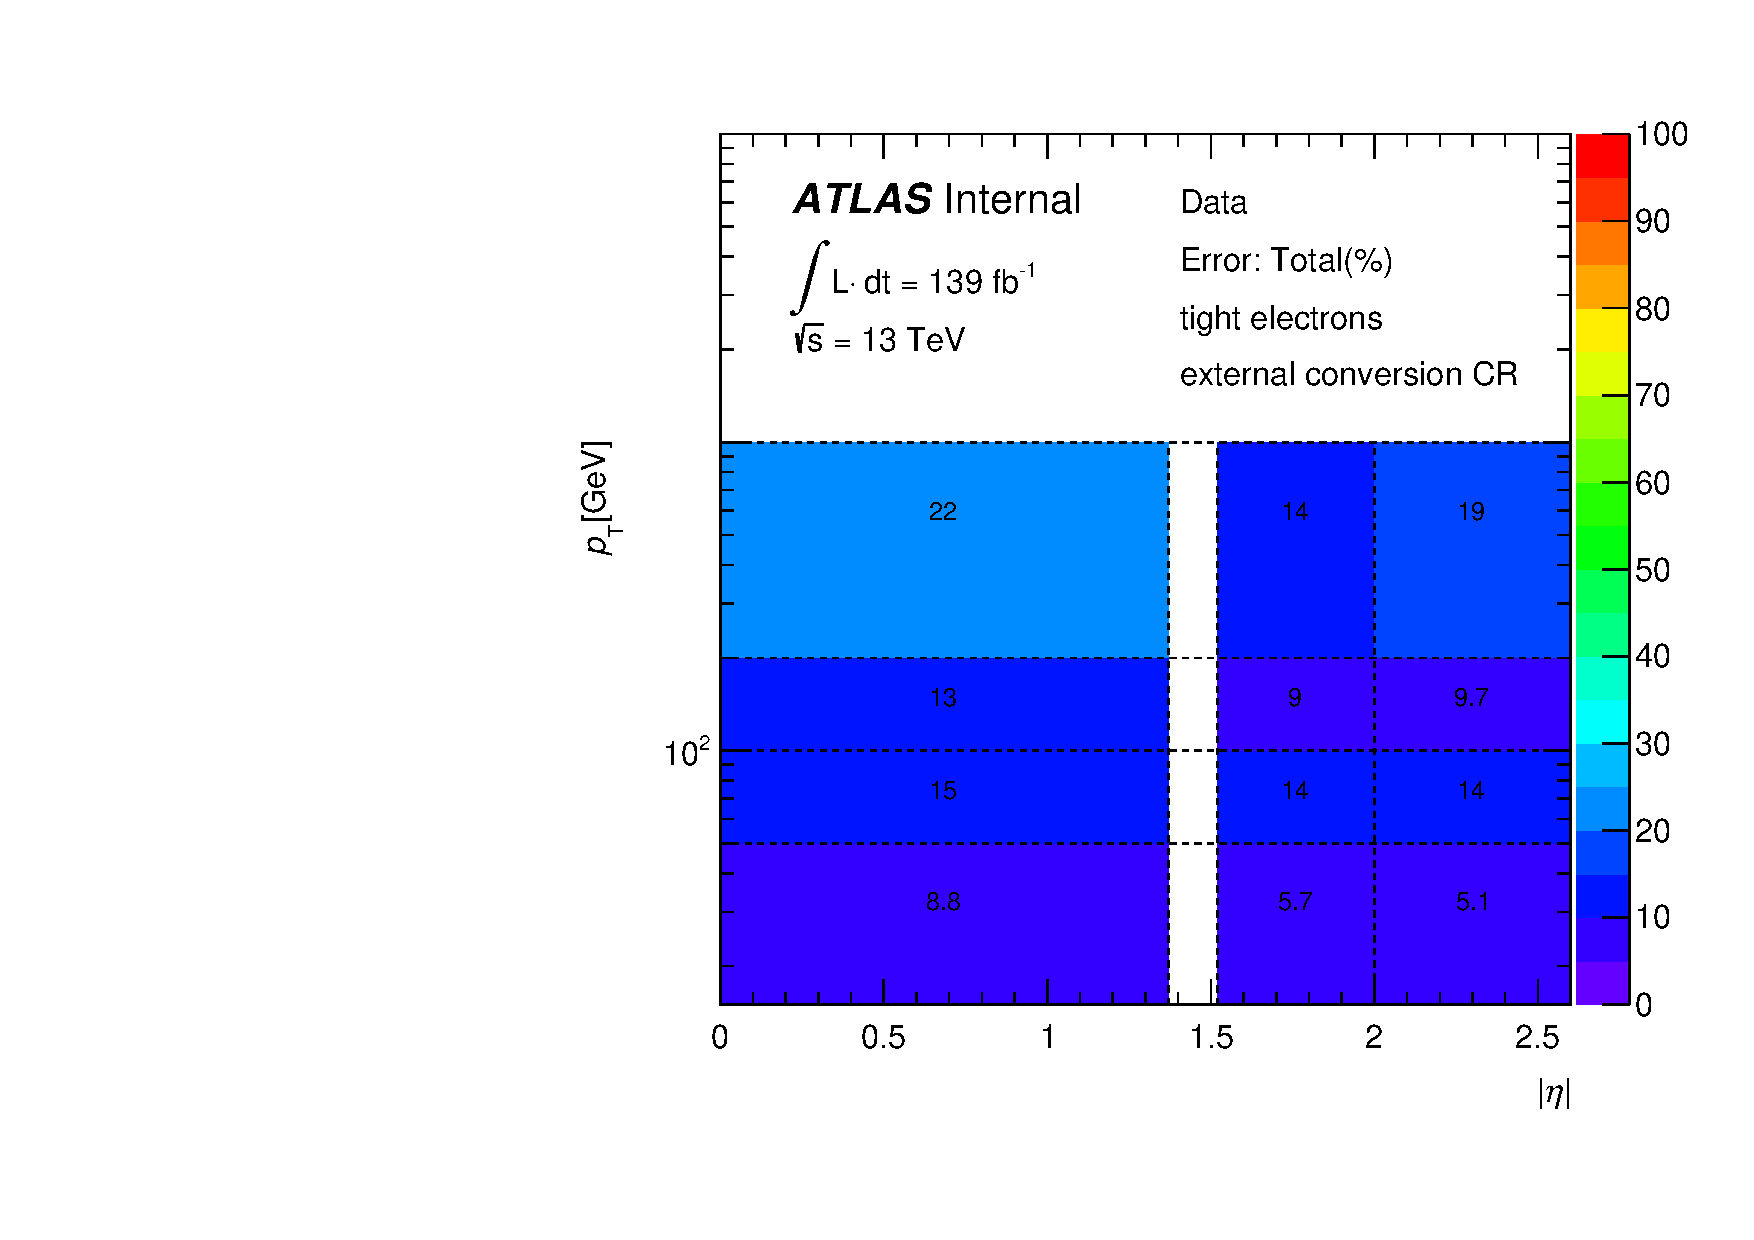
\includegraphics[width=0.32\textwidth]{figures/qmisid/syst_Data_Total_tight_extcr}}
  {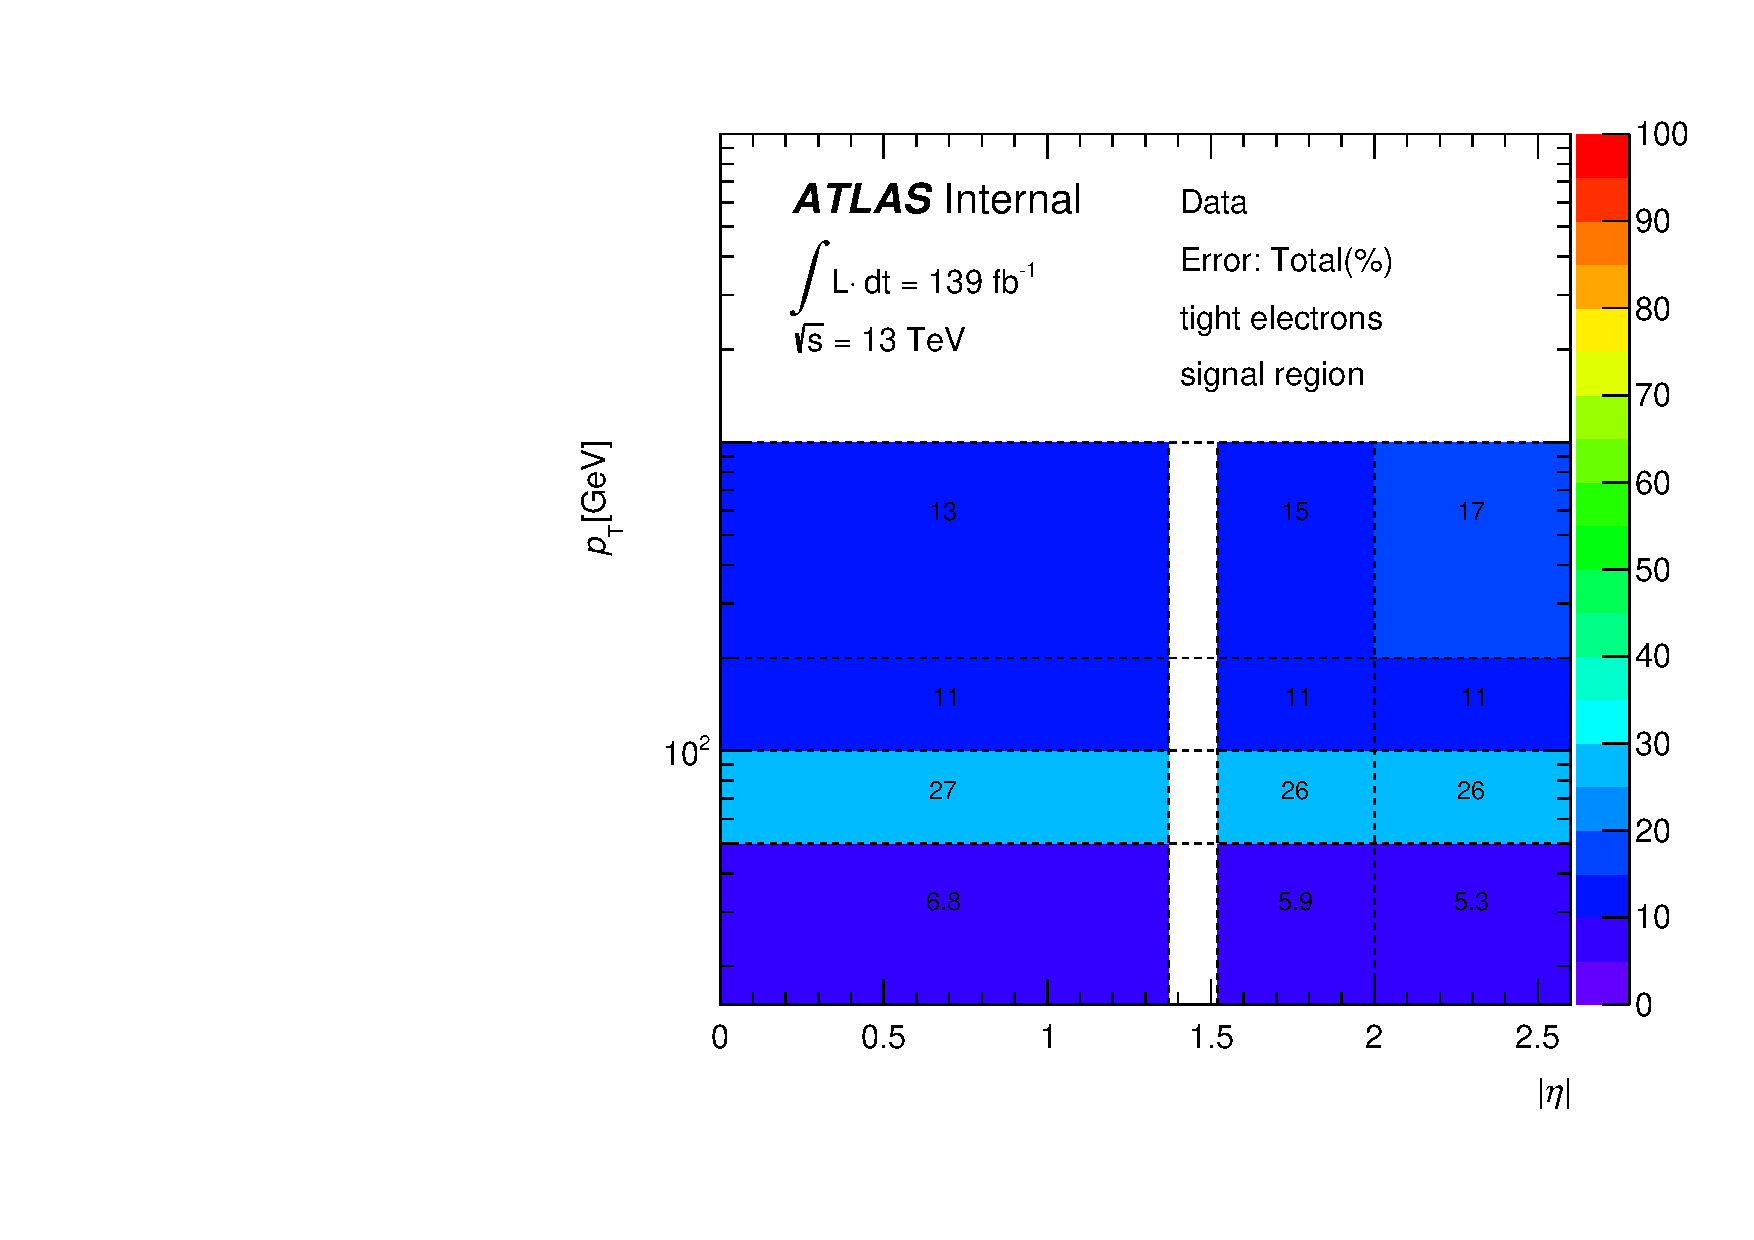
\includegraphics[width=0.32\textwidth]{figures/qmisid/syst_Data_Total_tight_sr}}
  \caption{Total relative systematic uncertainty (in \%) on the charge-flip rate in bins of $|\eta|$ and 
           $\pT$ for (a) internal-conversion (b) external-conversion and (c) prompt electron candidates.
           \label{fig:QMisID:systtight1} }
\end{figure}

Event yields with charge flip electrons are obtained by weighing pre-selected events but asking for 
opposite-sign lepton instead of same-sign. The event weights ($w_{QmisID}$) are defined as:
with the expression:
\begin{equation}
w_{QmisID} = \frac{\epsilon_{\textrm{mis id},1} + \epsilon_{\textrm{mis id},2} - 2\epsilon_{\textrm{mis id},1}\epsilon_{\textrm{mis id},2}}{1-(\epsilon_{\textrm{mis id},1} + \epsilon_{\textrm{mis id},2} - 2\epsilon_{\textrm{mis id},1}\epsilon_{\textrm{mis id},2})}
\label{eq:QmisID_weight}
\end{equation}

where $\epsilon_{\textrm{mis id},1}(1-\epsilon_{\textrm{mis
    id},2})+\epsilon_{\textrm{mis id},2}(1-\epsilon_{\textrm{mis id},1}) =
\epsilon_{\textrm{mis id},1} + \epsilon_{\textrm{mis id},2} -
2\epsilon_{\textrm{mis id},1}\epsilon_{\textrm{mis id},2}$ is the rate of
events in which exactly one electron is reconstructed with charge flip.
In order to account for the strong dependence of the rates to the $\pT$ and to
improve the modeling of the kinematical observables, $\pT$ continuous rates are used.

\subsection{Electron charge flip background study}

The following paragraphs present the measurement of the background, introduced to final states with two 
same-sign light leptons ($e^{\pm}e^{\pm}$, $e^{\pm}\mu^{\pm}$) due to electron charge misidentification 
(QMisID).\footnote{Unless specified otherwise, positrons and electrons are both called electrons.} There 
are two main mechanisms contributing to QMisID:
%
\begin{itemize}
  \item Hard Bremsstrahlung ($e^\pm \rightarrow e^\pm \gamma^* \rightarrow e^\pm e^+e^-$). In this 
  case, QMisID occurs when the EM cluster is coupled to the track of the opposite-sign electron 
  in the trident. Since the probability of this process depends on the traversed detector material, 
  dependence of the QMisID rate on $|\eta|$ is expected.
  \item Mismeasurement of the electron track-curvature. This effect is more important in the high 
  $p_{\mathrm T}$ range (smaller curvature), therefore dependence of the rate on $p_{\mathrm T}$ 
  is also expected.
\end{itemize}
%
The misidentification of the muon charge-sign is not considered in this study. It may occur by mismeasurement 
of the track curvature, however, due to the long lever arm in the muon system and the fact that the charge is 
measured both in the inner detector and the muon spectrometer, the QMisID rate is marginal.

The estimation of the QMisID background is based on the electron QMisID rates $\vec{\epsilon}$. The latter 
are derived from the data, in three-dimensional (3D) bins according to $|\eta|$, $p_{\mathrm T}$ and the 
region to which the electron belongs with respect to photon conversions, i.e. it designated as internal- 
or external-conversion candidate or as prompt lepton (as defined in the
same-sign signal region).



%~~~~~~~~~~~~~~~~~~~~~~~~~~~~~~~~~~~
\subsubsection{Background estimation strategy} 
%~~~~~~~~~~~~~~~~~~~~~~~~~~~~~~~~~~~
Final states with an opposite-sign lepton pair (mainly $Z \rightarrow e^+e^- $
followed by $t\bar{t} \rightarrow b\bar{b}W^+W^- \rightarrow b\bar{b}e^+e^-\nu\bar{\nu}$)
contaminate the signal region, defined by two same-sign leptons, when the charge of exactly one lepton
is misidentified. In the case of $e^{-}e^{+}$, the fraction of events that are reconstructed as same-sign 
($e^{-}e^{-}$ or $e^{+}e^{+}$) is:
%
\begin{equation}
  \epsilon_i(1-\epsilon_j) + \epsilon_j(1-\epsilon_i) = \epsilon_i +\epsilon_j - 2\epsilon_i\epsilon_j, 
\end{equation}
%
where $\epsilon_i$ and $\epsilon_j$ are the QMisID rates for each of the two electrons. For $e^{\pm}\mu^{\mp}$ 
events, on the other hand, the respective fraction is equal to the QMisID rate $\epsilon_i$ of the electron. 
By knowing the QMisID rates it is thereby possible to compute the expected number of misidentified same-sign 
events $\bar{N}_\mathrm{SS}$ from the observed number of opposite-sign events $N_\mathrm{OS}$, using the expressions:
%
\begin{equation}
  \bar{N}_\mathrm{SS} = \frac{\epsilon_i +\epsilon_j -2\epsilon_i \epsilon_j}{1-(\epsilon_i +\epsilon_j -2\epsilon_i \epsilon_j)} N_\mathrm{OS}
  \hspace{10pt}\text{and}\hspace{10pt}
  \bar{N}_\mathrm{SS} = \frac{\epsilon_i}{1-\epsilon_i} N_\mathrm{OS}
\end{equation}
%
for the $ee$ and $e\mu$ channel, respectively.

%~~~~~~~~~~~~~~~~~~~~~~~~~~~~~~~~~~~
\subsubsection{Estimation of the charge mis-identification rates with the likelihood method} 
%~~~~~~~~~~~~~~~~~~~~~~~~~~~~~~~~~~~
The QMisID rates are derived from the data, based on the fraction of $Z\rightarrow ee$ decays that are reconstructed 
as a same-sign electron pair. For this measurement, events in the $m_{ee}$ region around the reconstructed $Z$-boson 
peak $m_Z$ are used. For $N^{ij}$ electron pairs falling in the bin combination $i,j$ (where each of $i,j$ uniquely 
represents a 3D bin as defined above) the expected number of same-sign events is:
%
\begin{equation}
  \label{app:eq:qmisid1}
  \bar{N}^{ij}_\mathrm{SS}(\epsilon_i,\epsilon_j)=N^{ij}\cdot(\epsilon_i+\epsilon_j-2\epsilon_i\epsilon_j).
\end{equation}
%
Asumming that all of the observed same-sign events, $N^{ij}_\mathrm{SS}$, in the $m_Z$ window are products 
of electron charge mis-identification, they follow a Poisson distribution around the expectation value:
%
\begin{equation}
\label{app:eq:qmisid2}
  f(N^{ij}_\mathrm{SS}|\bar{N}_\mathrm{SS}(\epsilon_i,\epsilon_j))=\frac{[{\bar{N}}^{ij}_\mathrm{SS}]^{N^{ij}_\mathrm{SS}} e^{-{\bar{N}}^{ij}_\mathrm{SS}}}{N^{ij}_\mathrm{SS}!}.
\end{equation}

which is integrated into a likelihood:
%
\begin{equation}
  L(\vec{\epsilon}|N_\mathrm{SS})=\prod_{i,j}f(N^{ij}_\mathrm{SS}|\bar{N}_\mathrm{SS}(\epsilon_i,\epsilon_j)).
\end{equation}
%
that can be maximised (minimisation of $-2\ln L$) to obtain the rates that best describe the data. 

As mentioned above, this method relies on the assumption that $ee$ events in the $m_Z$ window are products of $Z$-boson decays. 
Therefore, any contribution from other processes (e.g. fake electrons) to $N^{ij}_\mathrm{SS}$ must be subtracted. As long as 
these processes do not exhibit a resonant-like behaviour of the $m_{ee}$ distribution, this background can be estimated from 
the sidebands of the $m_{Z}$ window, for each bin combination $i,j$, separately for same-sign ($N^{ij}_\mathrm{SS,BG}$) and 
opposite-sign ($N^{ij}_\mathrm{OS,BG}$) events. For this, upper and lower sidebands are defined with width equal to the $m_{Z}$ 
window so that the introduced background can be obtained from the average yield. The background estimate is then used to correct 
the expectation (equation\,\ref{app:eq:qmisid1}) to:
%
\begin{equation}
  \bar{N}^{ij}_\mathrm{SS} = N^{ij}_\mathrm{SS,BG} + (N^{ij}-N^{ij}_\mathrm{SS,BG}-N^{ij}_\mathrm{OS,BG})\cdot(\epsilon_i+\epsilon_j-2\epsilon_i\epsilon_j).
\end{equation}
%
The minimisation of $-2\ln L$ is finally performed by MIGRAD, while HESSE is called to evaluate the uncertainty on the 
rate estimates. 

%~~~~~~~~~~~~~~~~~~~~~~~~~~~~~~~~~~~
\subsubsection{Data and Monte Carlo samples}
\label{sec:qmisiddata}
%~~~~~~~~~~~~~~~~~~~~~~~~~~~~~~~~~~~

The QMisID rate and background estimation is performed using the full dataset, with an integrated luminosity 
of 139\,fb$^{-1}$. For the validation of the method and many of the tests that follow, 
simulated $Z\to ee$ ({\scshape Sherpa}), $t\bar{t}$ (\textsc{Powheg-BOX}) and $t\bar{t}\gamma$ (\textsc{MG5\_aMC}) samples 
are also used.

No additional criteria are applied to electrons for the QMisID rate
estimation. In order to increase the size of the tight electron sample,
anti-tight electrons are also exploited.  
The latter are defined as those electrons that fail the tight identification criteria but yet pass the overlap removal. Although such 
electrons are not used in the analysis, by using a looser set of electrons and classifying them as tight and anti-tight (on top of the 
3D classification described above), introduces events with one tight and one anti-tight electron in the rate estimation, and therefore 
improves the statistical precision of the tight-electron rates with the likelihood method.

%~~~~~~~~~~~~~~~~~~~~~~~~~~~~~~~~~~~~~~~~~~~~~~~~~~~~~~~~~~~~~~~~~~~~~~~~~~
\subsubsection{$M_{ee}$ sidebands for $Z\rightarrow ee$ background estimation}
\label{app:sec:AppQMisIDregions}
%~~~~~~~~~~~~~~~~~~~~~~~~~~~~~~~~~~~~~~~~~~~~~~~~~~~~~~~~~~~~~~~~~~~~~~~~~~

The likelihood method uses $Z\rightarrow ee$ decays with both same-sign and opposite-sign electrons in the final state. As shown 
in figure\,\ref{fig:mlldata}, the $m_{ee}$ distribution of same-sign electrons is shifted towards lower values with respect to 
that of opposite-sign electrons, due to the loss of electron momentum in tridents. To account for this shift, a different $m_Z$ 
window is defined for each case. The $m_Z$ window is determined by gaussian fit around the peak (using all loose electrons) and 
defined as $\pm 4\sigma$ around the mean ($4\sigma$ has been found to provide the best results in terms of closure). The side-bands 
are defined with equal width to the $m_Z$ window, i.e. $8\sigma$ each. The region definitions are summarised in table~\ref{tab:QMisID:Ranges}.
The variation of the rates with the definition of the $m_Z$ window ($\pm 1\sigma$) is considered as a systematic uncertainty.

\smallskip

\begin{table}[h!]
  \begin{center}
    \begin{tabular}{l c c c}
      Sample & lower SB & $m_Z$ window & upper SB \\
      Same-sign & [51.7,76.5] & [76.5,101.3] & [101.3,126.0] \\
      Opposite-sign & [54.7,78.5] & [78.5,102.3] & [102.3,126.0] \\
    \end{tabular}
     \caption{Definition of the $m_Z$ window and side-bands (SB) used in the likelihood method.\label{tab:QMisID:Ranges}}
  \end{center}
\vspace*{-\baselineskip}
\end{table}

\begin{figure}[h!]
  \centering
  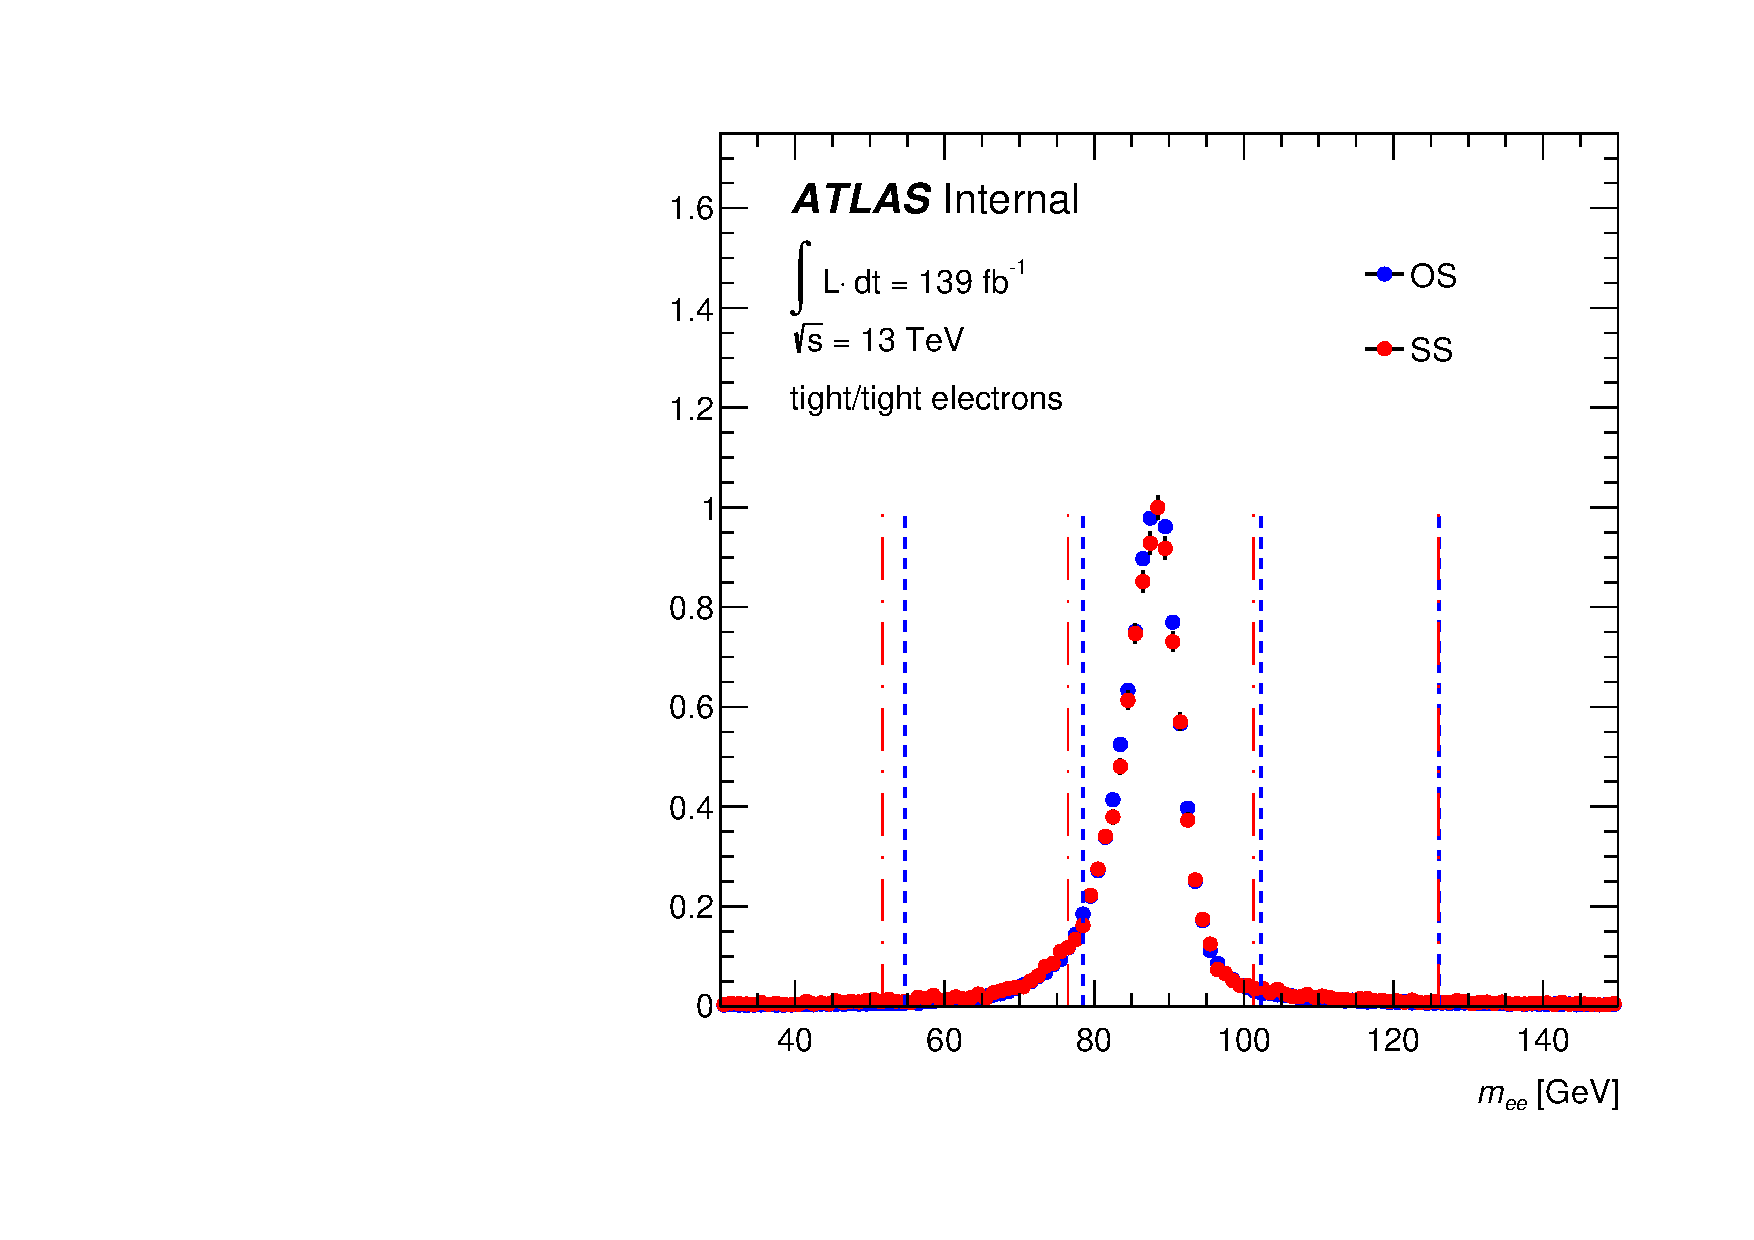
\includegraphics[width=0.45\textwidth]{figures/qmisid/mll_tt}
  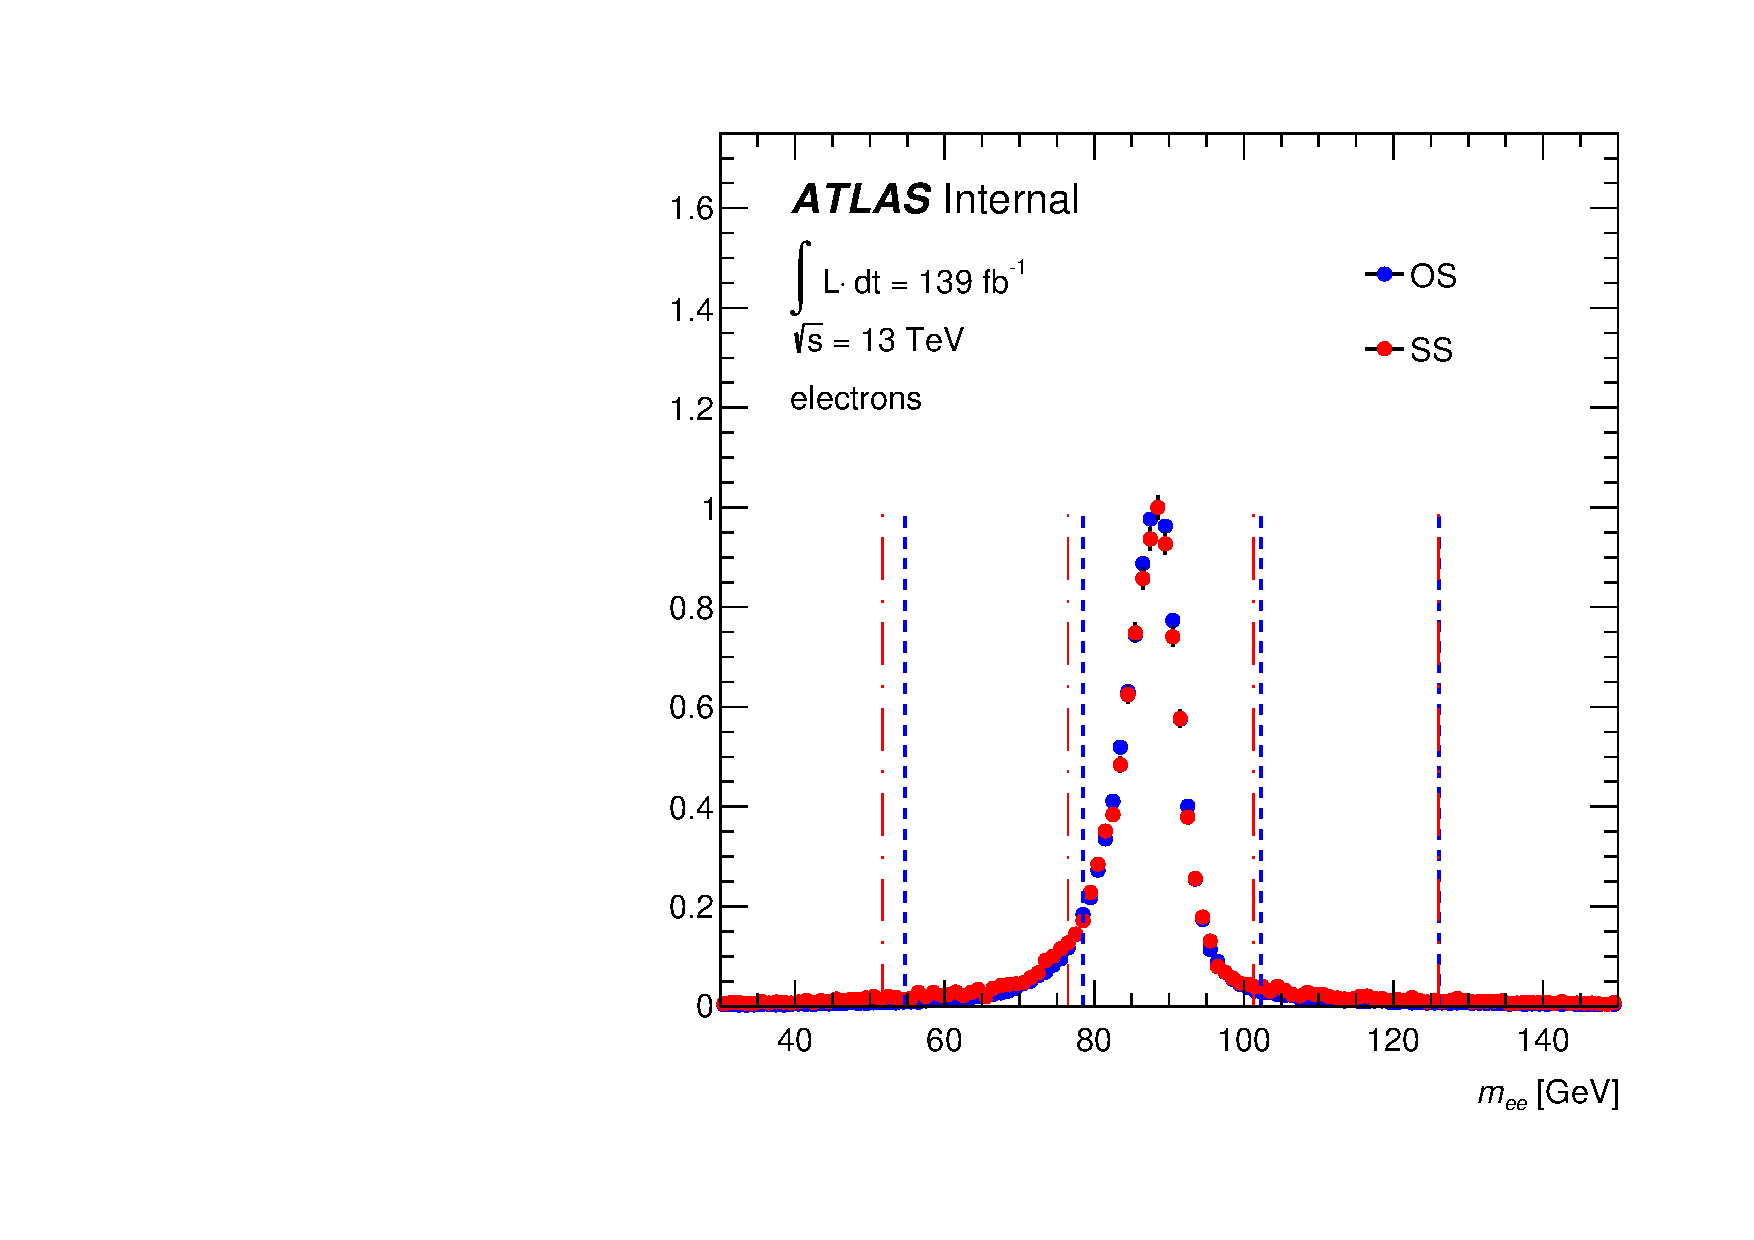
\includegraphics[width=0.45\textwidth]{figures/qmisid/mll_all}
  \caption{Comparison of the $m_{ee}$ distribution between same-sign and opposite-sign data events for pairs of 
  (a) tight and (b) loose electrons. The distributions are 
  normalized by the maximum value. The peak for same-sign electrons is shifted with respect to opposite-sign 
  electrons due to the loss of electron momentum in tridents.\label{fig:mlldata}}
\end{figure}

%~~~~~~~~~~~~~~~~~~~~~~~~~~~~~~~~~~~~~~~~~~~~~~~~~~~~~~~~~~~~~~~~~
\subsubsection{Data-driven rates estimates with $\pT$ continuous rates}
%~~~~~~~~~~~~~~~~~~~~~~~~~~~~~~~~~~~~~~~~~~~~~~~~~~~~~~~~~~~~~~~~~

The binning in $|\eta|$ and $\pT$ must be optimised to best describe the dependence of the rates on each quantity
while maintaing statistical precision.

The binning scheme 
distinguishes four bins in $|\eta|$ 
(one of which just isolates the crack region) and four bins in $\pT$, for each region w.r.t. to photon conversions. 
To mitigate the statistical uncertainties introduced by the size of the available dataset in the case of 
tight-electrons, $\pT$ bins are merged in the case of the internal conversion control region (merging is 
implemented by assigning the same rate in the likelihood).
The data-driven QMisID rates, derived with the above binning configuration, are presented in figure\,\ref{fig:Lik2Ddata}.

Figure\,\ref{fig:DatapTJumps}(a) shows the expected $\pT$ distribution in the
data, using reweighted opposite-sign events, compared to the
observation. Significant non closures are observed at the edges of the $\pT$
bins. These non-closures are covered by the non-closure systematic
uncertainties in average only. The local non-closures exceed significantly the
systematic uncertainties. They can of $200\%$ in the 60-80~GeV range, and higher
than $200\%$ in the 150-200~GeV ranges.
 
In order to control this effect, $\pT$ continuous modeling of the rates is
used. The effective rate at a given $\pT$ is obtained by the weighted
sum of the rates from the adjacend $\pT$ bins. The weighting is based on
$\pT$ only and accounts for the $\pT$ disctribution shape.

\begin{figure}[htb!]
\centering
  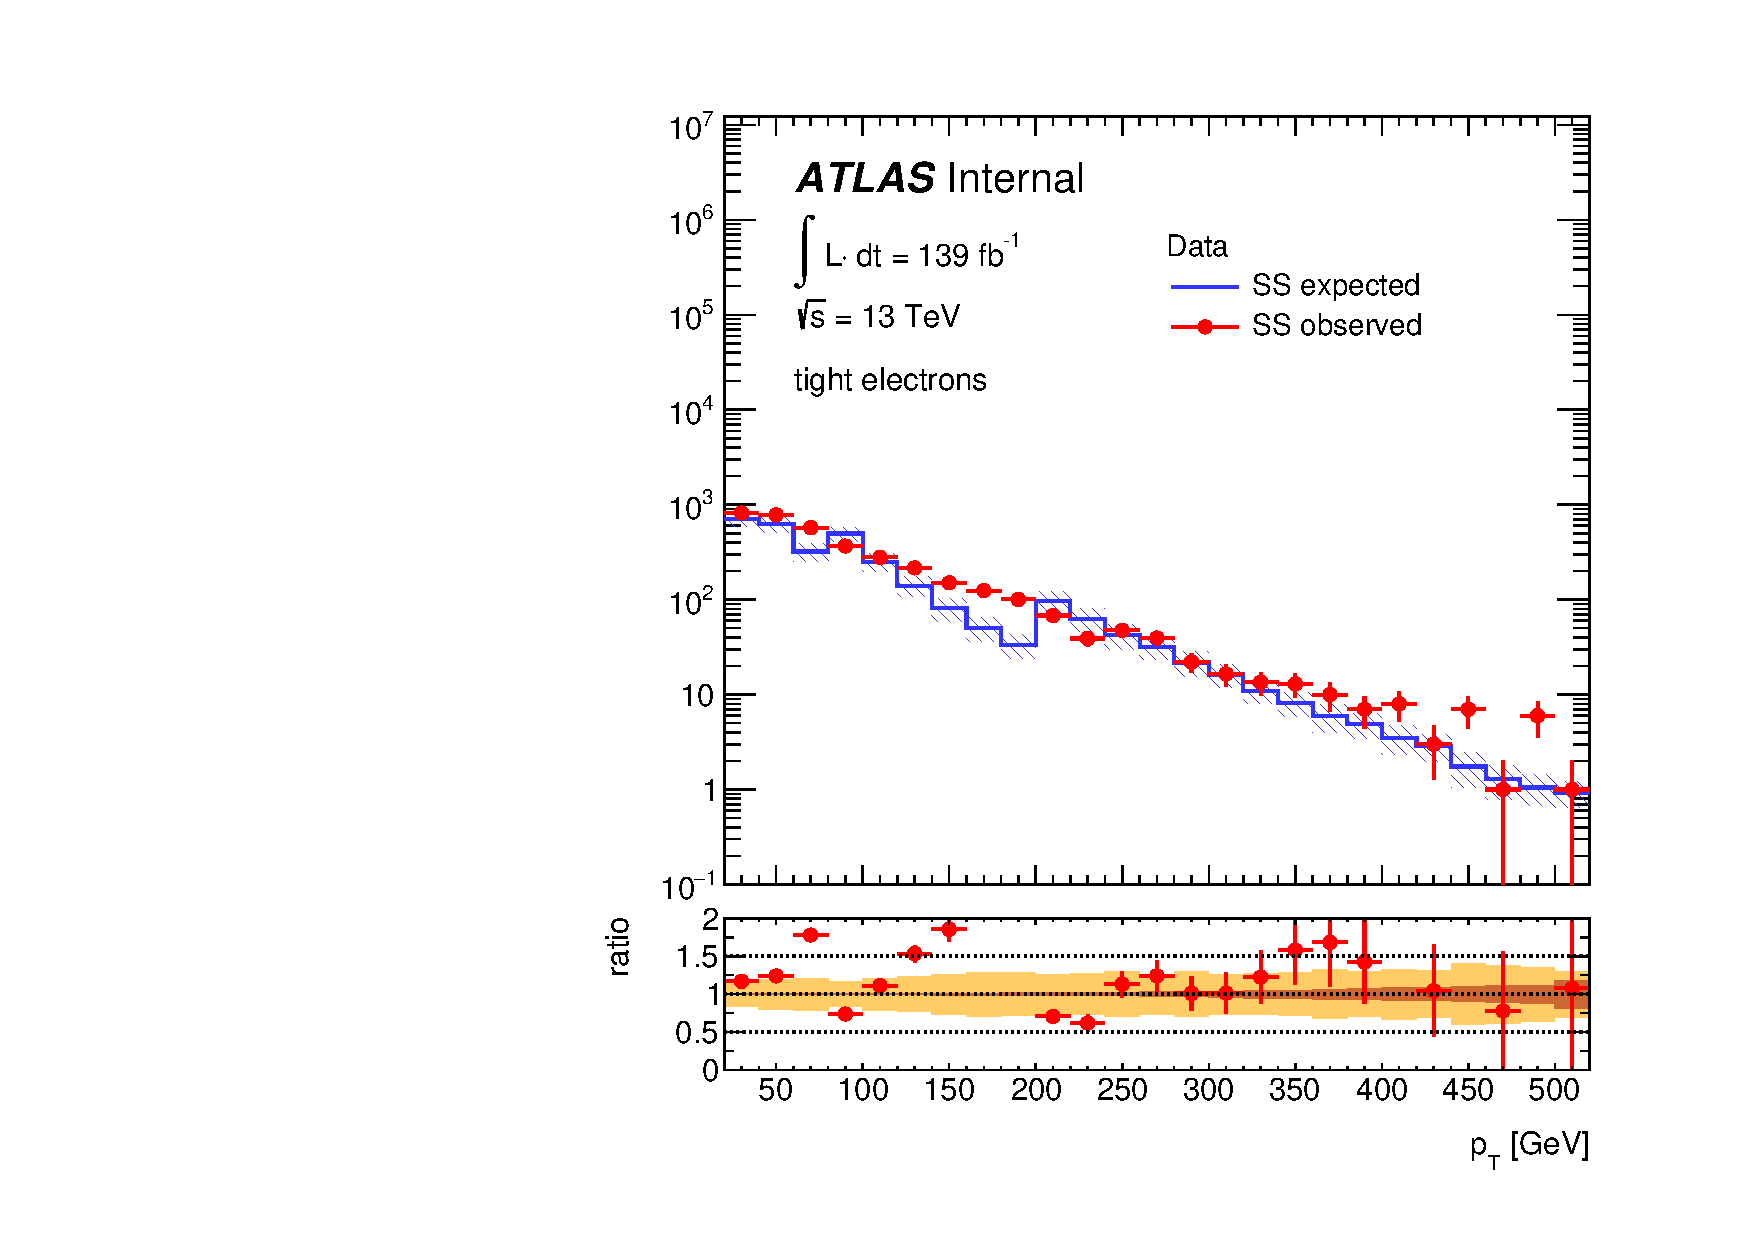
\includegraphics[width=0.45\textwidth]{figures/qmisid/valid_PttightData_binned}
  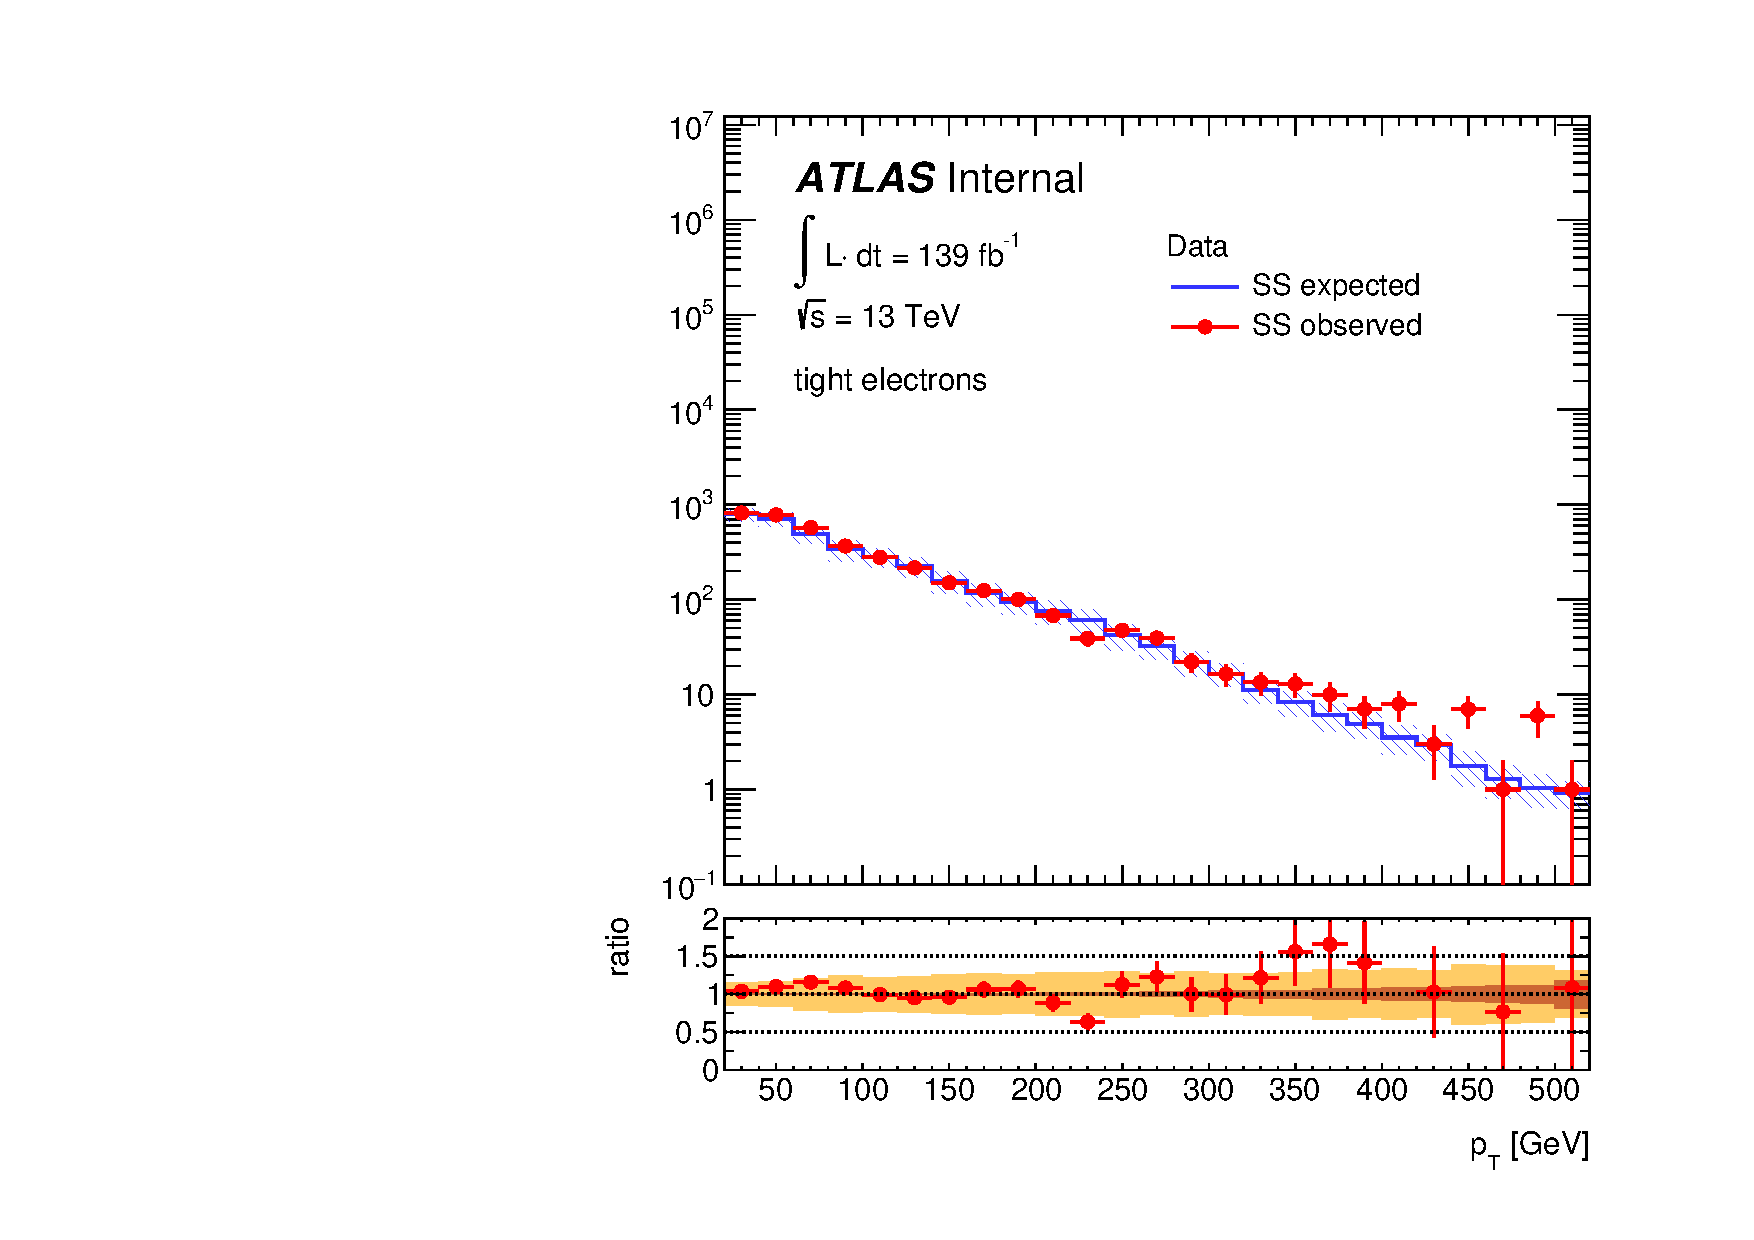
\includegraphics[width=0.45\textwidth]{figures/qmisid/valid_PttightData}\\
  \caption{Comparison between the expected and observed $\pT$ distribution of same-sign electrons.
  The dashed bands represent the total (statistical + systematic) uncertainty of the estimation. The comparison is shown for
  data events. The rates used to compute the predicted distribution are
  binned in $\pT$ (left) or continuous in $\pT$ (right).\label{fig:DatapTJumps}}
\end{figure}


\begin{figure}[tb!]
  \centering
  {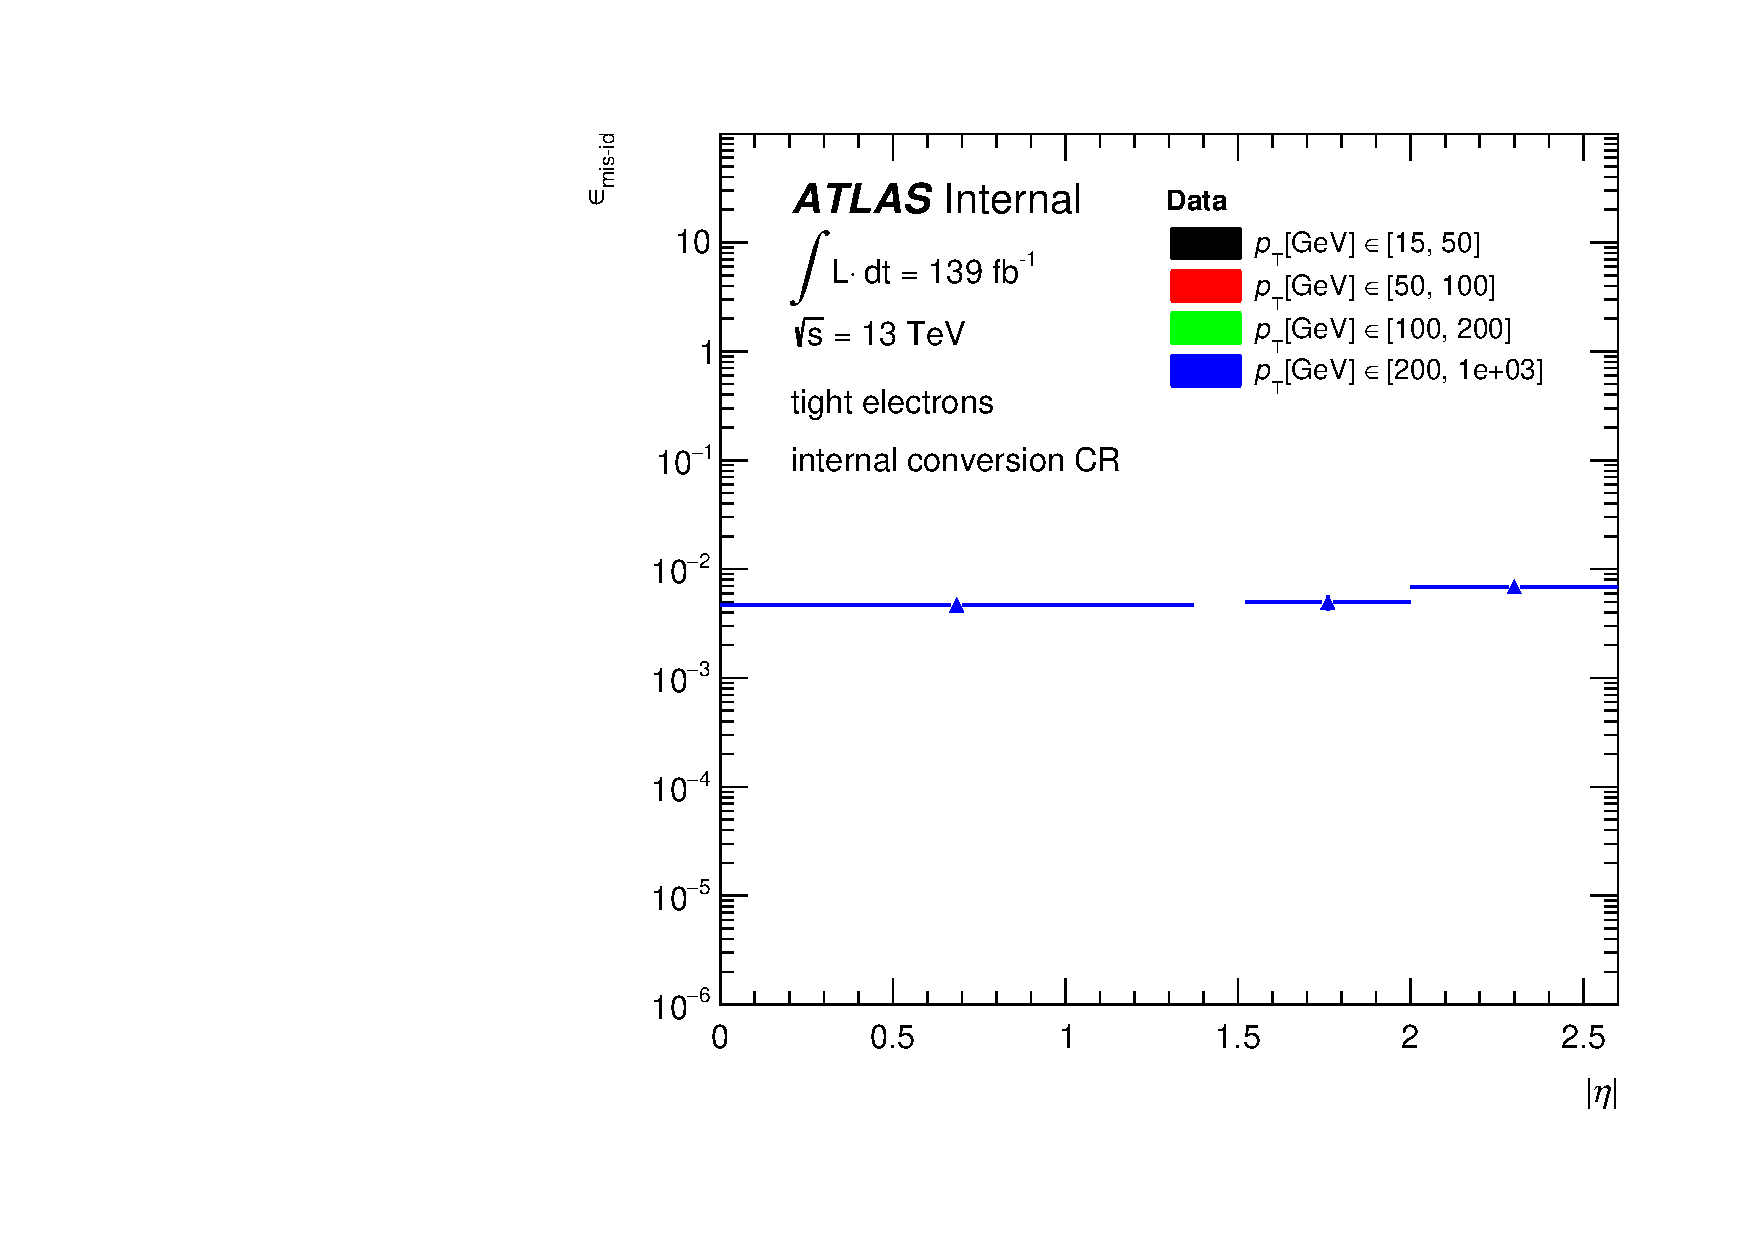
\includegraphics[width=0.37\textwidth]{figures/qmisid/crateData_tight_m0}}
  {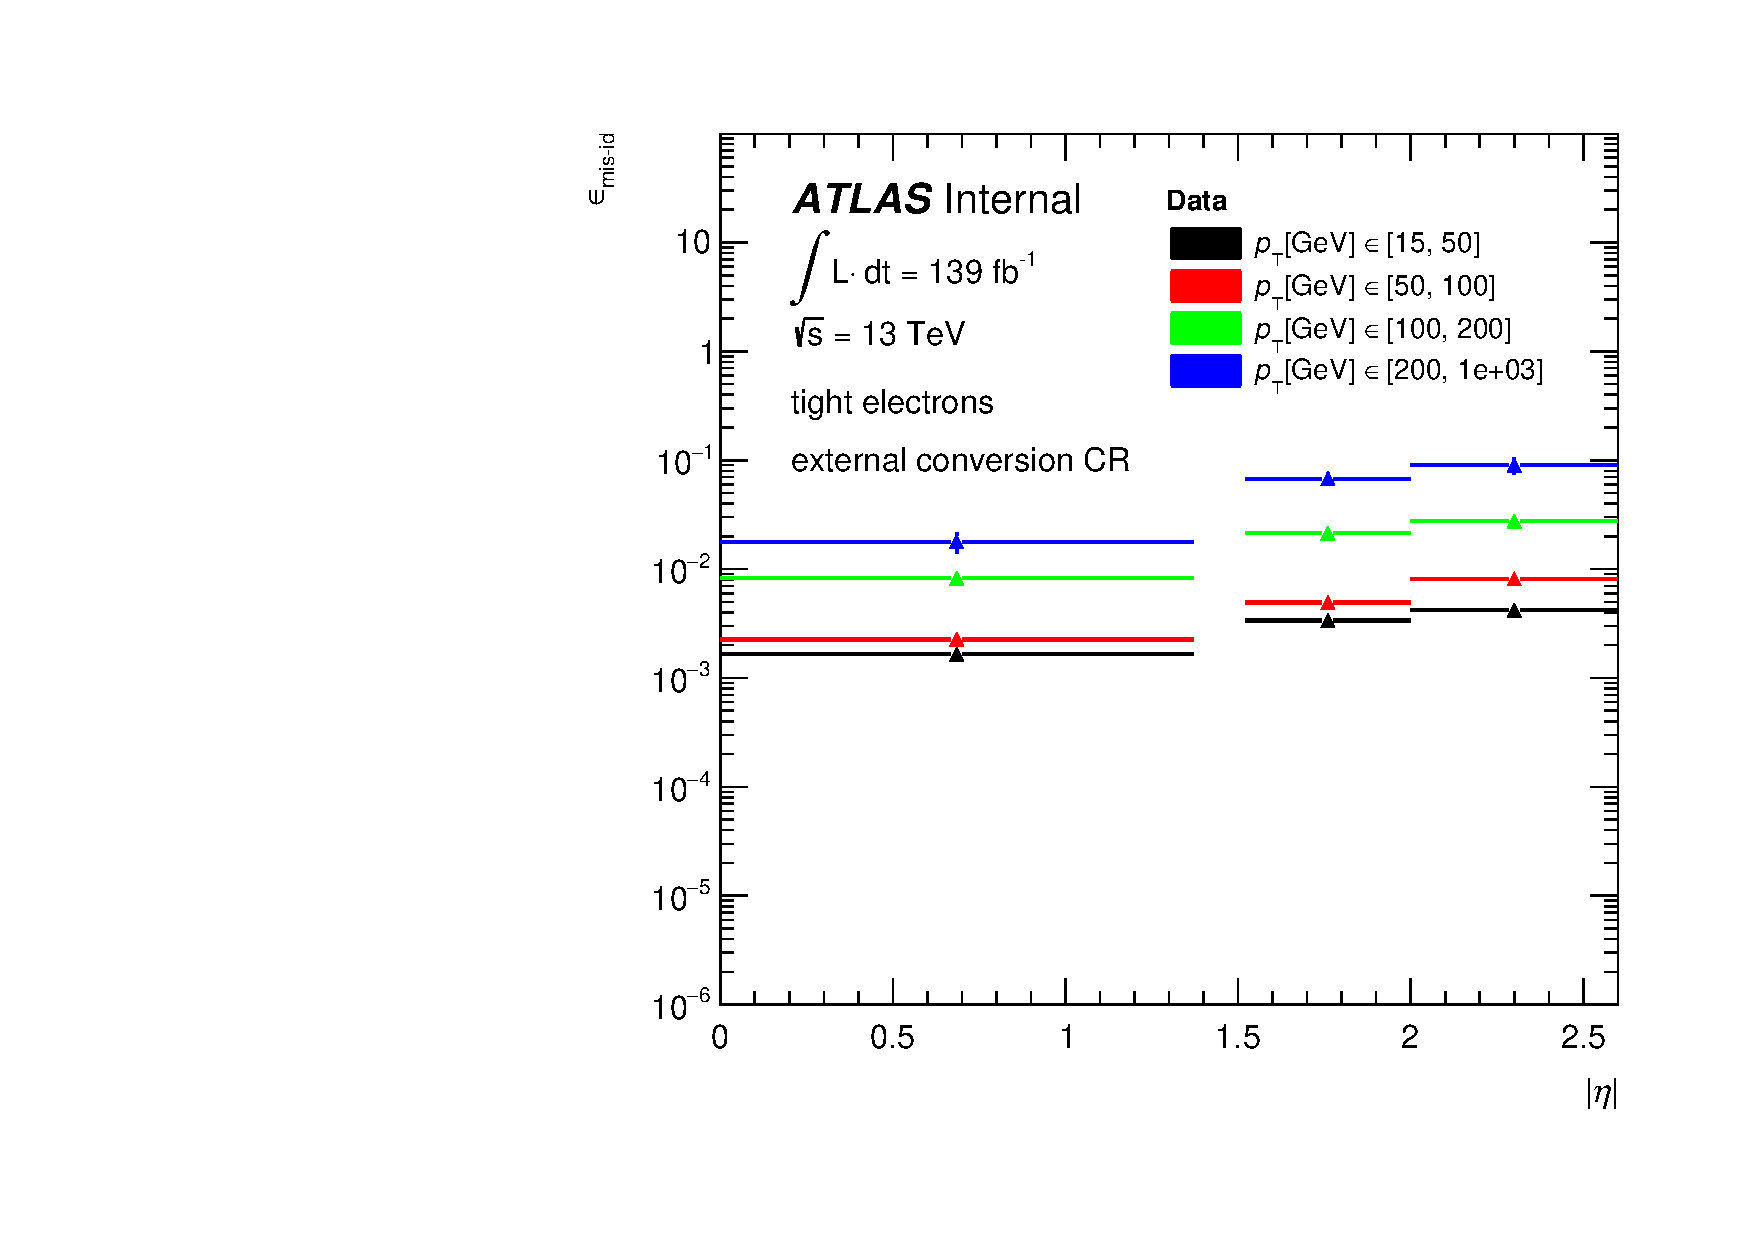
\includegraphics[width=0.37\textwidth]{figures/qmisid/crateData_tight_m1}}\\
  {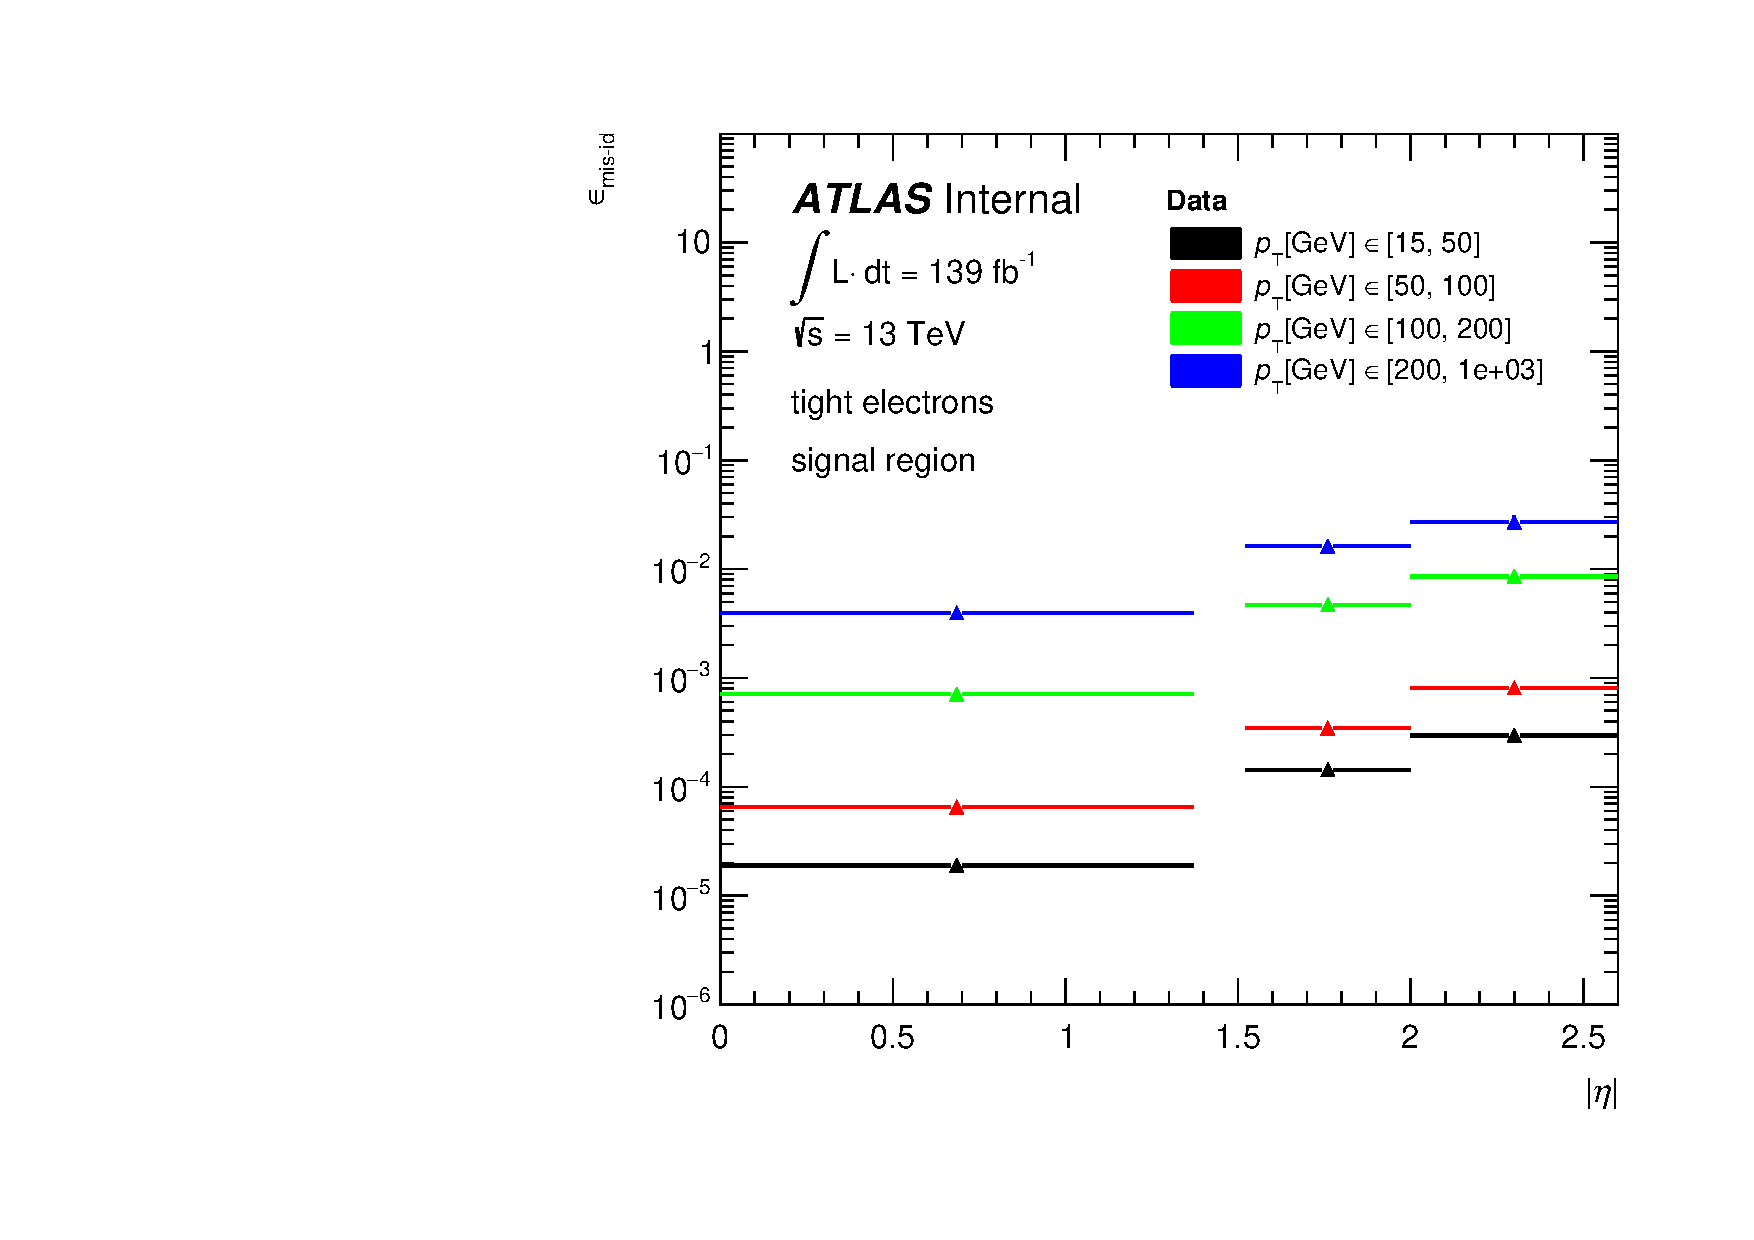
\includegraphics[width=0.37\textwidth]{figures/qmisid/crateData_tight_m2}}
  \caption{QMisID rates derived from the data with the likelihood method for tight electrons. 
           The rates are presented as a function of $|\eta|$ and parameterised in $\pT$ for the 
           photon-conversion CRs and the signal region. Due to lack of statistics, the
           the bins in $\pT$ are merged for the internal-conversion CR.\label{fig:Lik2Ddata}}
\end{figure}

%~~~~~~~~~~~~~~~~~~~~~~~~~~~~~~~~~~~~~~~~~~~~~~~~~~~~~~~~~~~~~~~
\subsubsection{Validation of the likelihood method (truth-closure)}
%~~~~~~~~~~~~~~~~~~~~~~~~~~~~~~~~~~~~~~~~~~~~~~~~~~~~~~~~~~~~~~~

To validate the likelihood method the QMisID rates are derived from simulated $Z$+jets events and compared to the 
rates based on the MC truth information (truth-matching). The comparison is shown in figure\,\ref{fig:LikTruthT} 
as a function of $|\eta|$ and parameterised in $\pT$. To mitigate the large statistical uncertainties introduced due 
to the size of the MC sample, the $|\eta|$-bins are merged. Furthermore, for the internal conversion region, $\pT$ 
bins are also merged. The results show no significant disagreement between the two approaches. Any difference is 
considered as a systematic uncertainty to the rates (see section\,\ref{Sec:systematic}). Finally, the same comparison 
is presented for the case of anti-tight electrons in order to verity the agreement of the two approaches with 
higher statistics.  

\begin{figure}[tb!]
  \centering
  {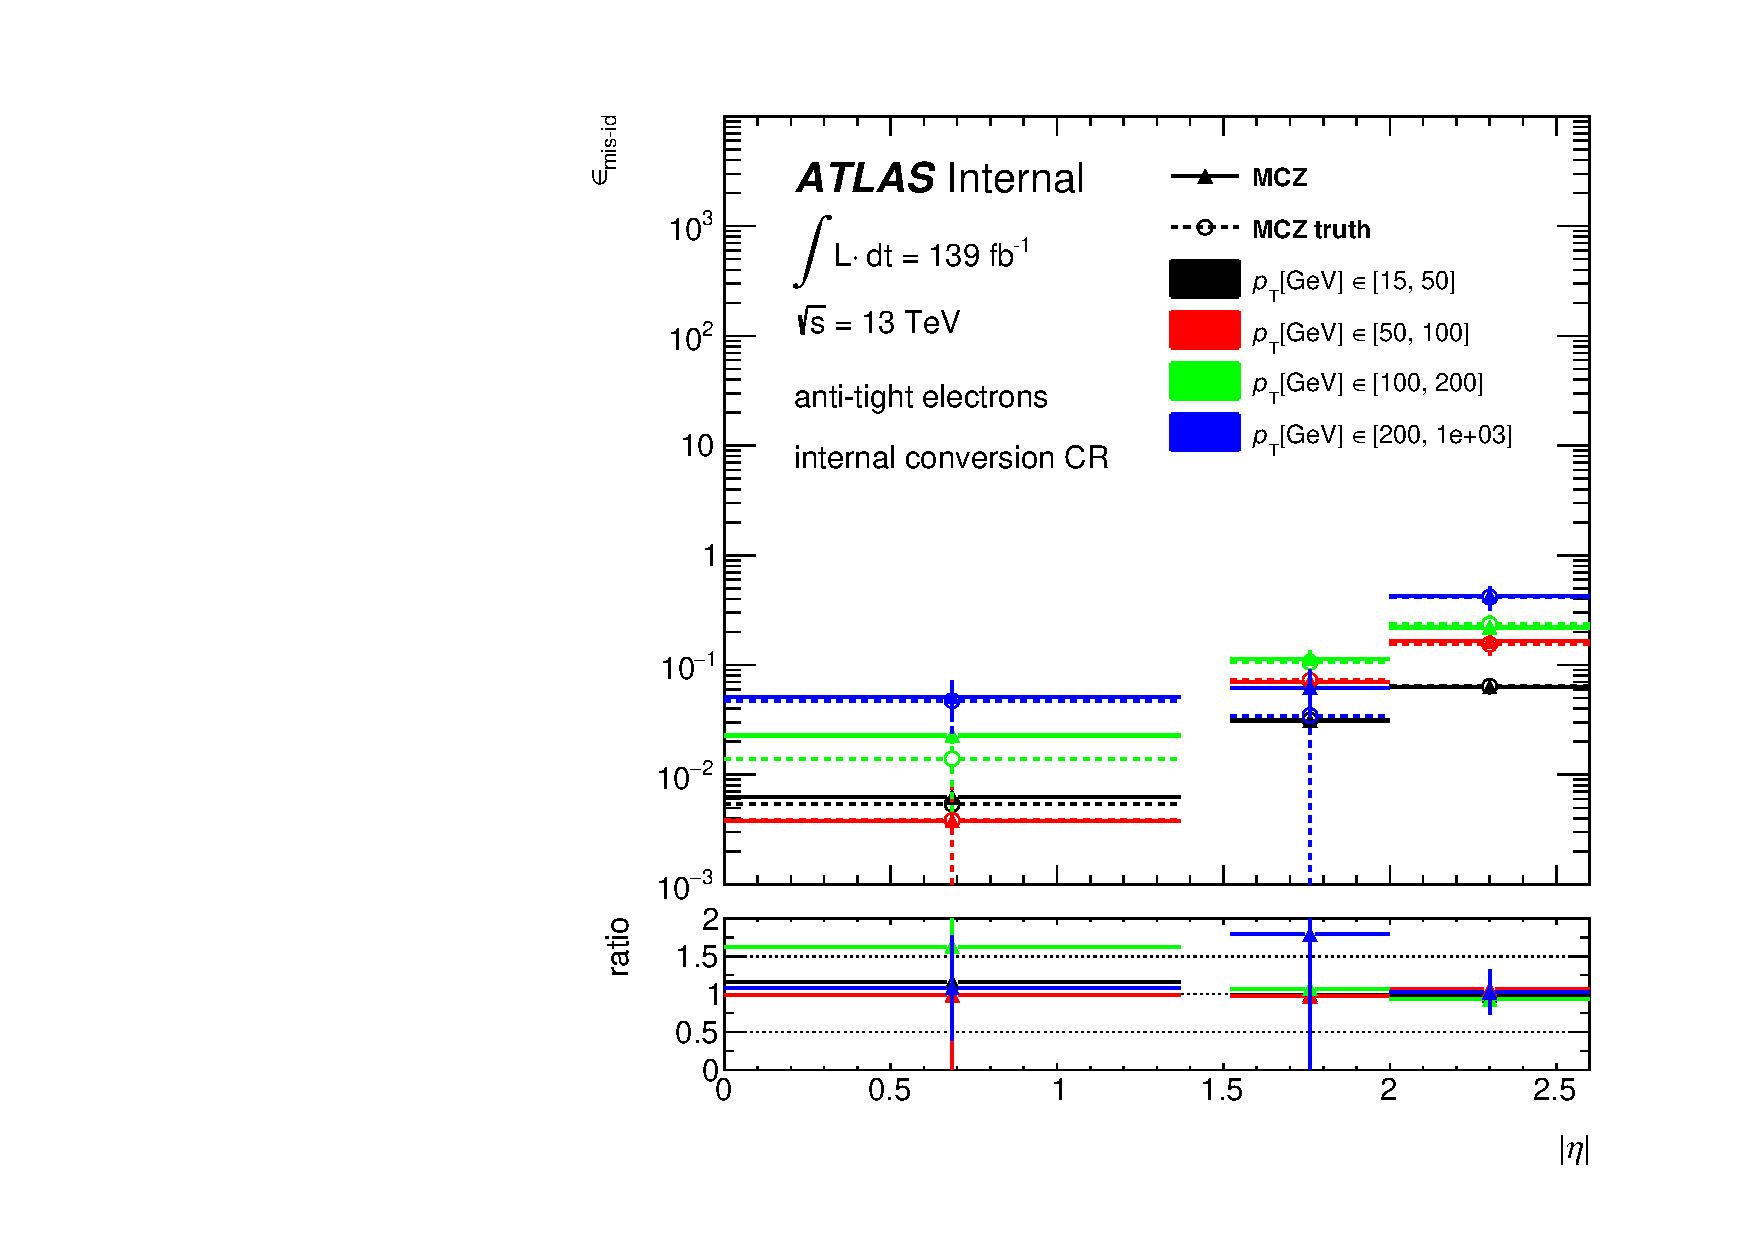
\includegraphics[width=0.45\textwidth]{figures/qmisid/crateMCZ_MCZtruth_atight_m0}}
  {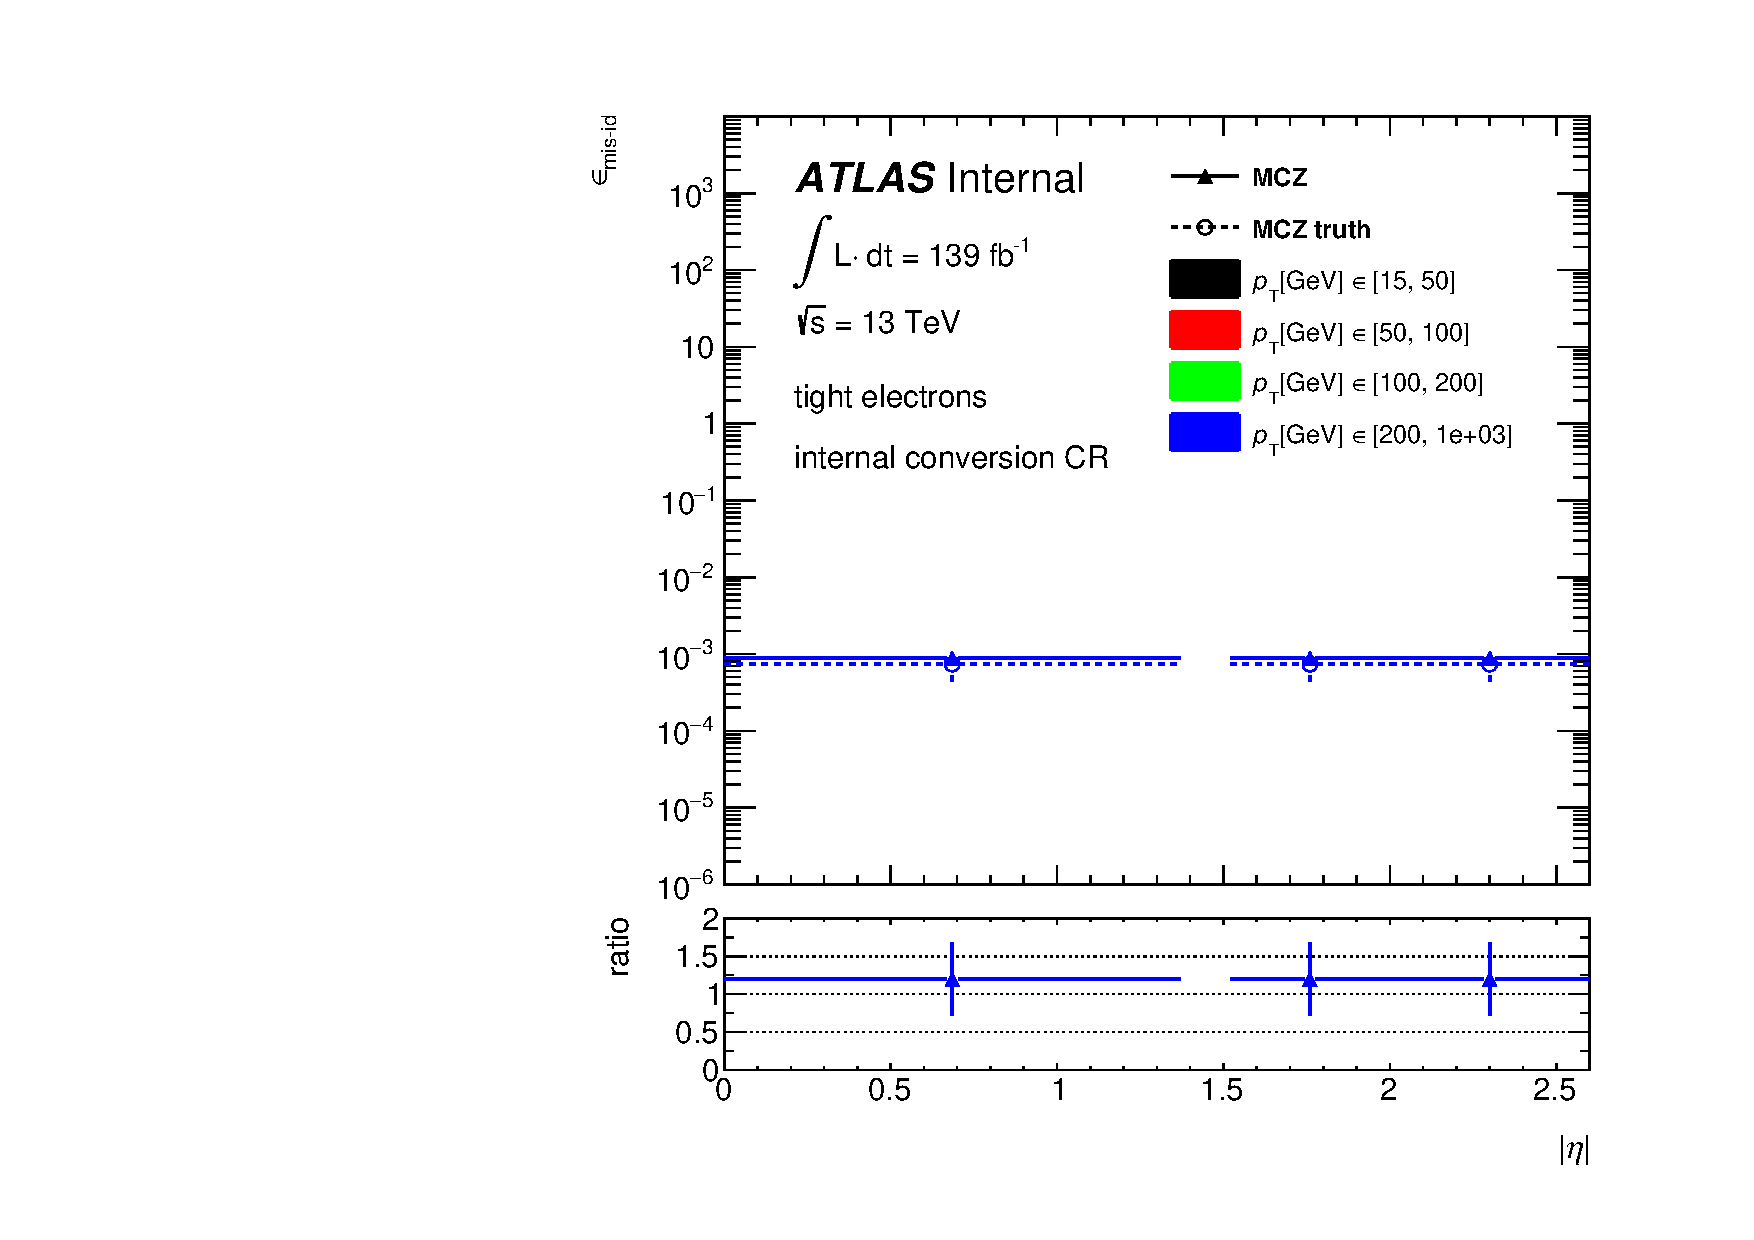
\includegraphics[width=0.45\textwidth]{figures/qmisid/crateMCZ_MCZtruth_tight_m0}}\\
  {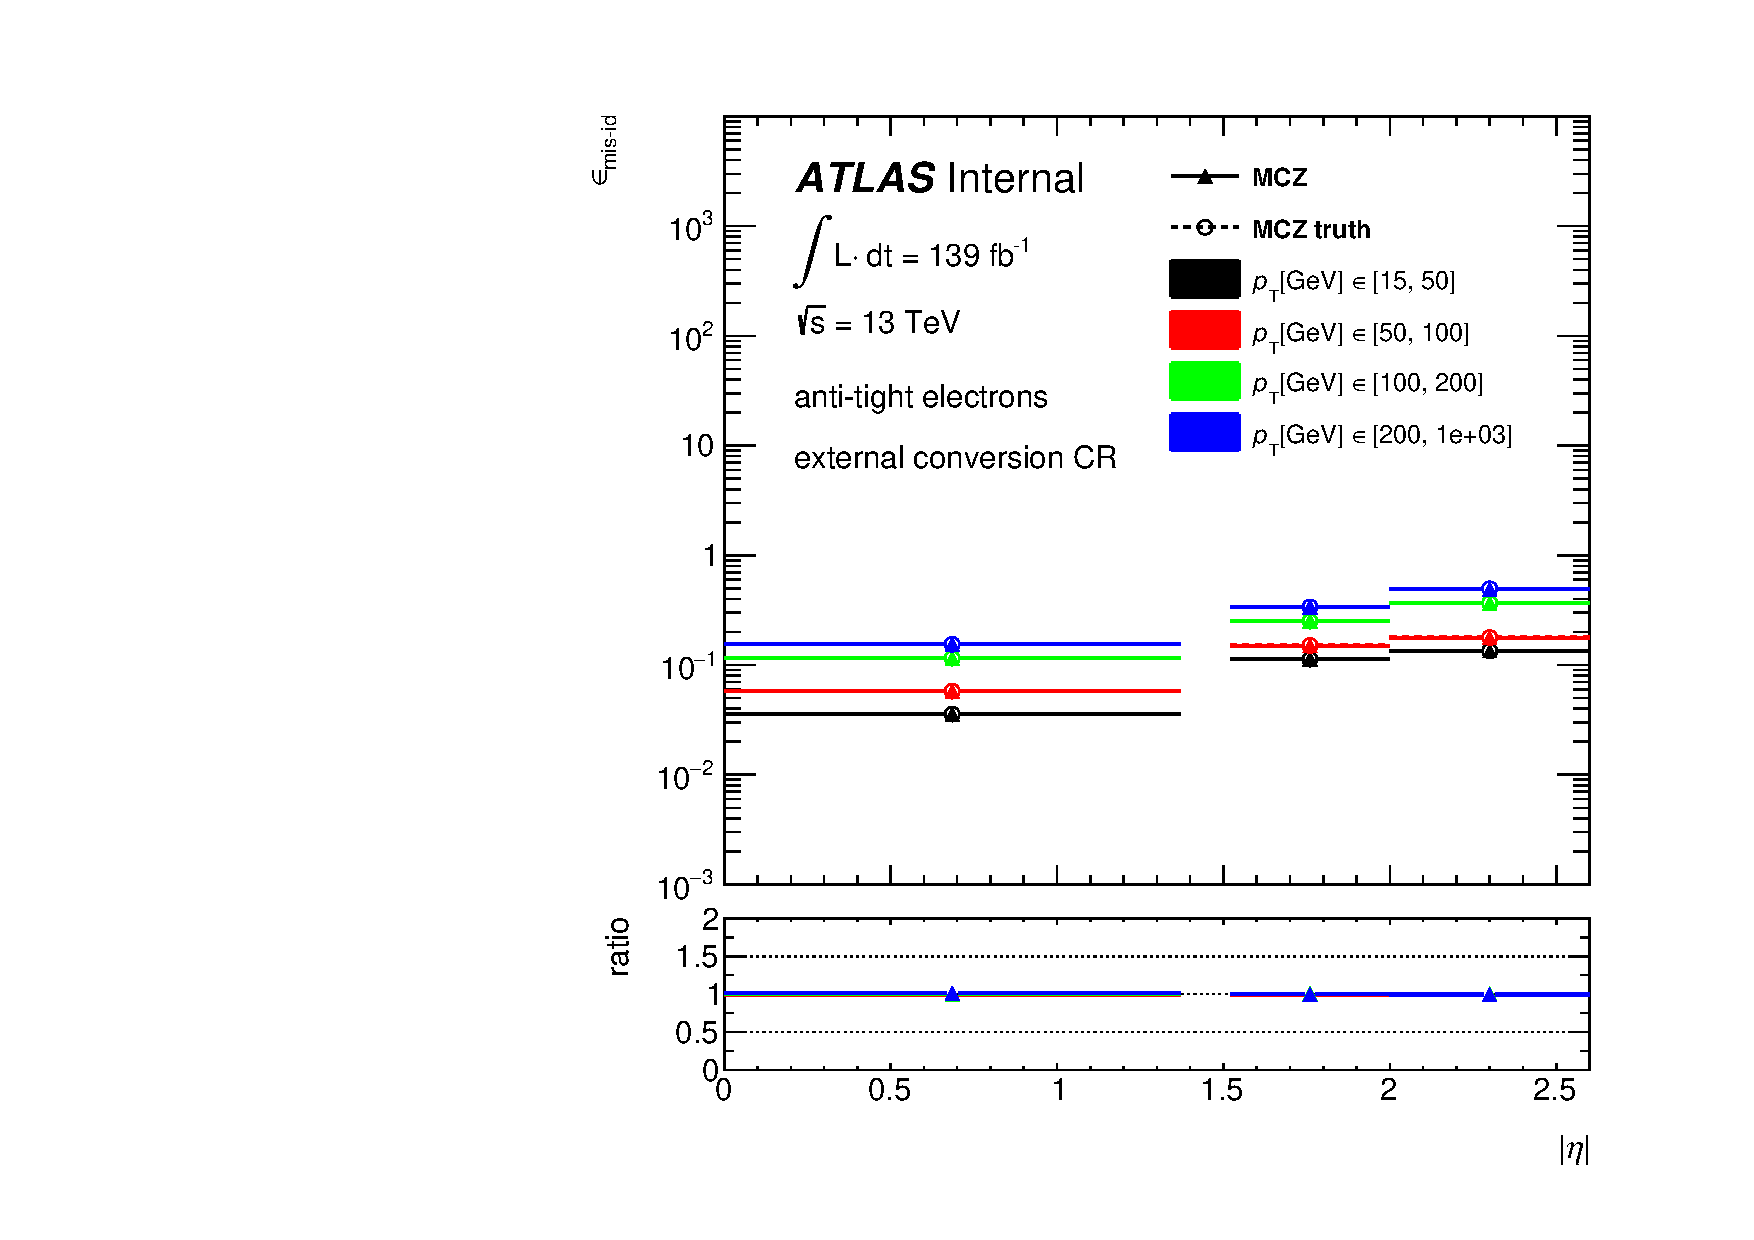
\includegraphics[width=0.45\textwidth]{figures/qmisid/crateMCZ_MCZtruth_atight_m1}}
  {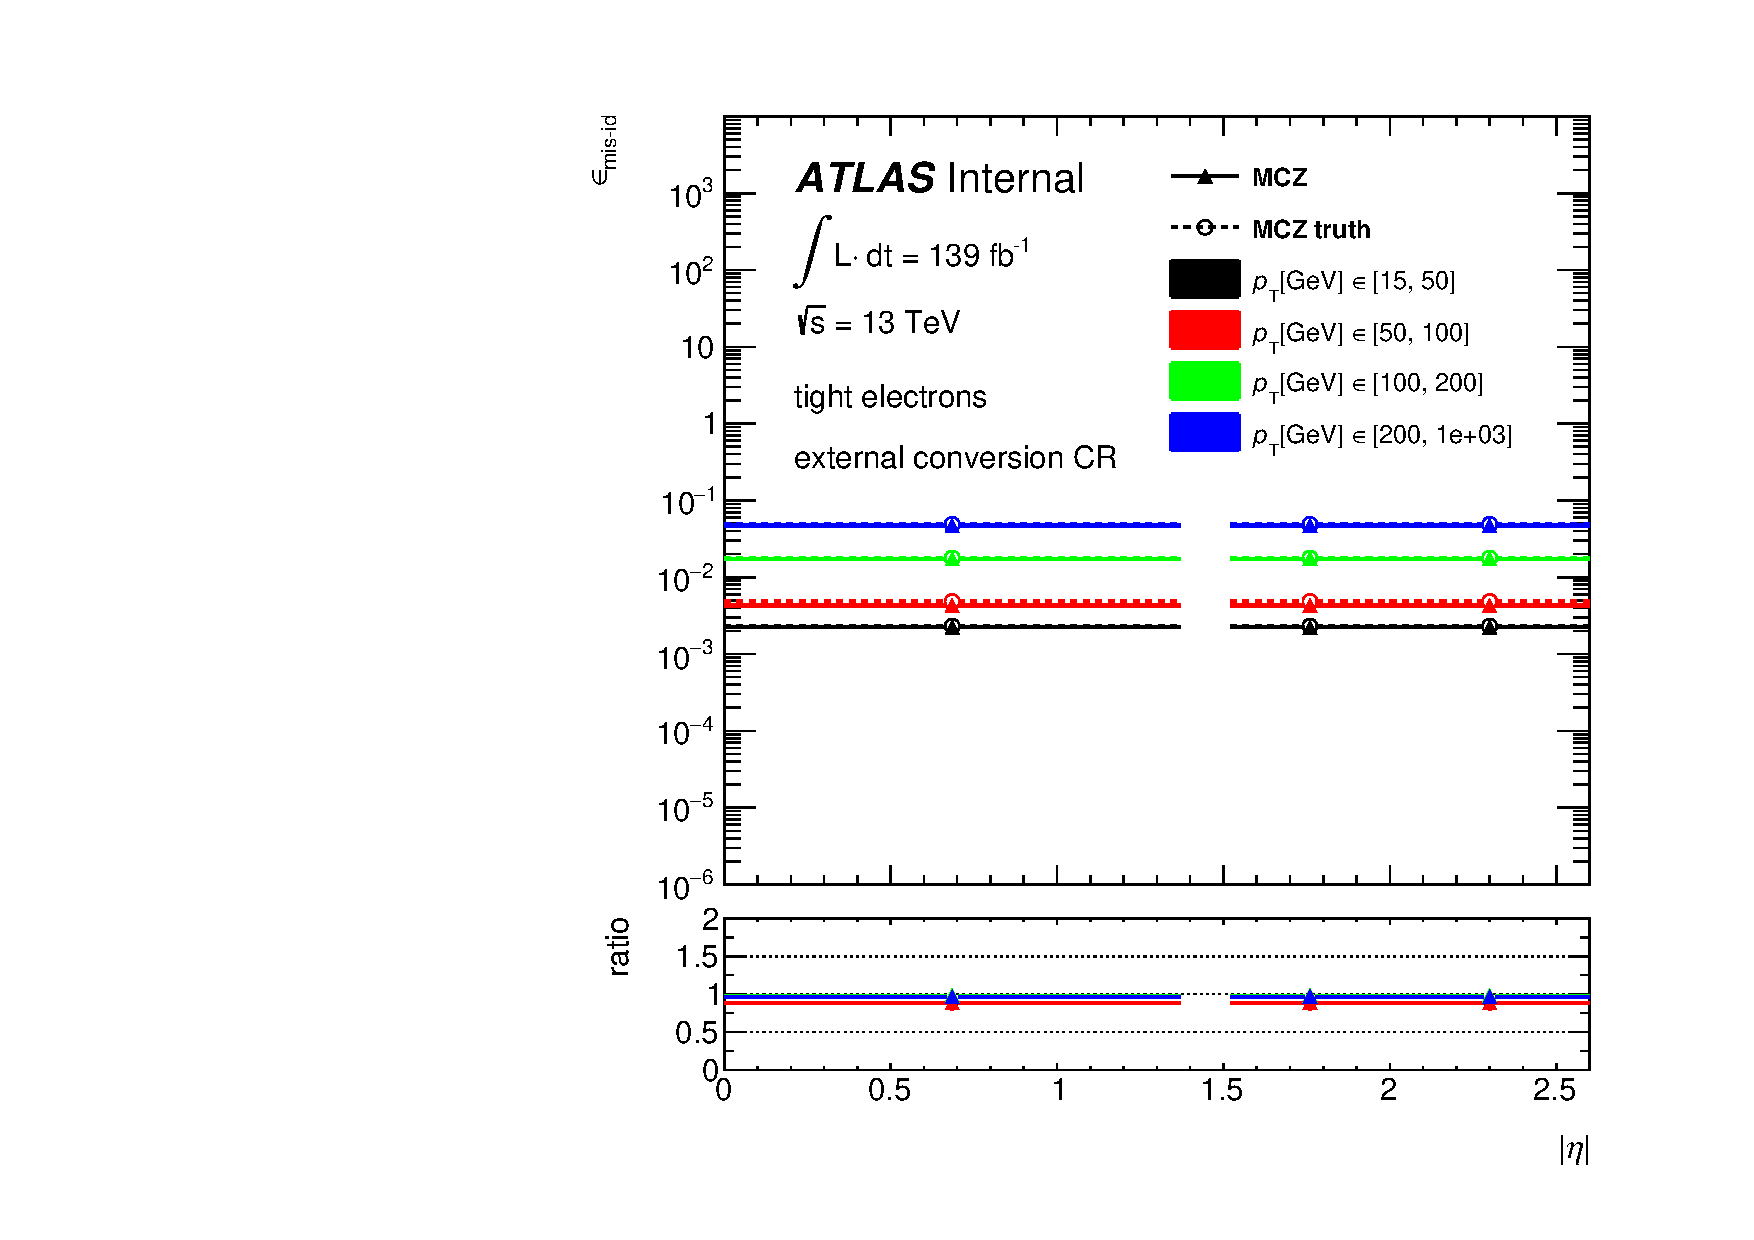
\includegraphics[width=0.45\textwidth]{figures/qmisid/crateMCZ_MCZtruth_tight_m1}}\\
  {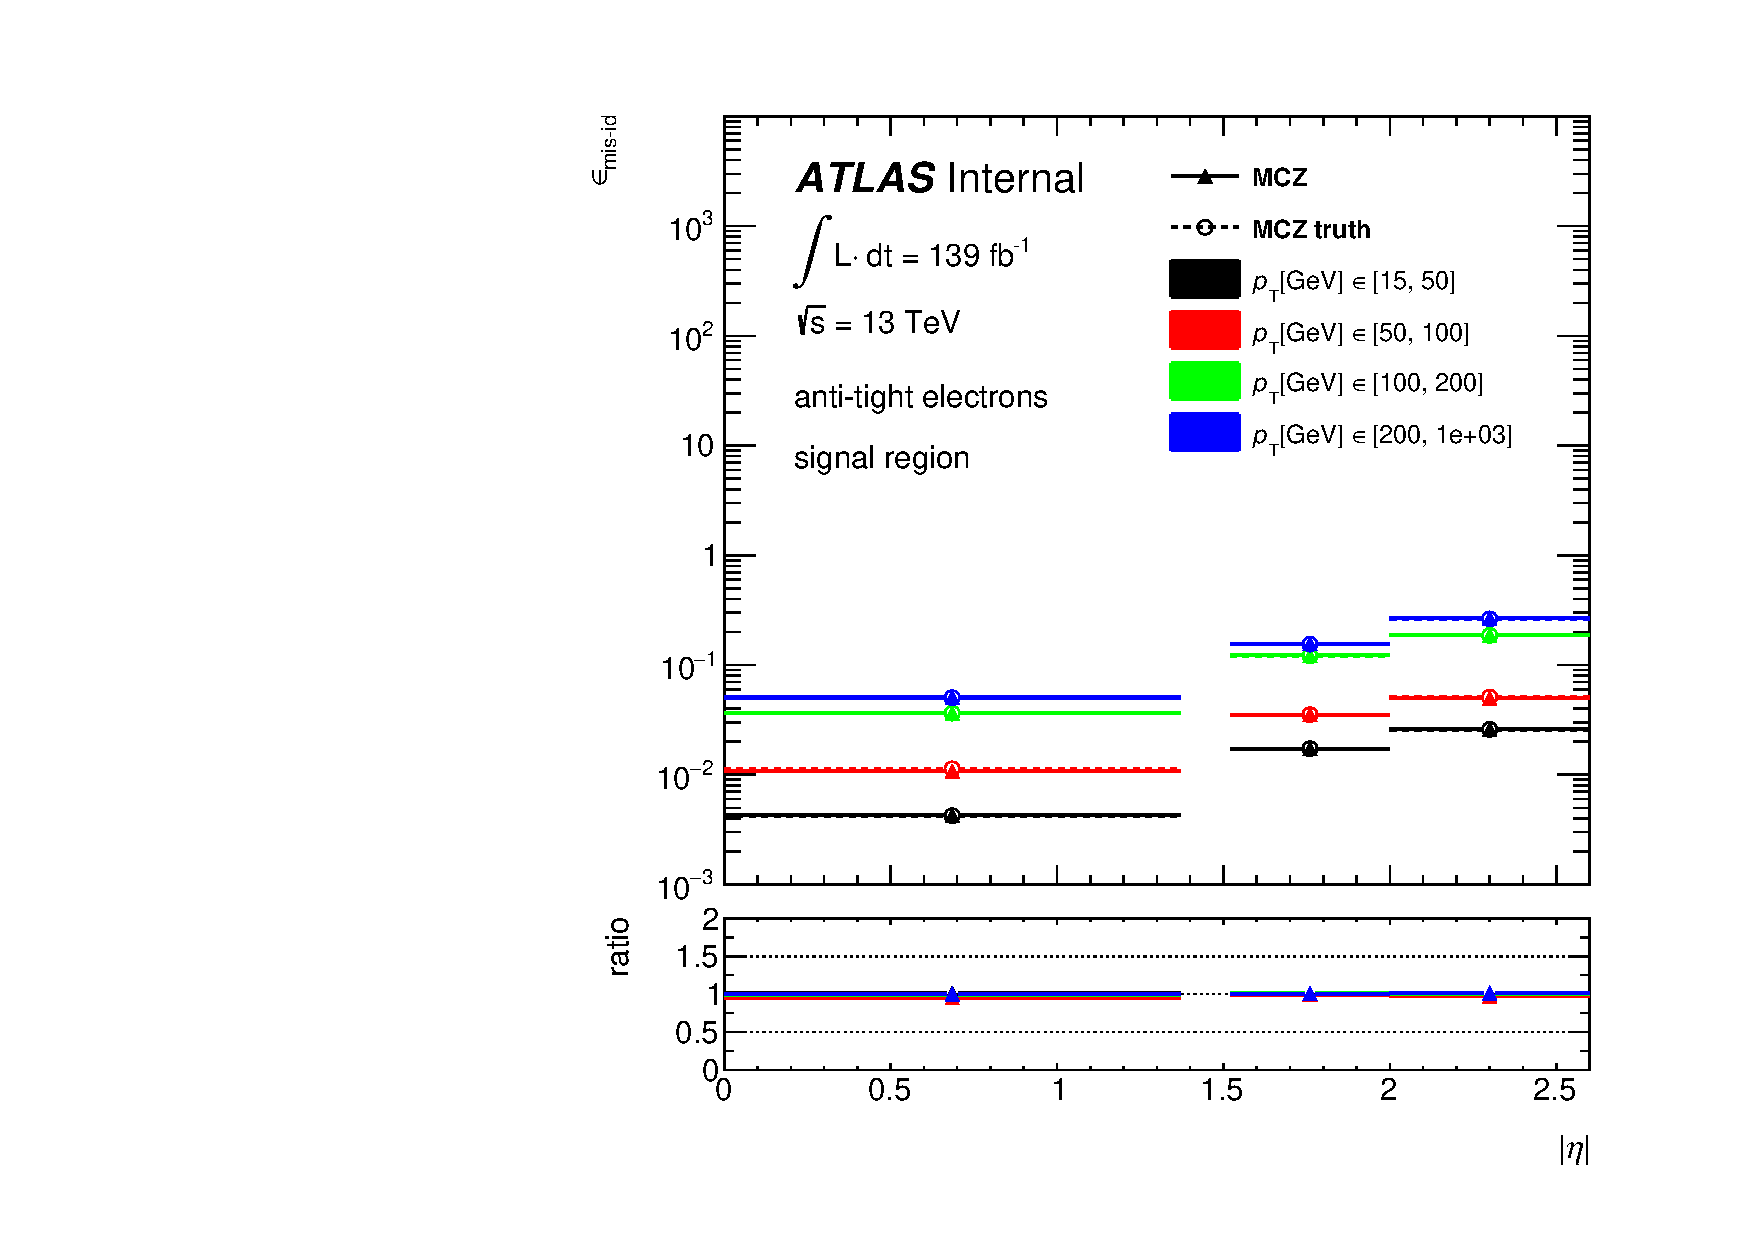
\includegraphics[width=0.45\textwidth]{figures/qmisid/crateMCZ_MCZtruth_atight_m2}}
  {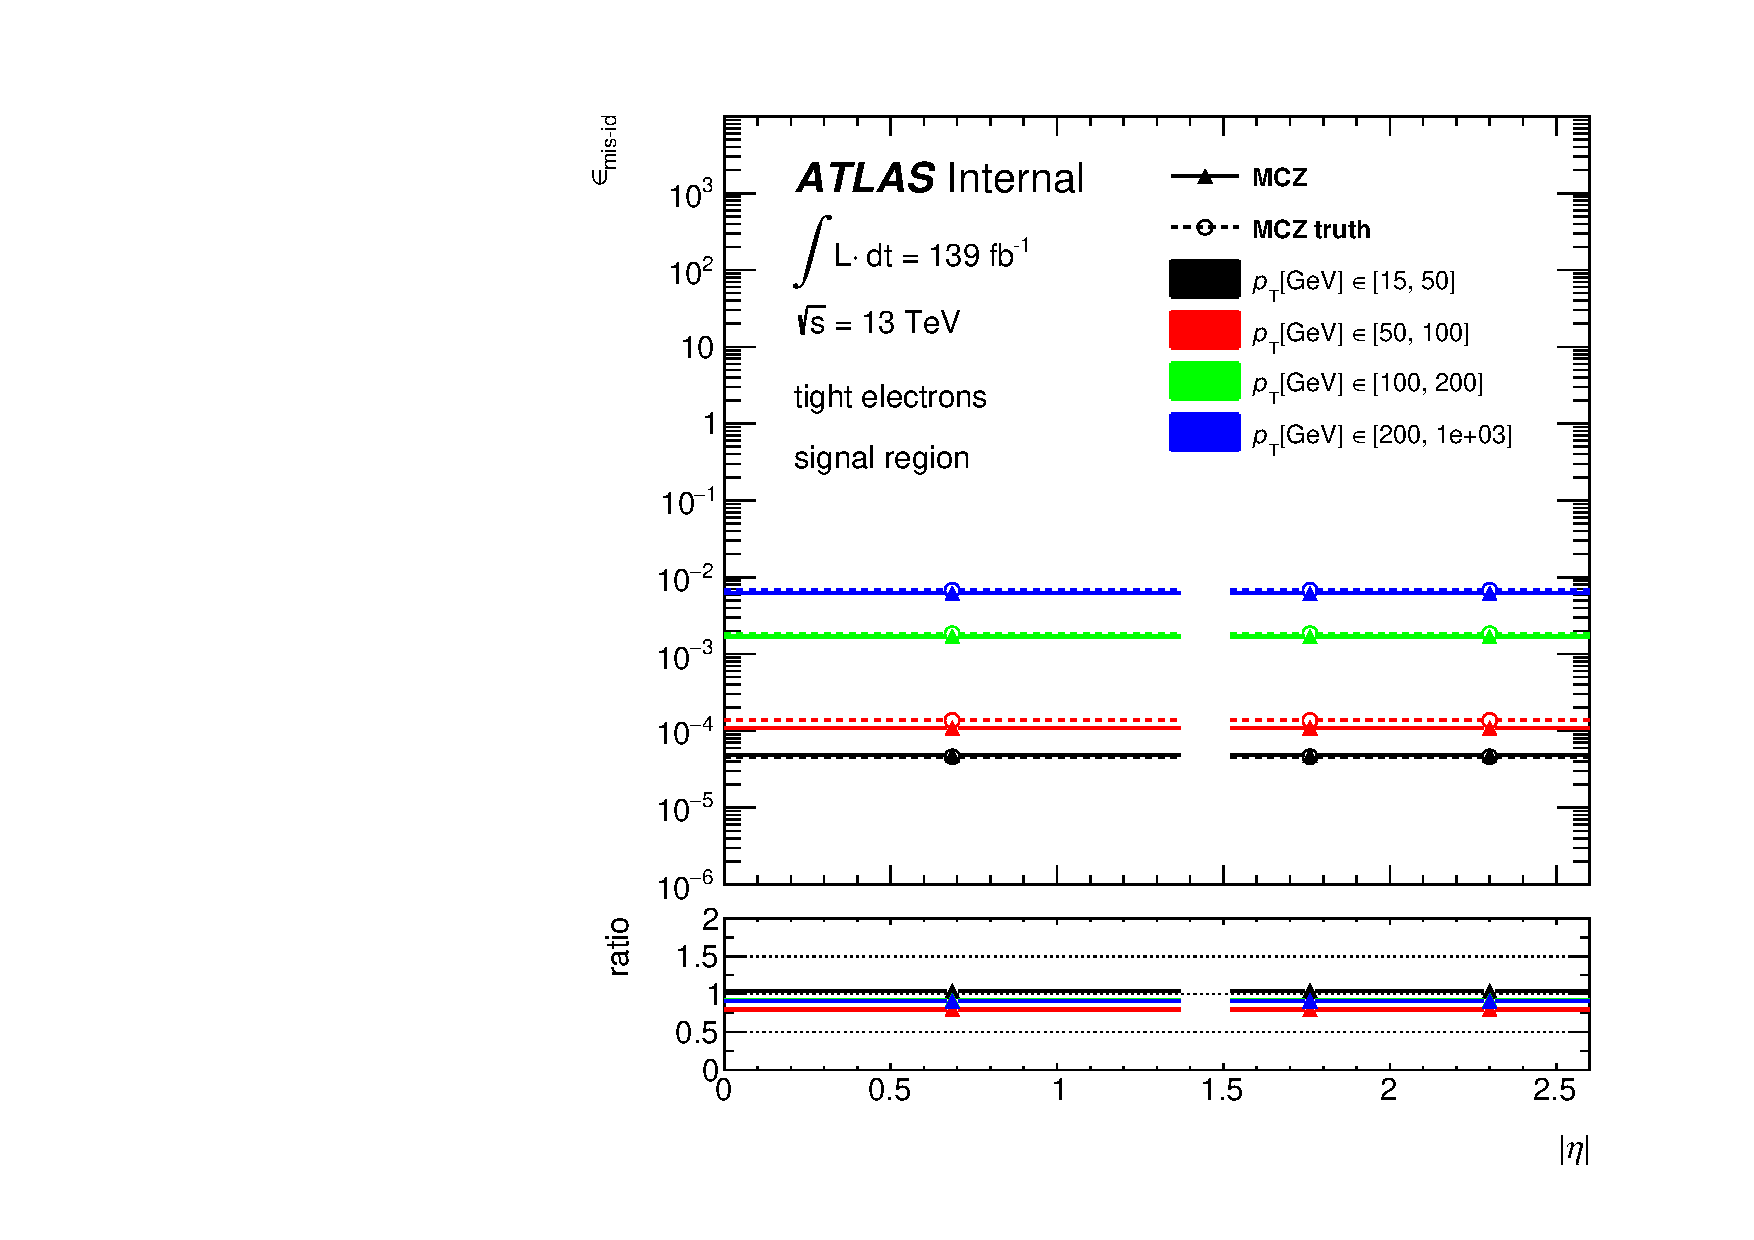
\includegraphics[width=0.45\textwidth]{figures/qmisid/crateMCZ_MCZtruth_tight_m2}}
  \caption{QMisID rates derived from $Z\rightarrow ee$ simulated events with the likelihood method, compared to truth-based
           rates for anti-tight (left) and tight (right) electrons. The rates are presented as a function of $|\eta|$,
           parameterised in $\pT$ for the photon-conversion CRs and the signal region. Due to lack of statistics, in 
           the case of tight electrons, the bins in $|\eta|$ are merged. For the internal-conversion CR, the bins in 
           $\pT$ are also merged.\label{fig:LikTruthT}}
\end{figure}

\clearpage

%~~~~~~~~~~~~~~~~~~~~~~~~~~~~~~~~~~~
\subsubsection{Systematic uncertainties}
\label{Sec:systematic}
%~~~~~~~~~~~~~~~~~~~~~~~~~~~~~~~~~~~

Four sources of systematic uncertainties are assigned to the QMisiD rates:

\begin{itemize}
\item the error estimates from the likelihood maximisation (figure\,\ref{fig:QMisID:systa}) which depend on the 
      statistical size of the control region of the data in which the rates are estimated;
\item the difference between the rates measured with the likelihood method and those obtained by truth-matching 
      with simulated $Z\rightarrow ee$ events (figure\,\ref{fig:QMisID:systa});
\item the variation of the rates with the $m_Z$ window
  (figure\,\ref{fig:QMisID:systb});
\item low $m_{ee}$ mismodelings observed on simulated $t\bar{t}$ samples and
  that can be relevant to some control regions.
\end{itemize}

The total uncertainty is defined as the quadratic sum of the above contributions (figure\,\ref{fig:QMisID:systb}).

\begin{figure}[p!]
  \begin{center}
  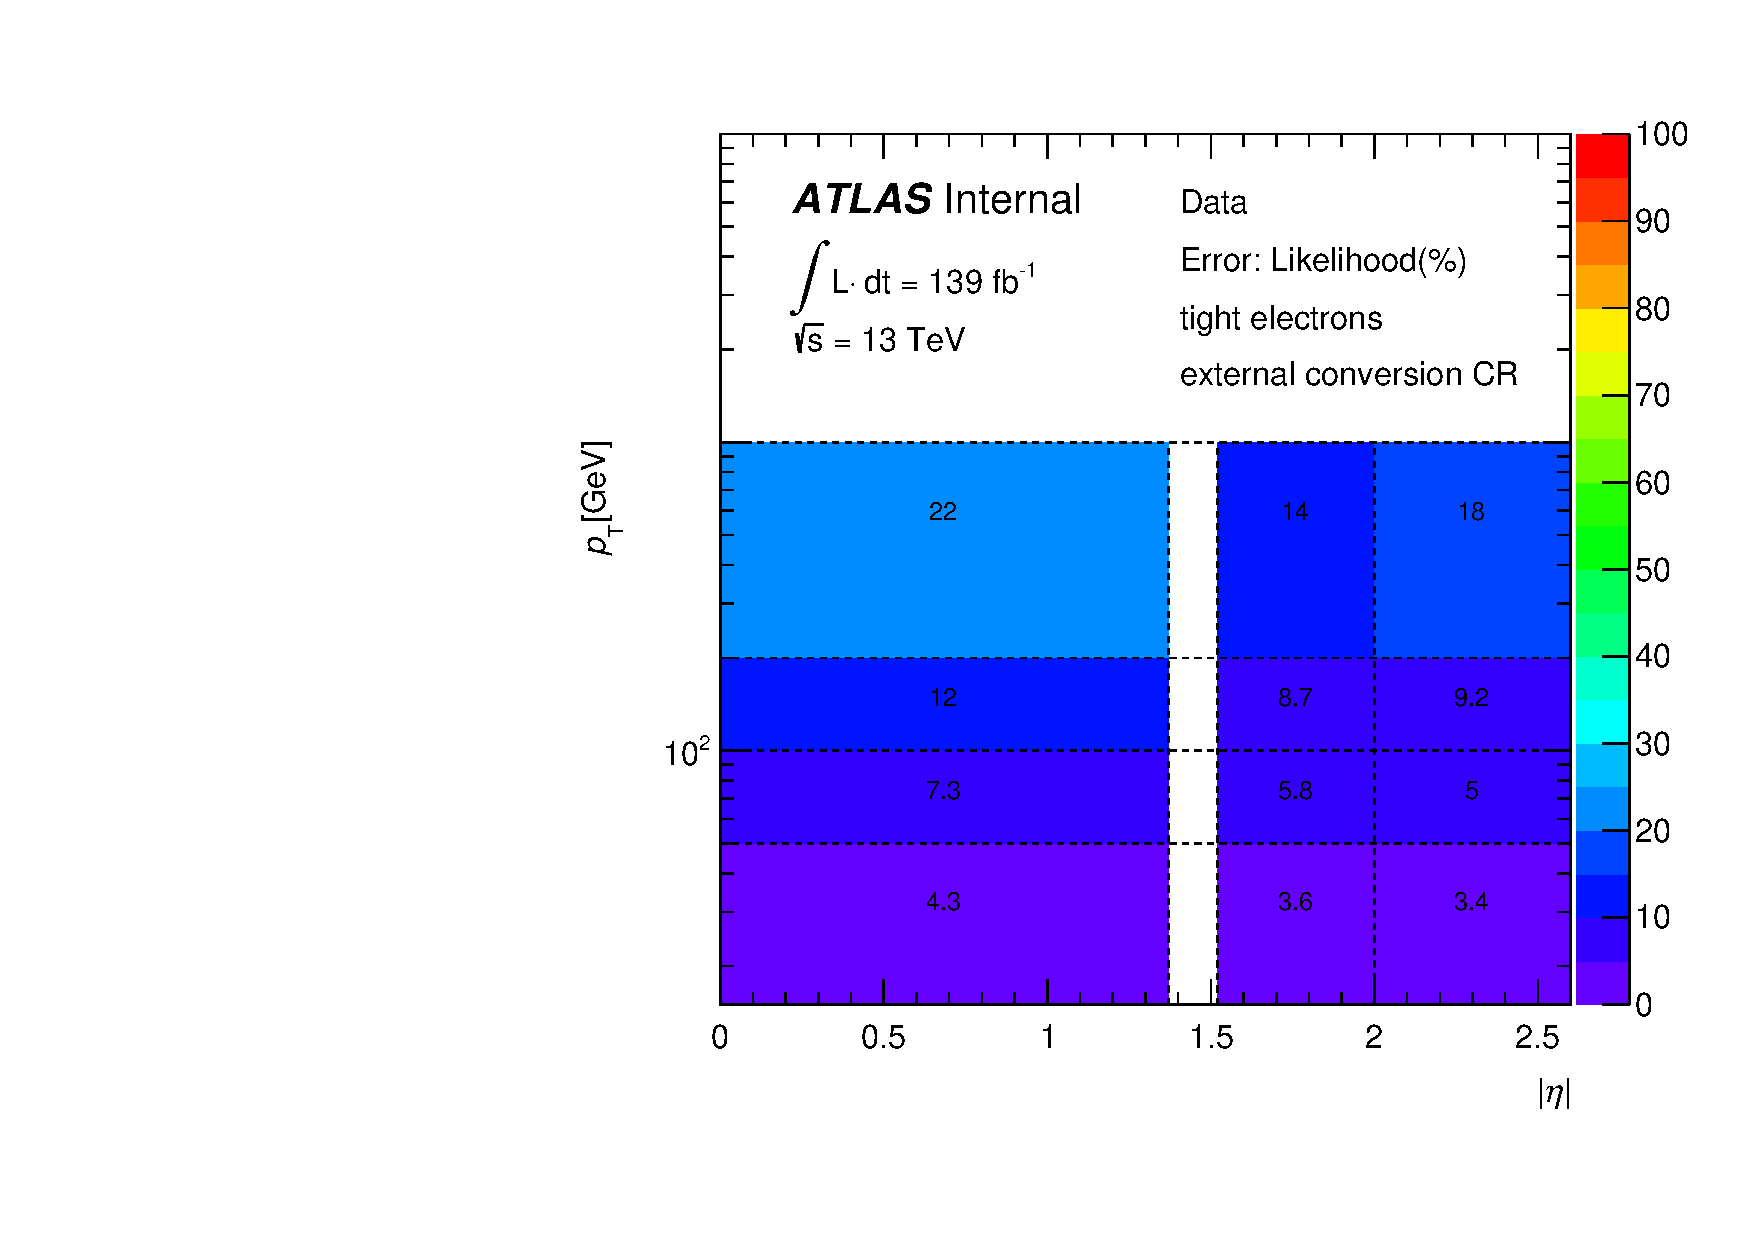
\includegraphics[width=0.45\textwidth]{figures/qmisid/syst_Data_Likelihood_tight_extcr}
  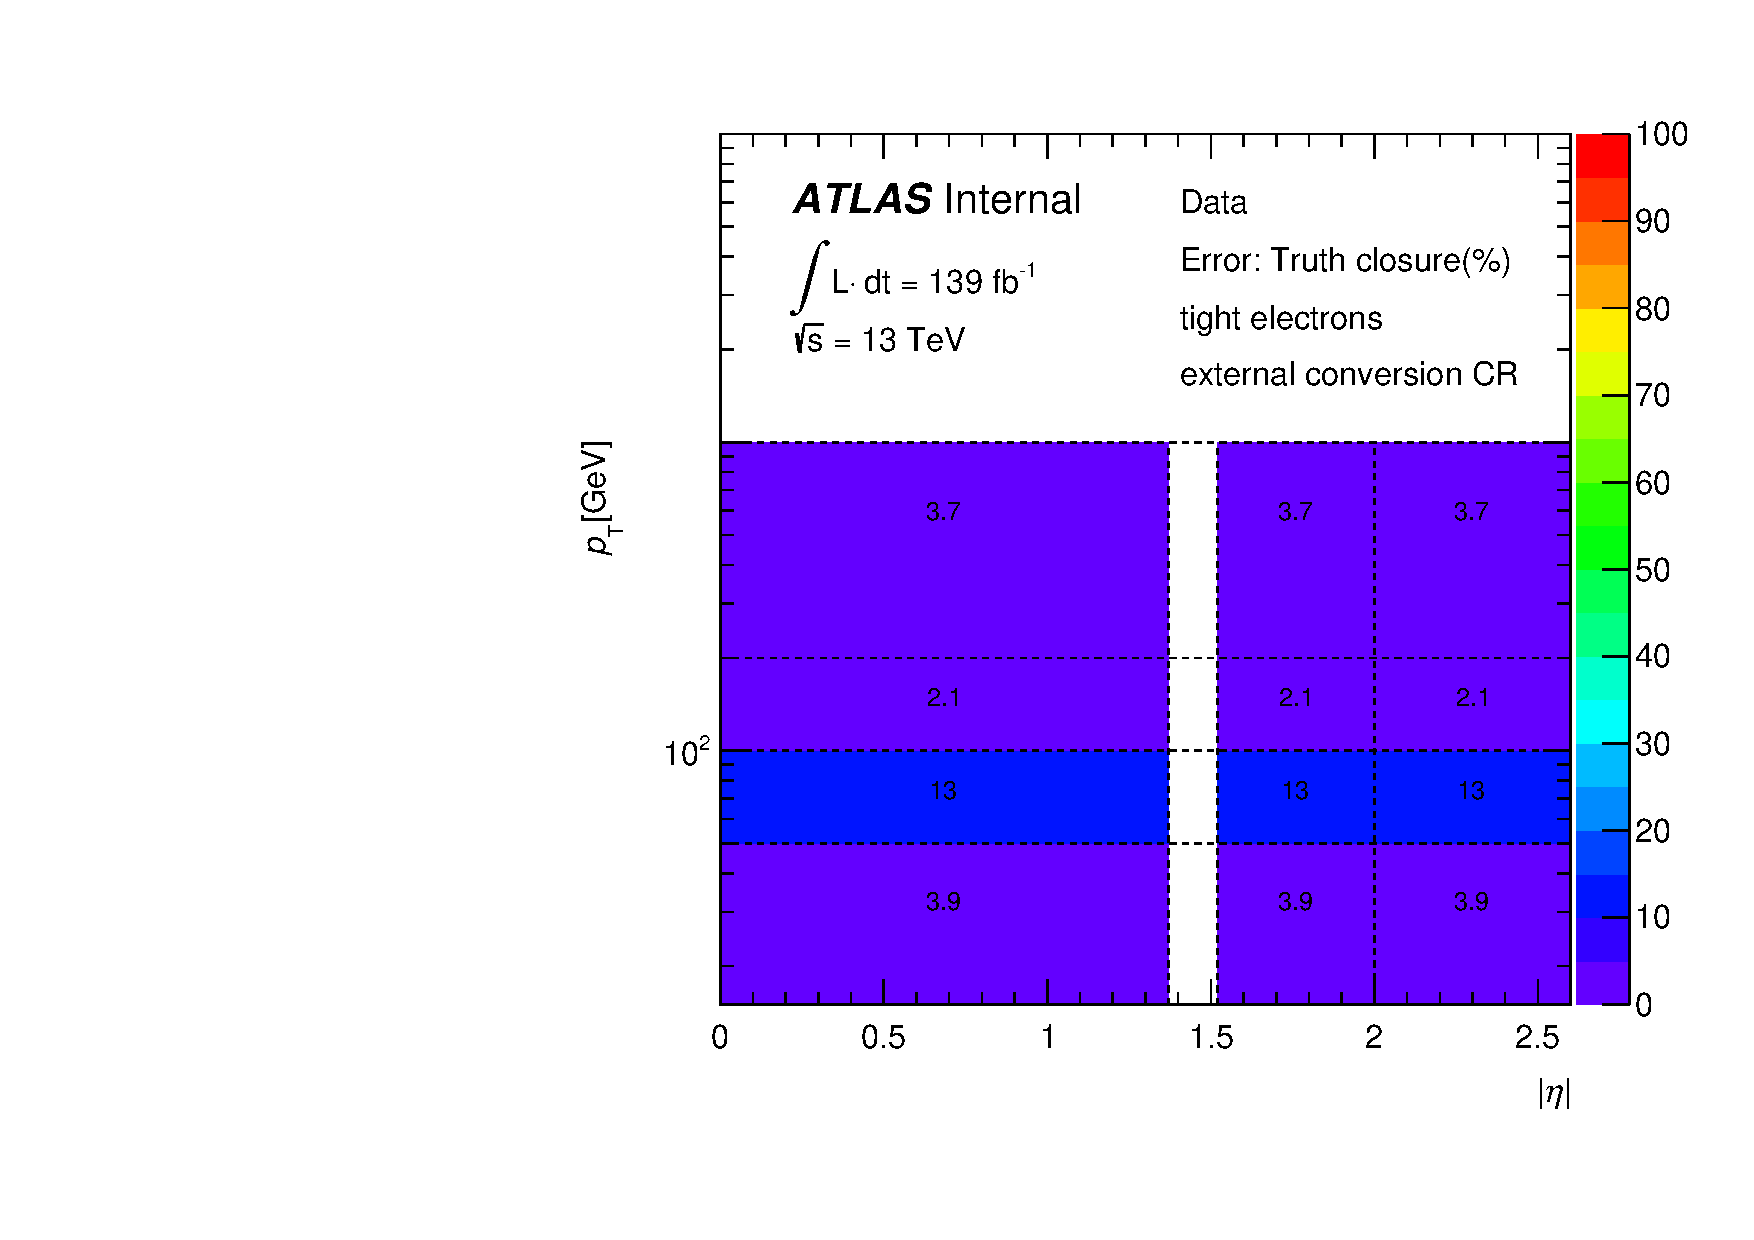
\includegraphics[width=0.45\textwidth]{figures/qmisid/syst_Data_Truthclosure_tight_extcr}\\
  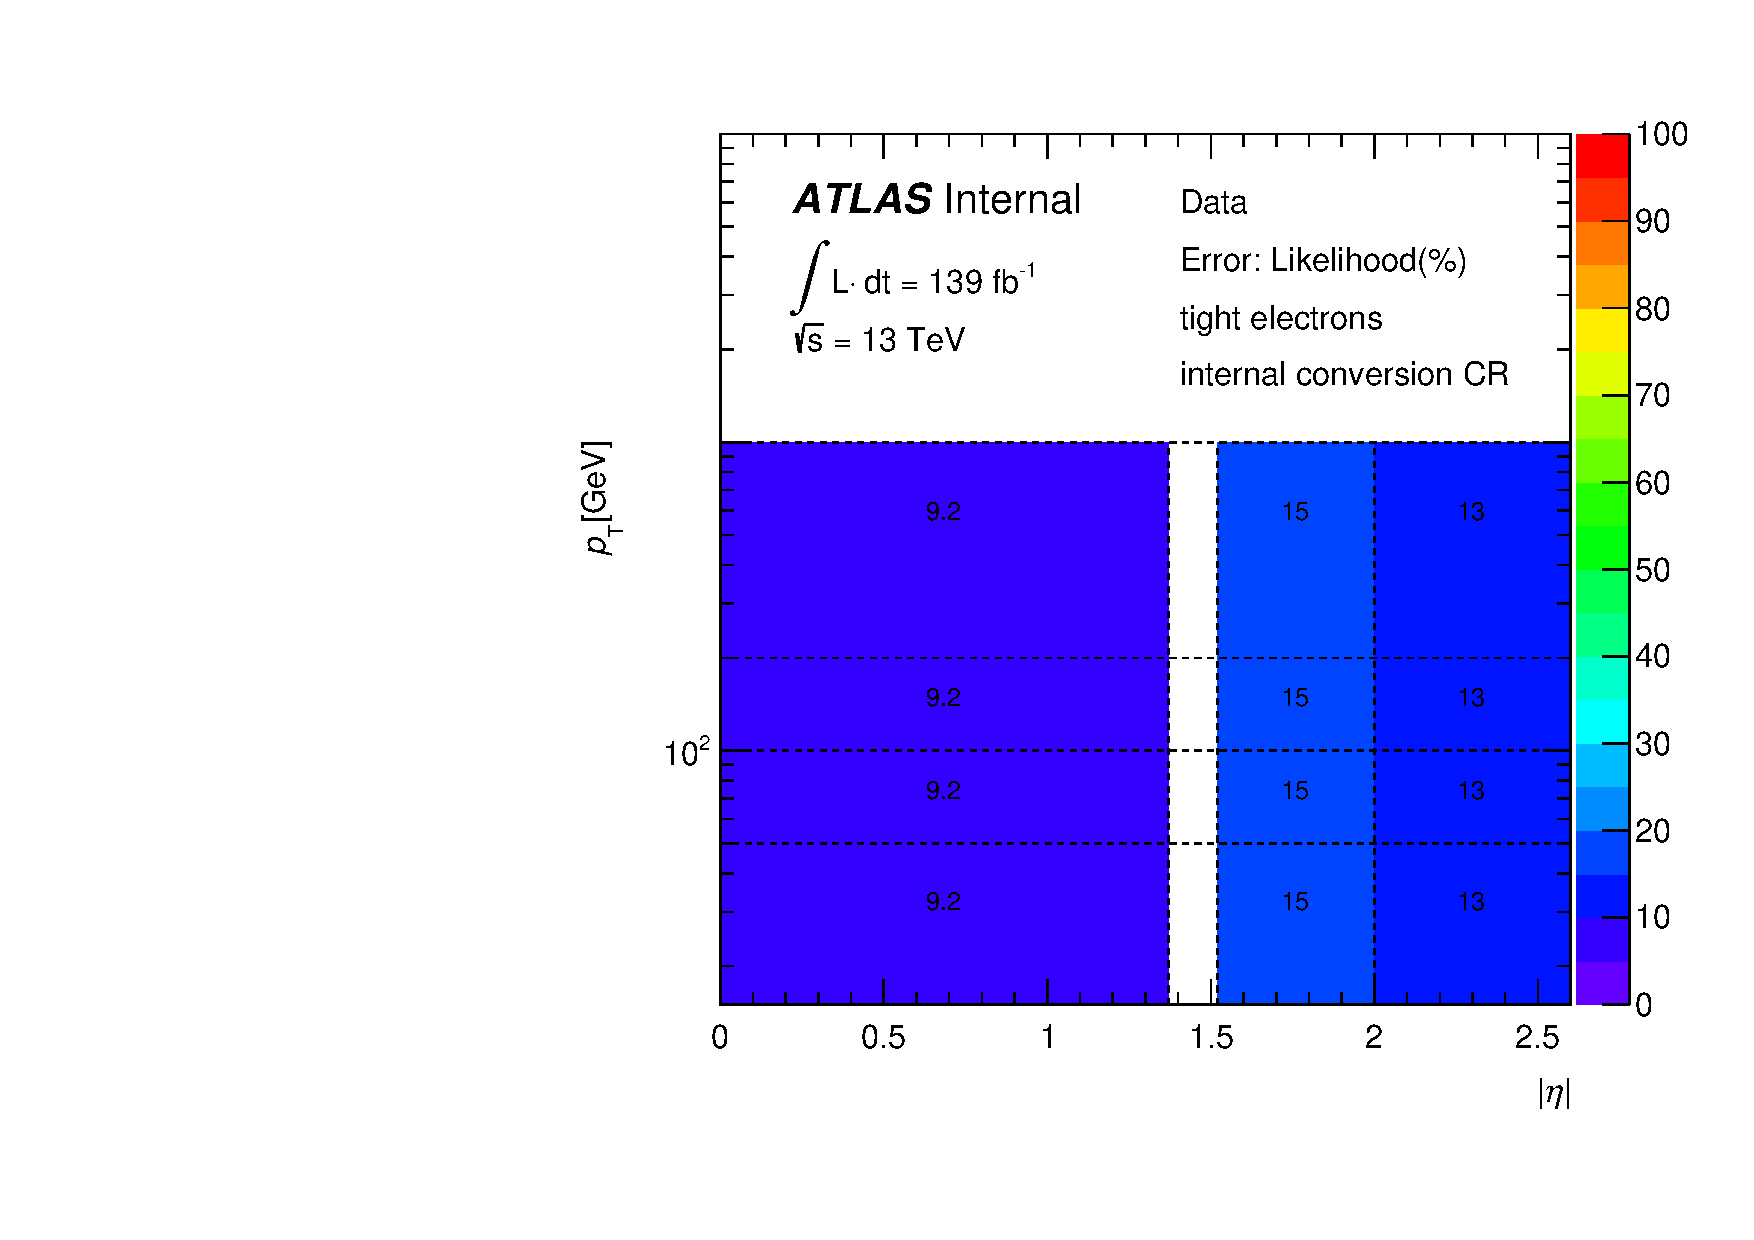
\includegraphics[width=0.45\textwidth]{figures/qmisid/syst_Data_Likelihood_tight_intcr}
  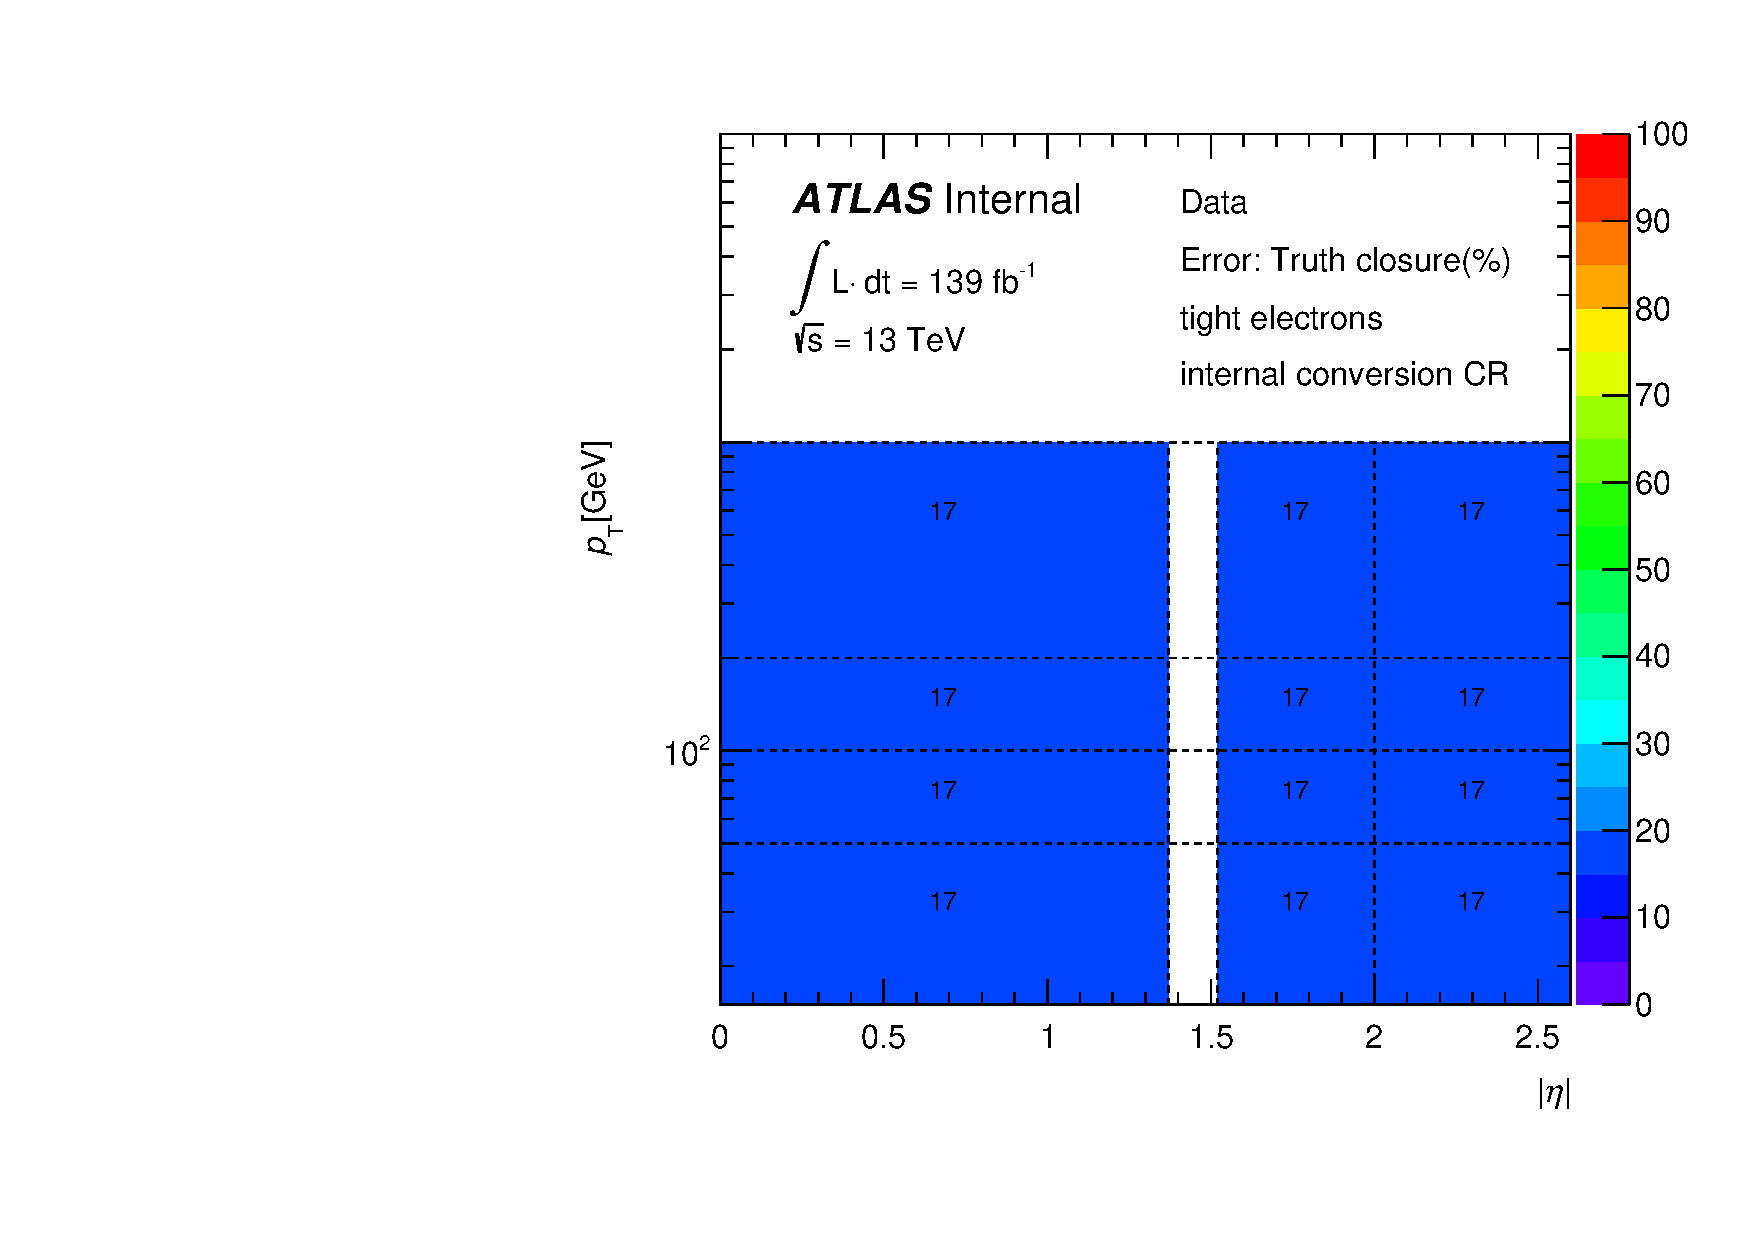
\includegraphics[width=0.45\textwidth]{figures/qmisid/syst_Data_Truthclosure_tight_intcr}\\
  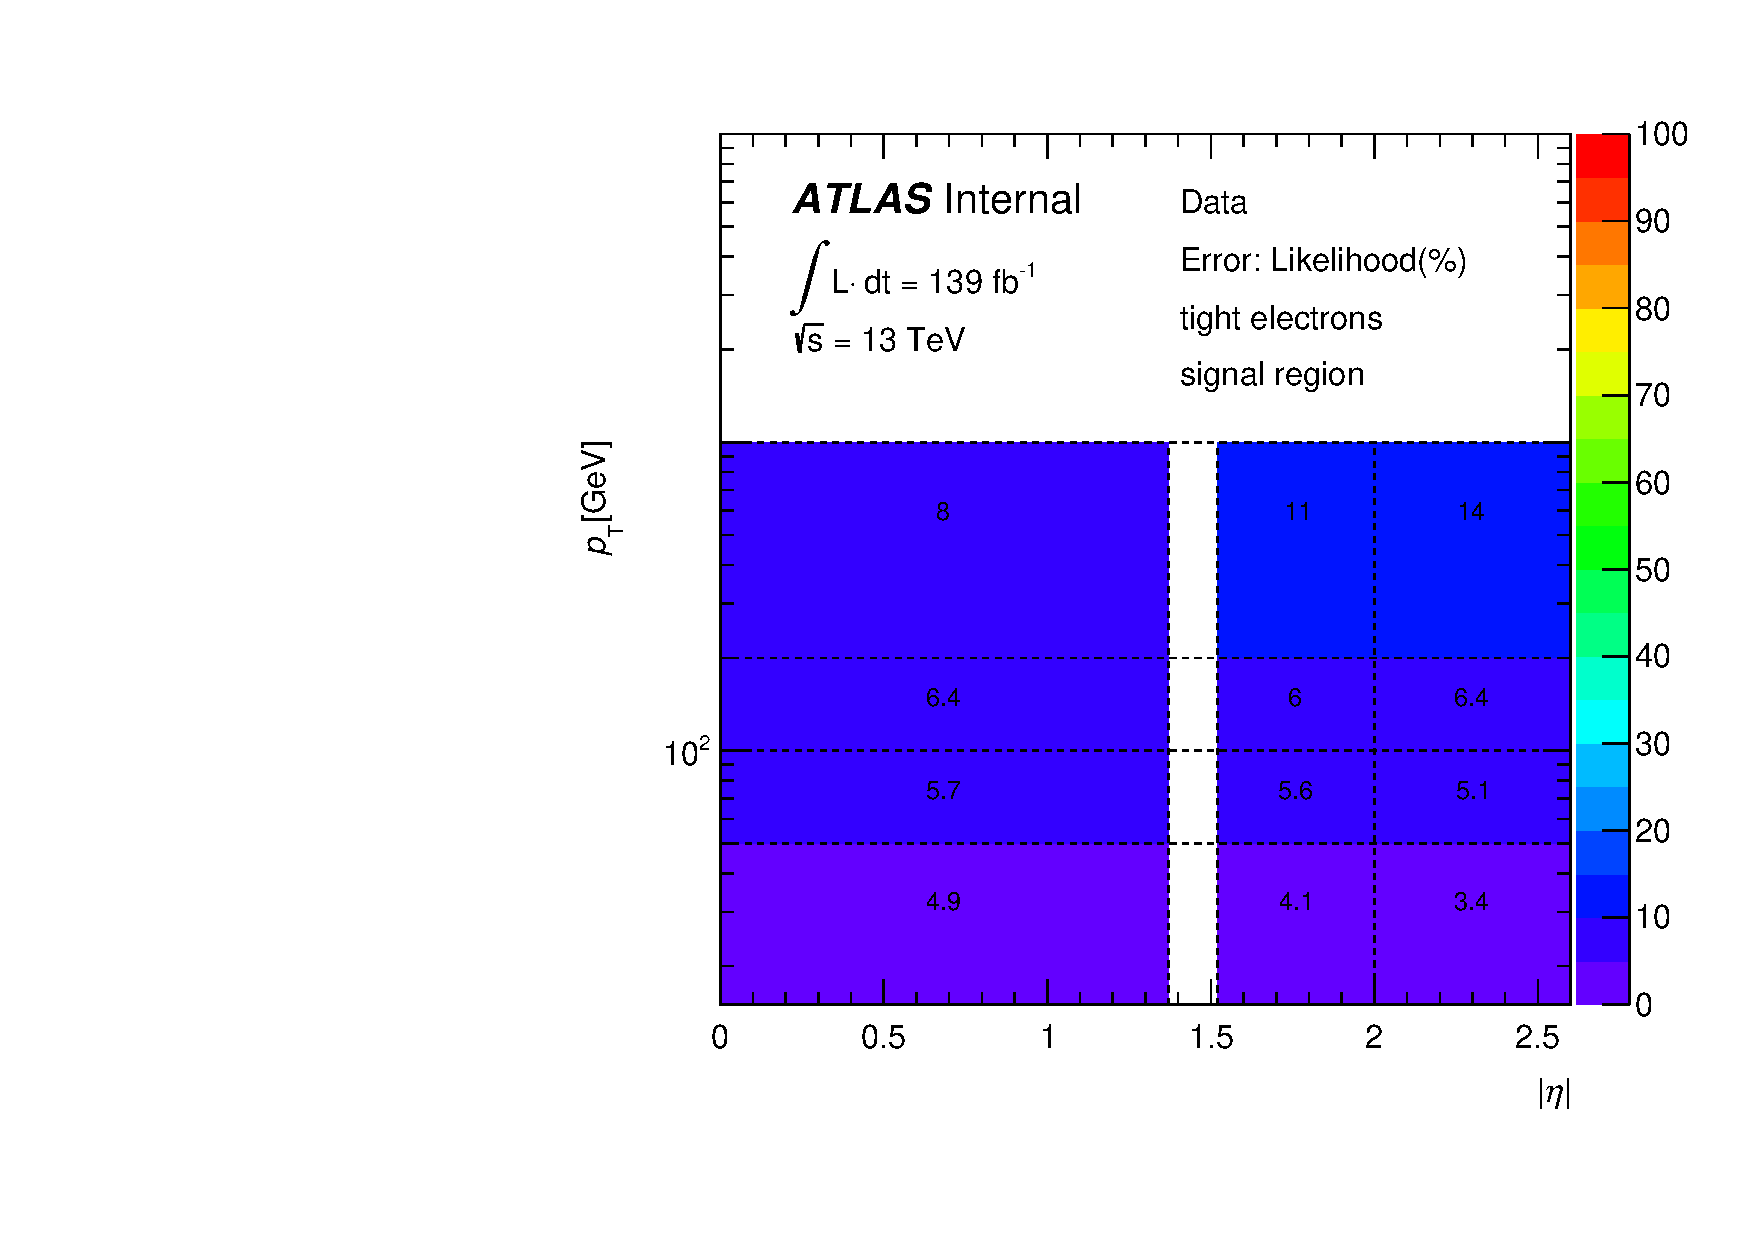
\includegraphics[width=0.45\textwidth]{figures/qmisid/syst_Data_Likelihood_tight_sr}
  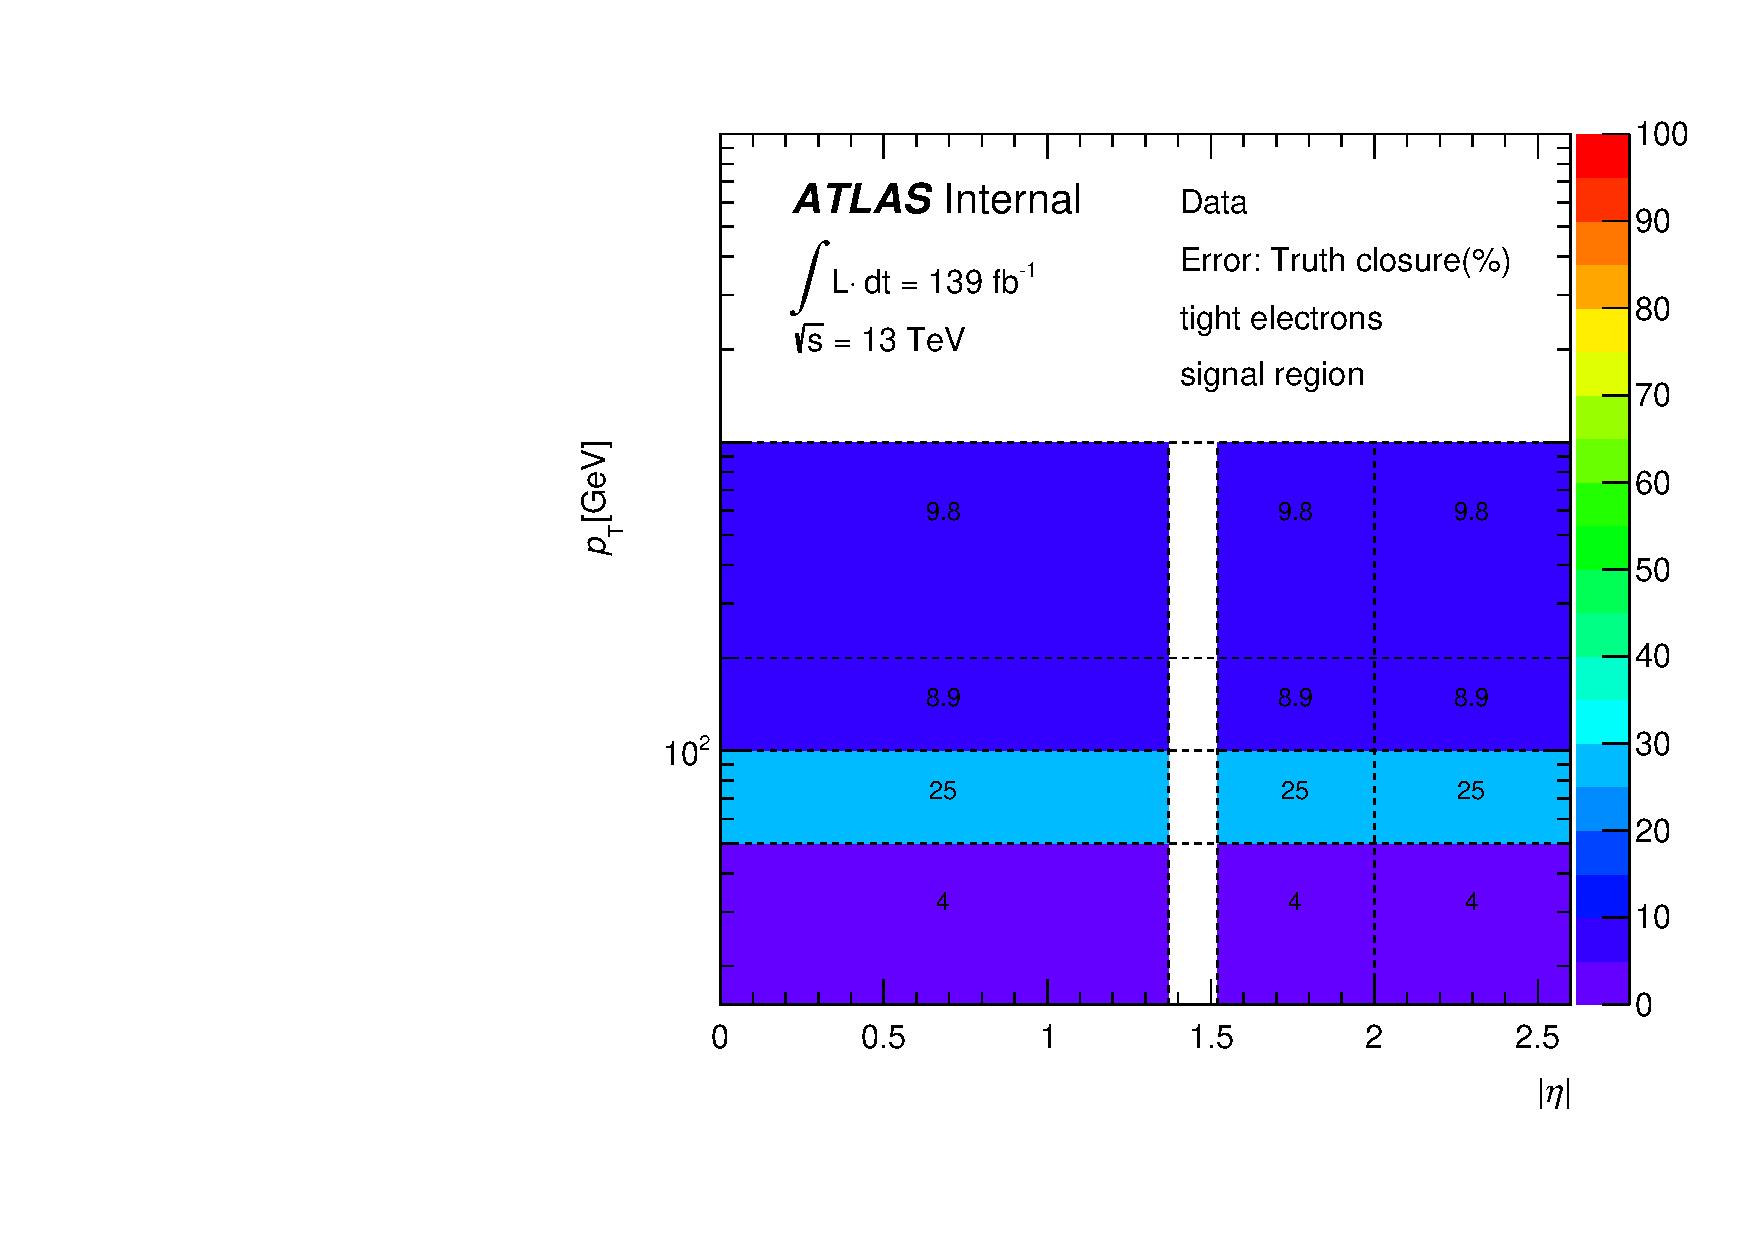
\includegraphics[width=0.45\textwidth]{figures/qmisid/syst_Data_Truthclosure_tight_sr}
  \caption{ \label{fig:QMisID:systa} Left: systematic uncertainty (\%), introduced from the statistical size of the control 
            region of the data that is used in the likelihood method, in bins of $|\eta|$ and $\pT$. Right: systematic uncertainty 
            (\%), introduced from the comparison of rates obtained from simulated $Z\rightarrow ee$ events with the likelihood 
            method to truth-based rates.}
  \end{center}
\end{figure}

\begin{figure}[p!]
  \begin{center}
  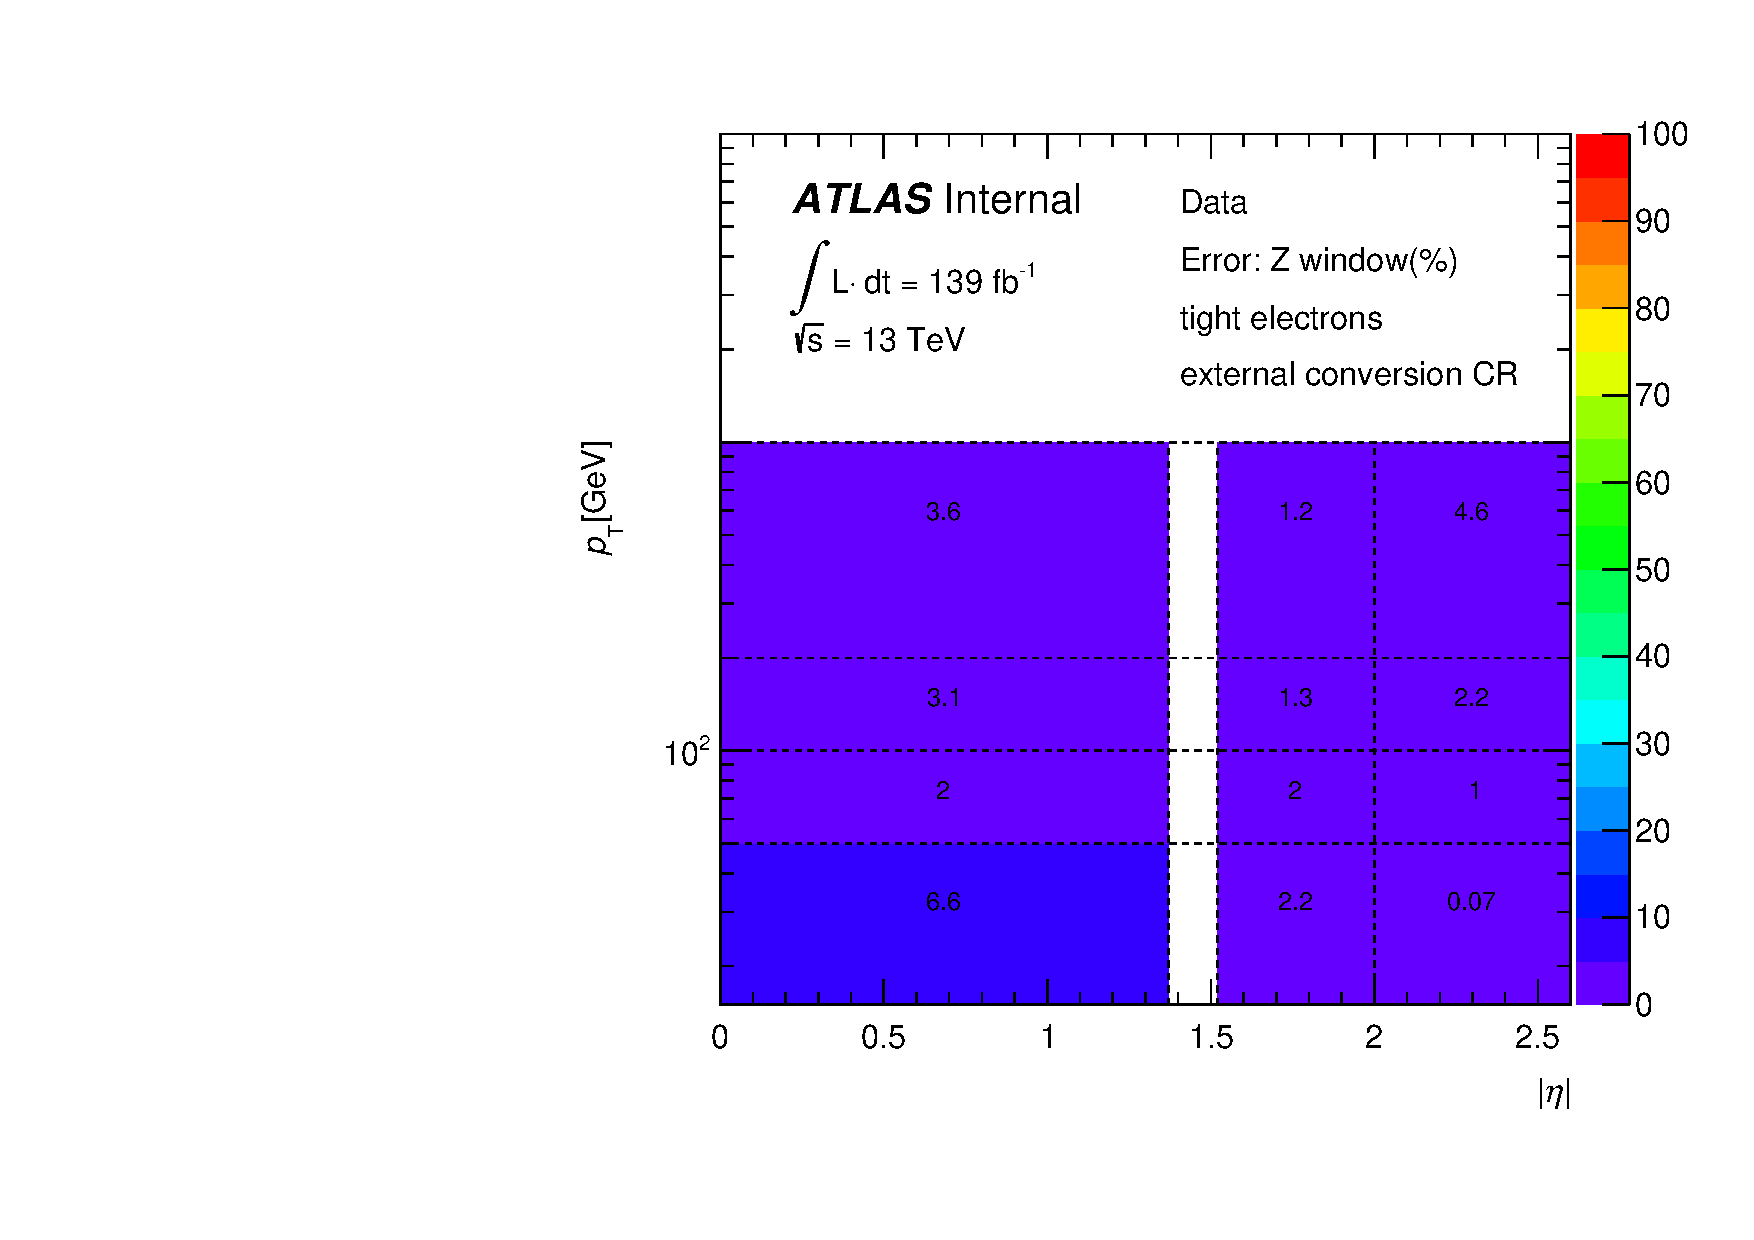
\includegraphics[width=0.45\textwidth]{figures/qmisid/syst_Data_Zwindow_tight_extcr}
  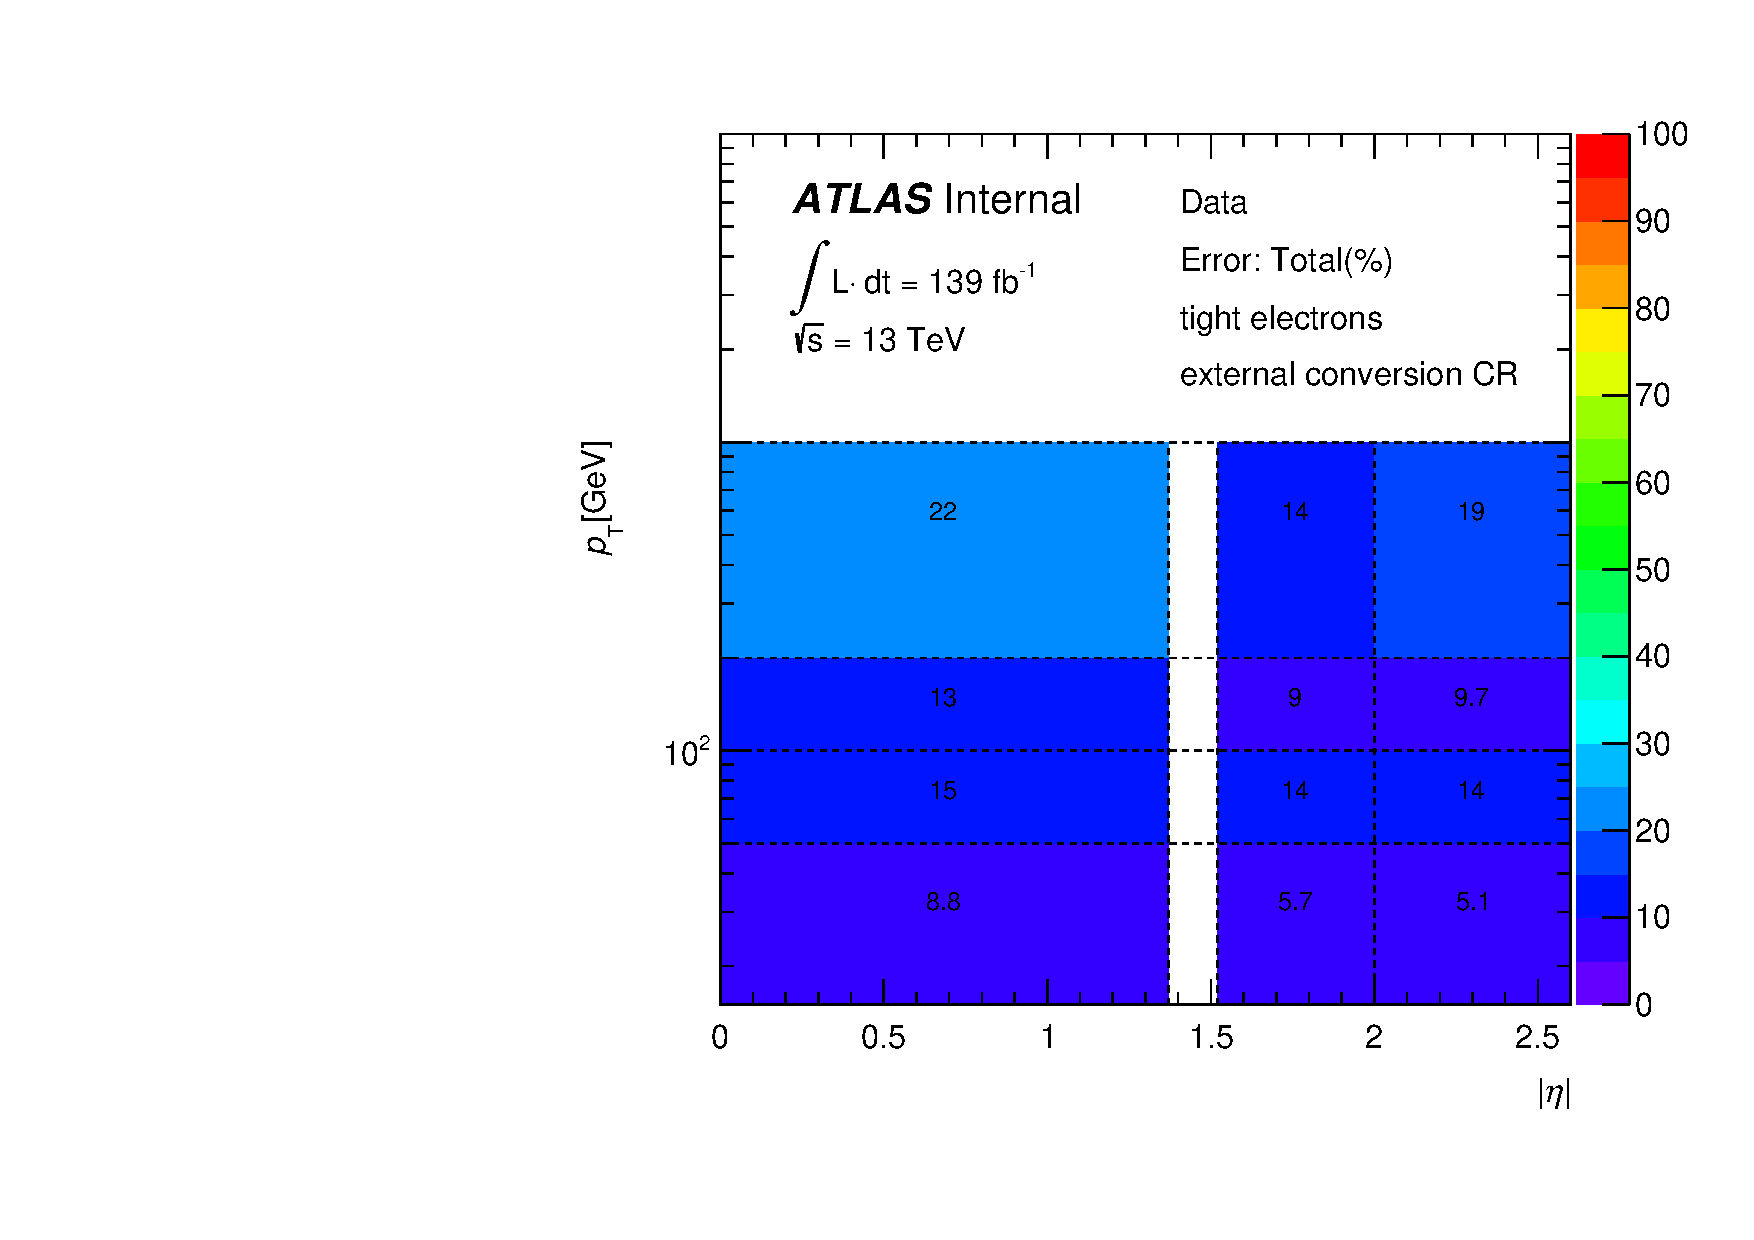
\includegraphics[width=0.45\textwidth]{figures/qmisid/syst_Data_Total_tight_extcr}\\
  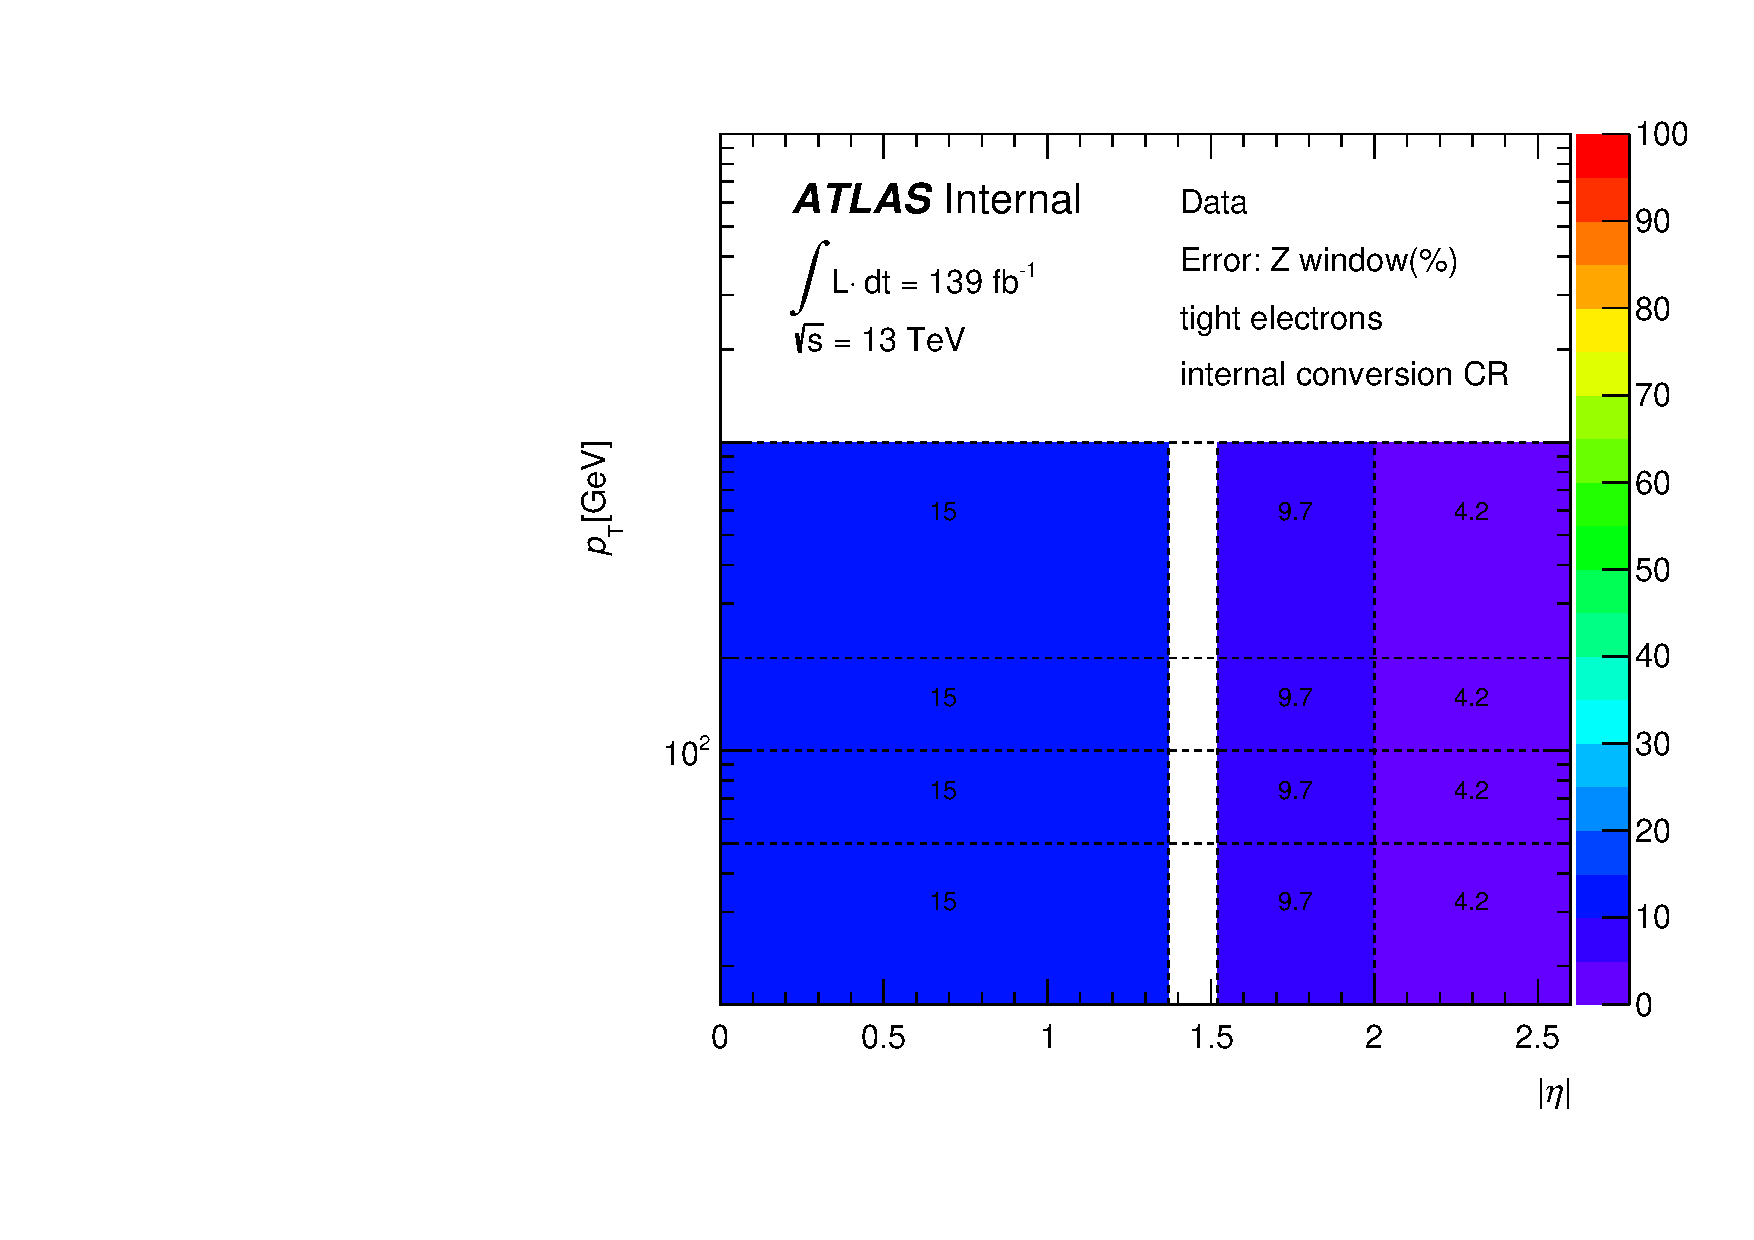
\includegraphics[width=0.45\textwidth]{figures/qmisid/syst_Data_Zwindow_tight_intcr}
  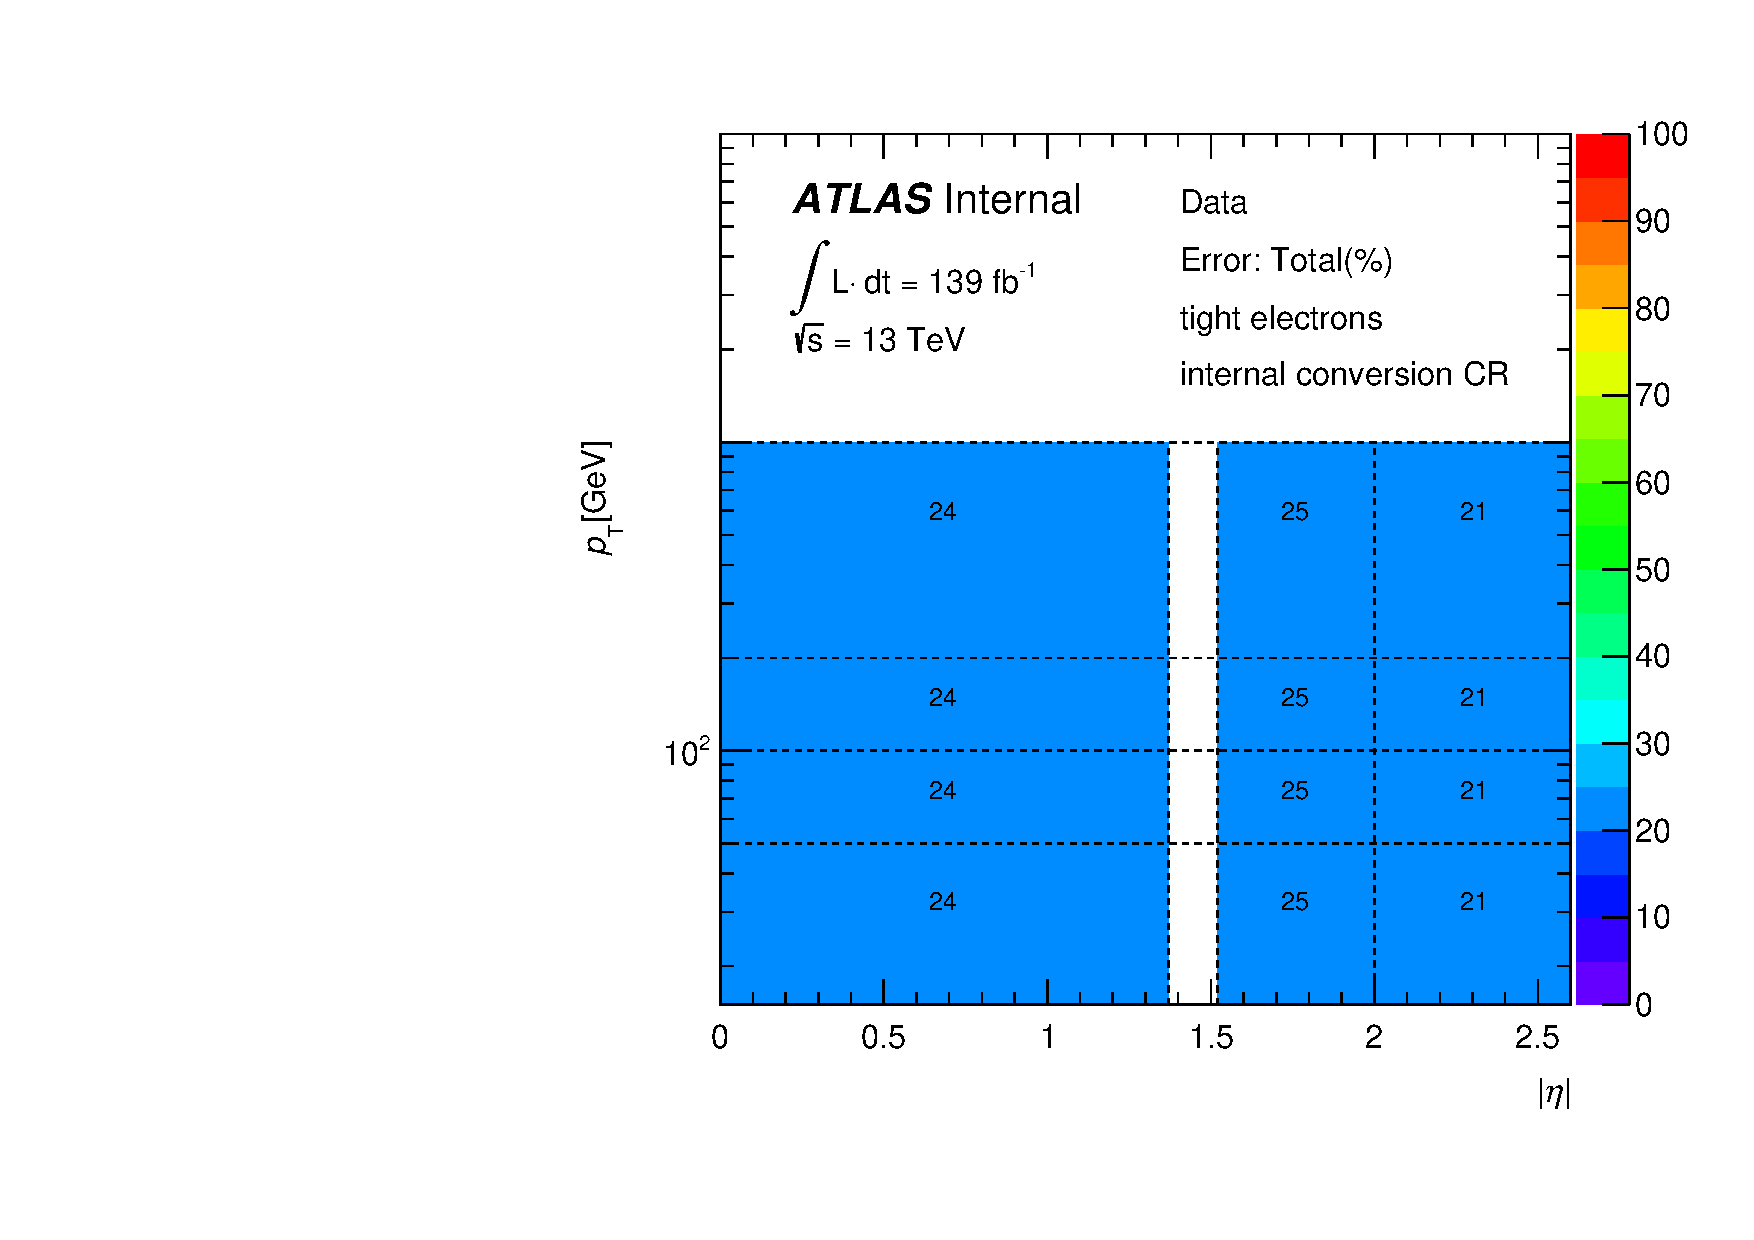
\includegraphics[width=0.45\textwidth]{figures/qmisid/syst_Data_Total_tight_intcr}\\
  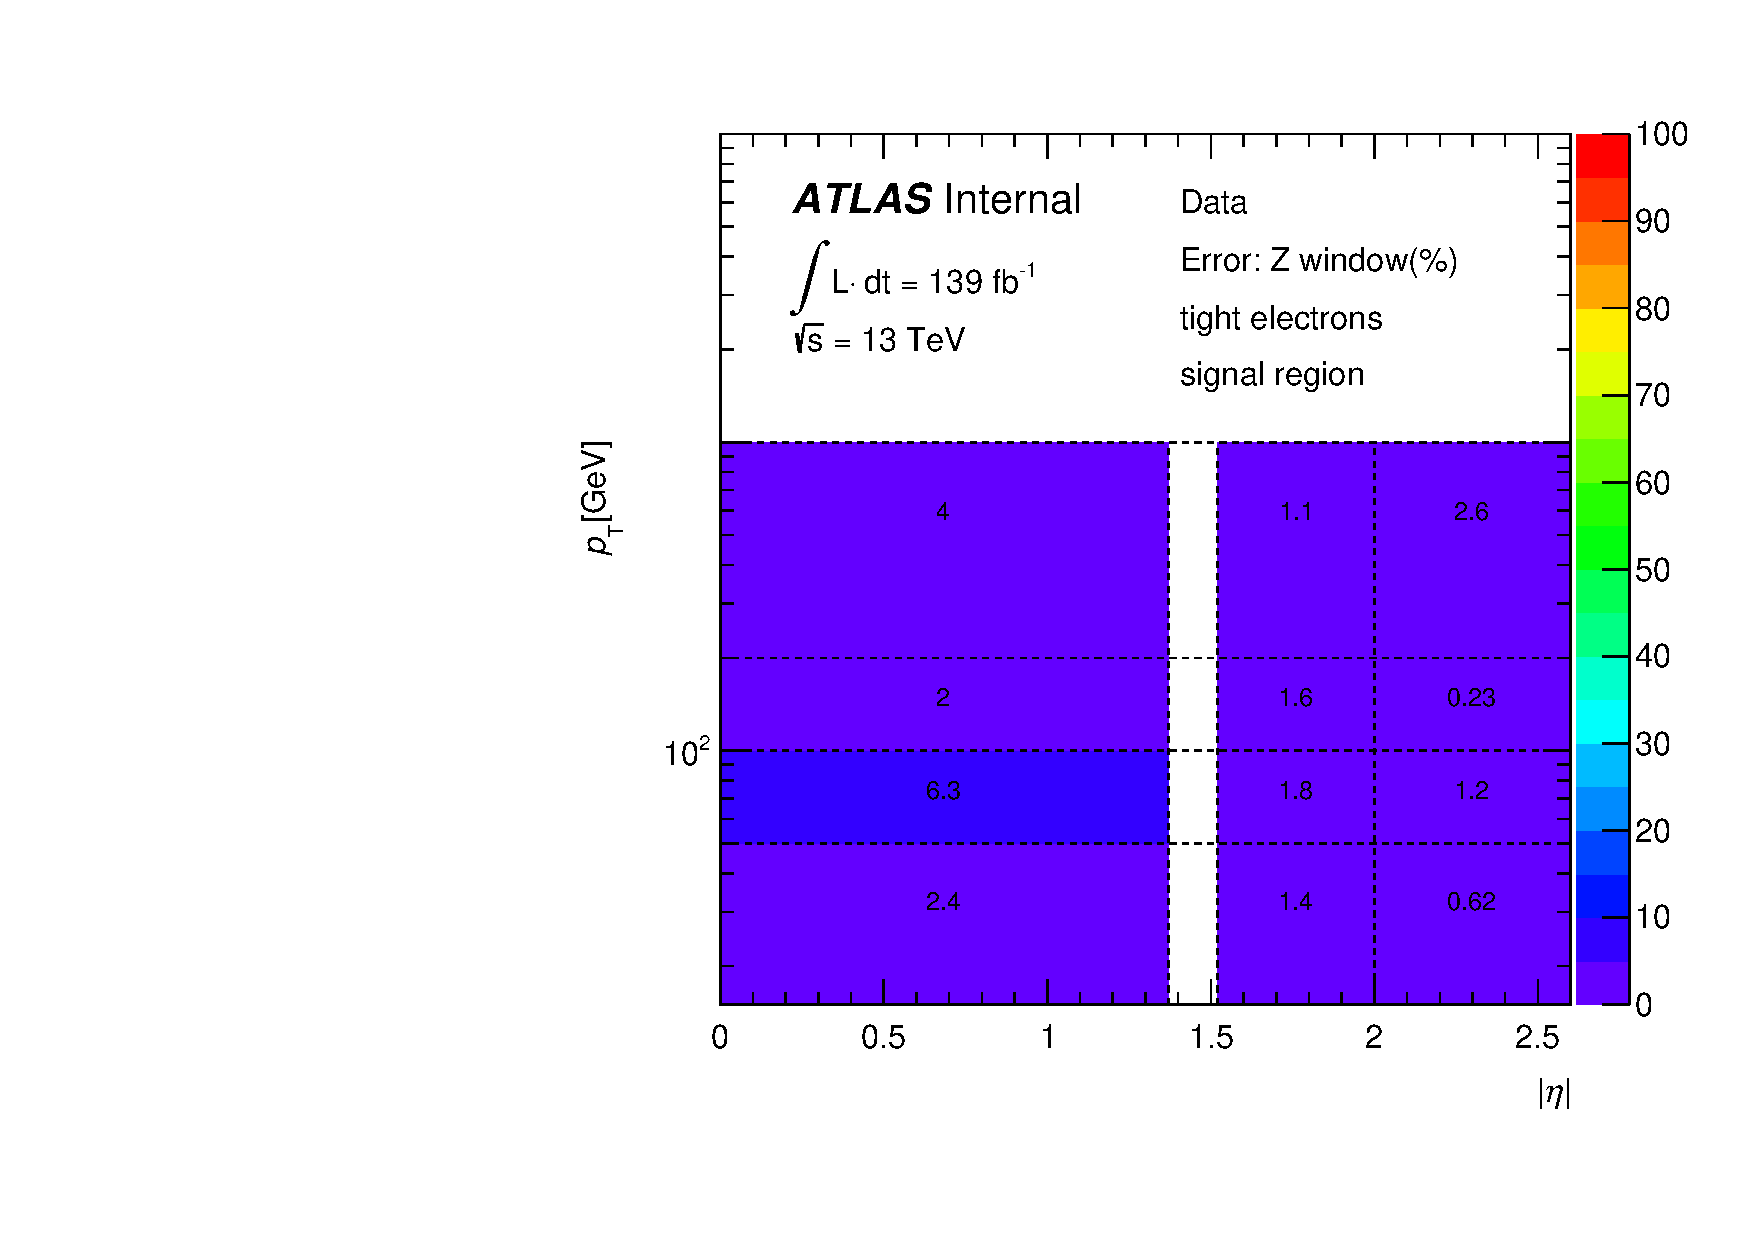
\includegraphics[width=0.45\textwidth]{figures/qmisid/syst_Data_Zwindow_tight_sr}
  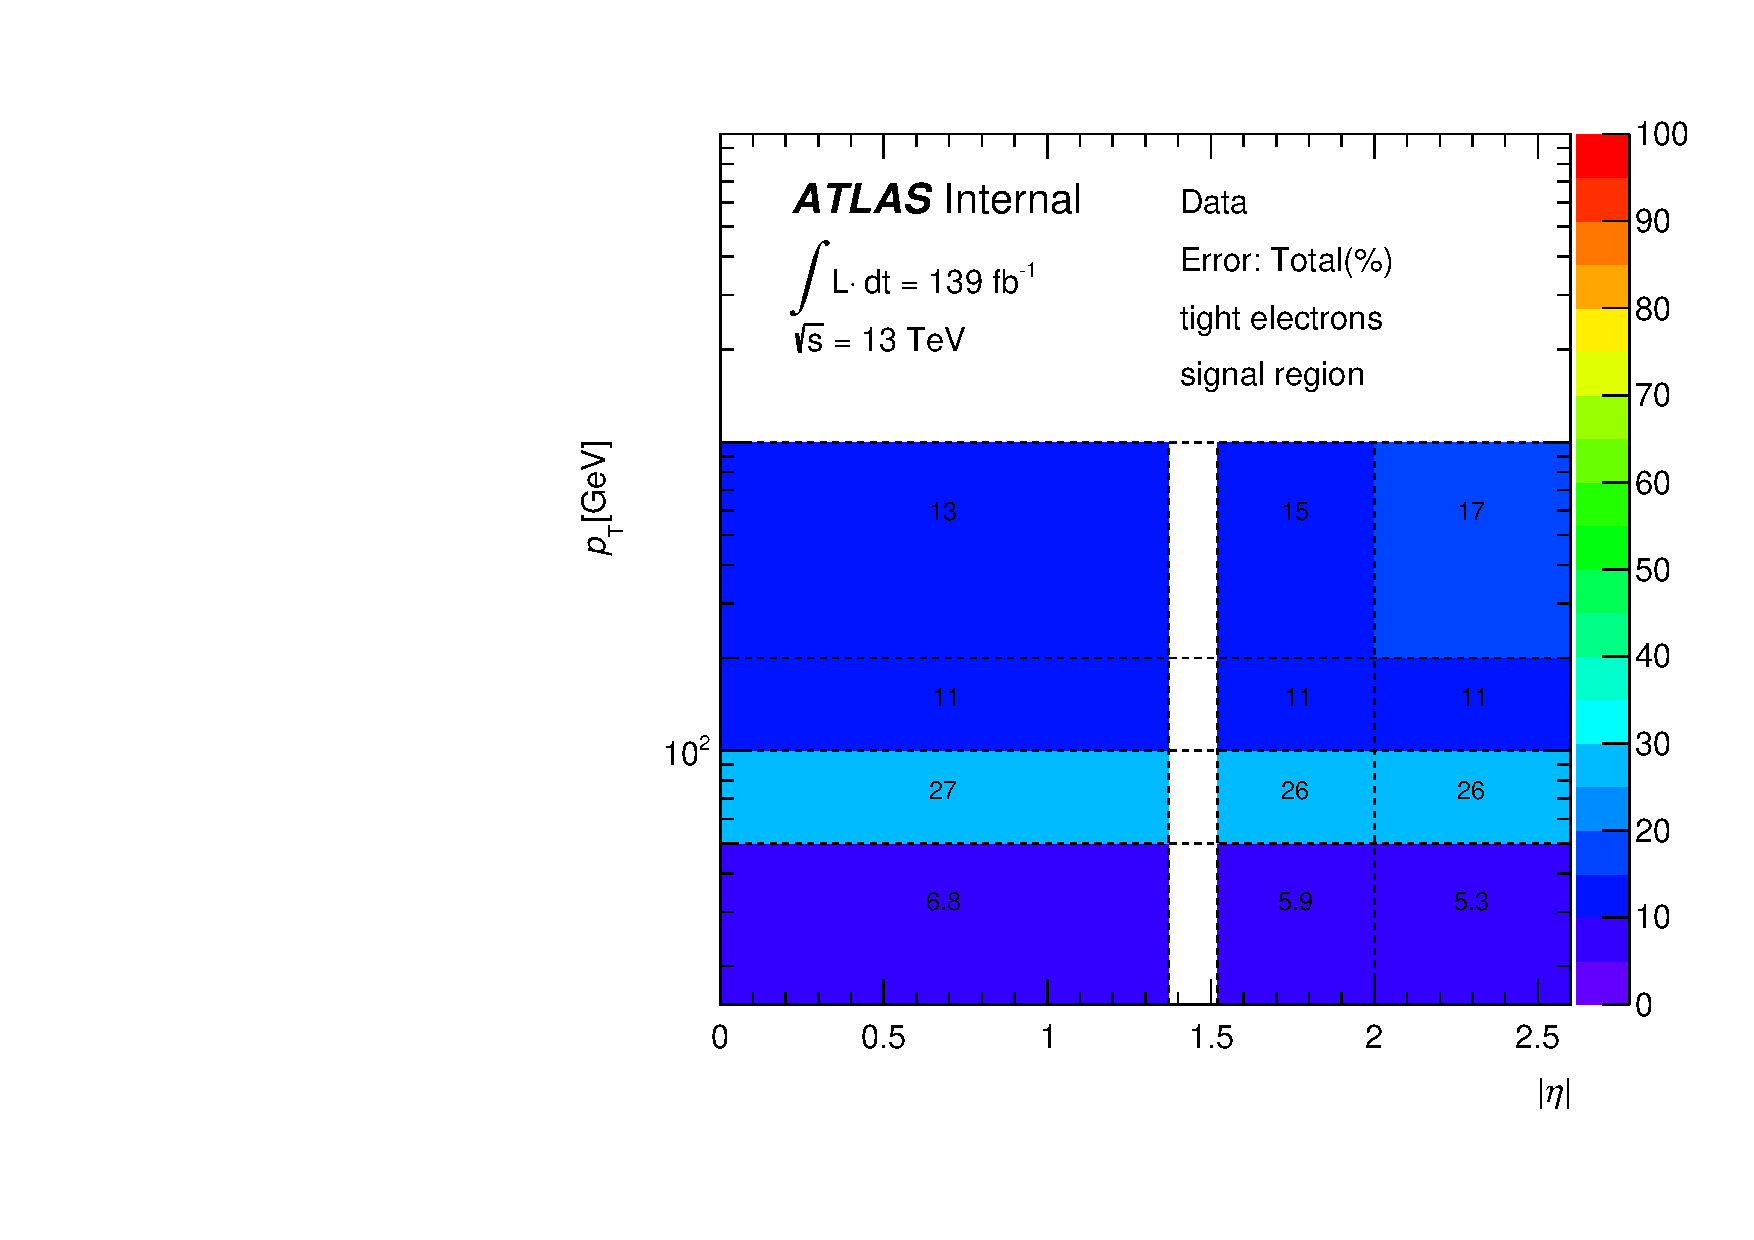
\includegraphics[width=0.45\textwidth]{figures/qmisid/syst_Data_Total_tight_sr}
  \caption{ \label{fig:QMisID:systb} Left: systematic uncertainty (\%), introduced from the variation of the $m_{Z}$ window
  (and its sidebands) that is used to obtain the rates, in bins of $|\eta|$ and $\pT$. Right: Total systematic uncertainty (\%).}
  \end{center}
\end{figure}

%~~~~~~~~~~~~~~~~~~~~~~~~~~~~~~~~~~~
\subsubsection{Closure test}
\label{Sec:closure}
%~~~~~~~~~~~~~~~~~~~~~~~~~~~~~~~~~~~

The rates are validated by comparing the estimated number of same-sign $ee$ events (using the QMisID rates on
opposite-sign events) to the measured number of same-sign events. In order to increase the statistical
precision, this test is performed without any requirement regarding the number of jets. 
Figure\,\ref{fig:clData}, shows the expected distribution of $m_{ee}$ in the data, compared to the observation
(the latter also contains contributions from non-prompt electrons). 
After subtracting the non-prompt electron background using the sidebands, the
measured number of same-sign events in the $m_{Z}$ window is found to be 6474
(1076) for events with at least 1 jet (3 jets) while the expectation is
$6951 \pm 1024$ ($1156 \pm 95$). The $\pT$ distribution (within the $m_{Z}$ window) is also presented 
in figure\,\ref{fig:clData}, showing agreement between the measurement and the prediction, which however begins 
to deteriorate in the very high $\pT$ region, due to the fact that the region above 200\,GeV is described by an 
inclusive QmisID rate.

The respective comparison with $Z$+jets MC (in which the non-prompt contribution is removed using the truth 
information) is shown in figure\,\ref{fig:clMC}.

\begin{figure}[htb!]
\centering
  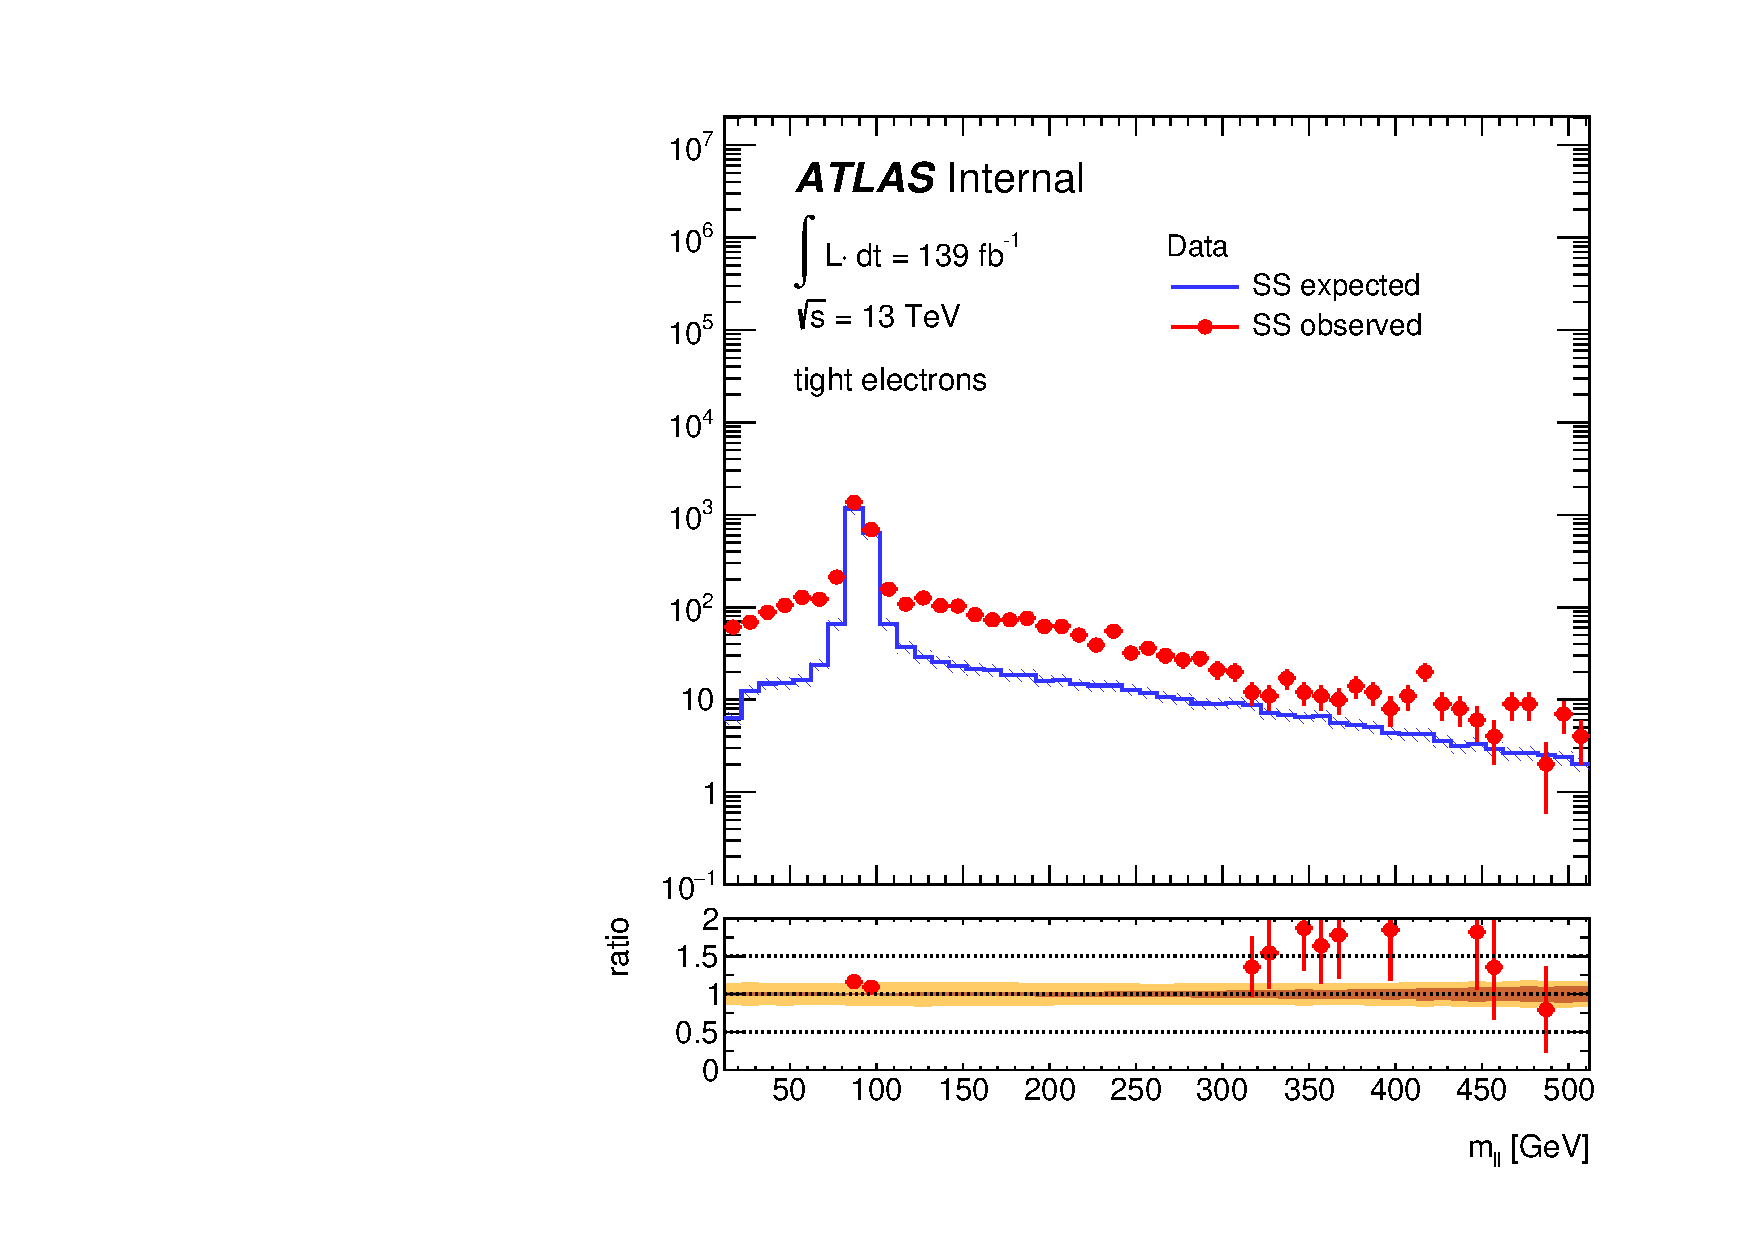
\includegraphics[width=0.45\textwidth]{figures/qmisid/valid_MlltightData}
  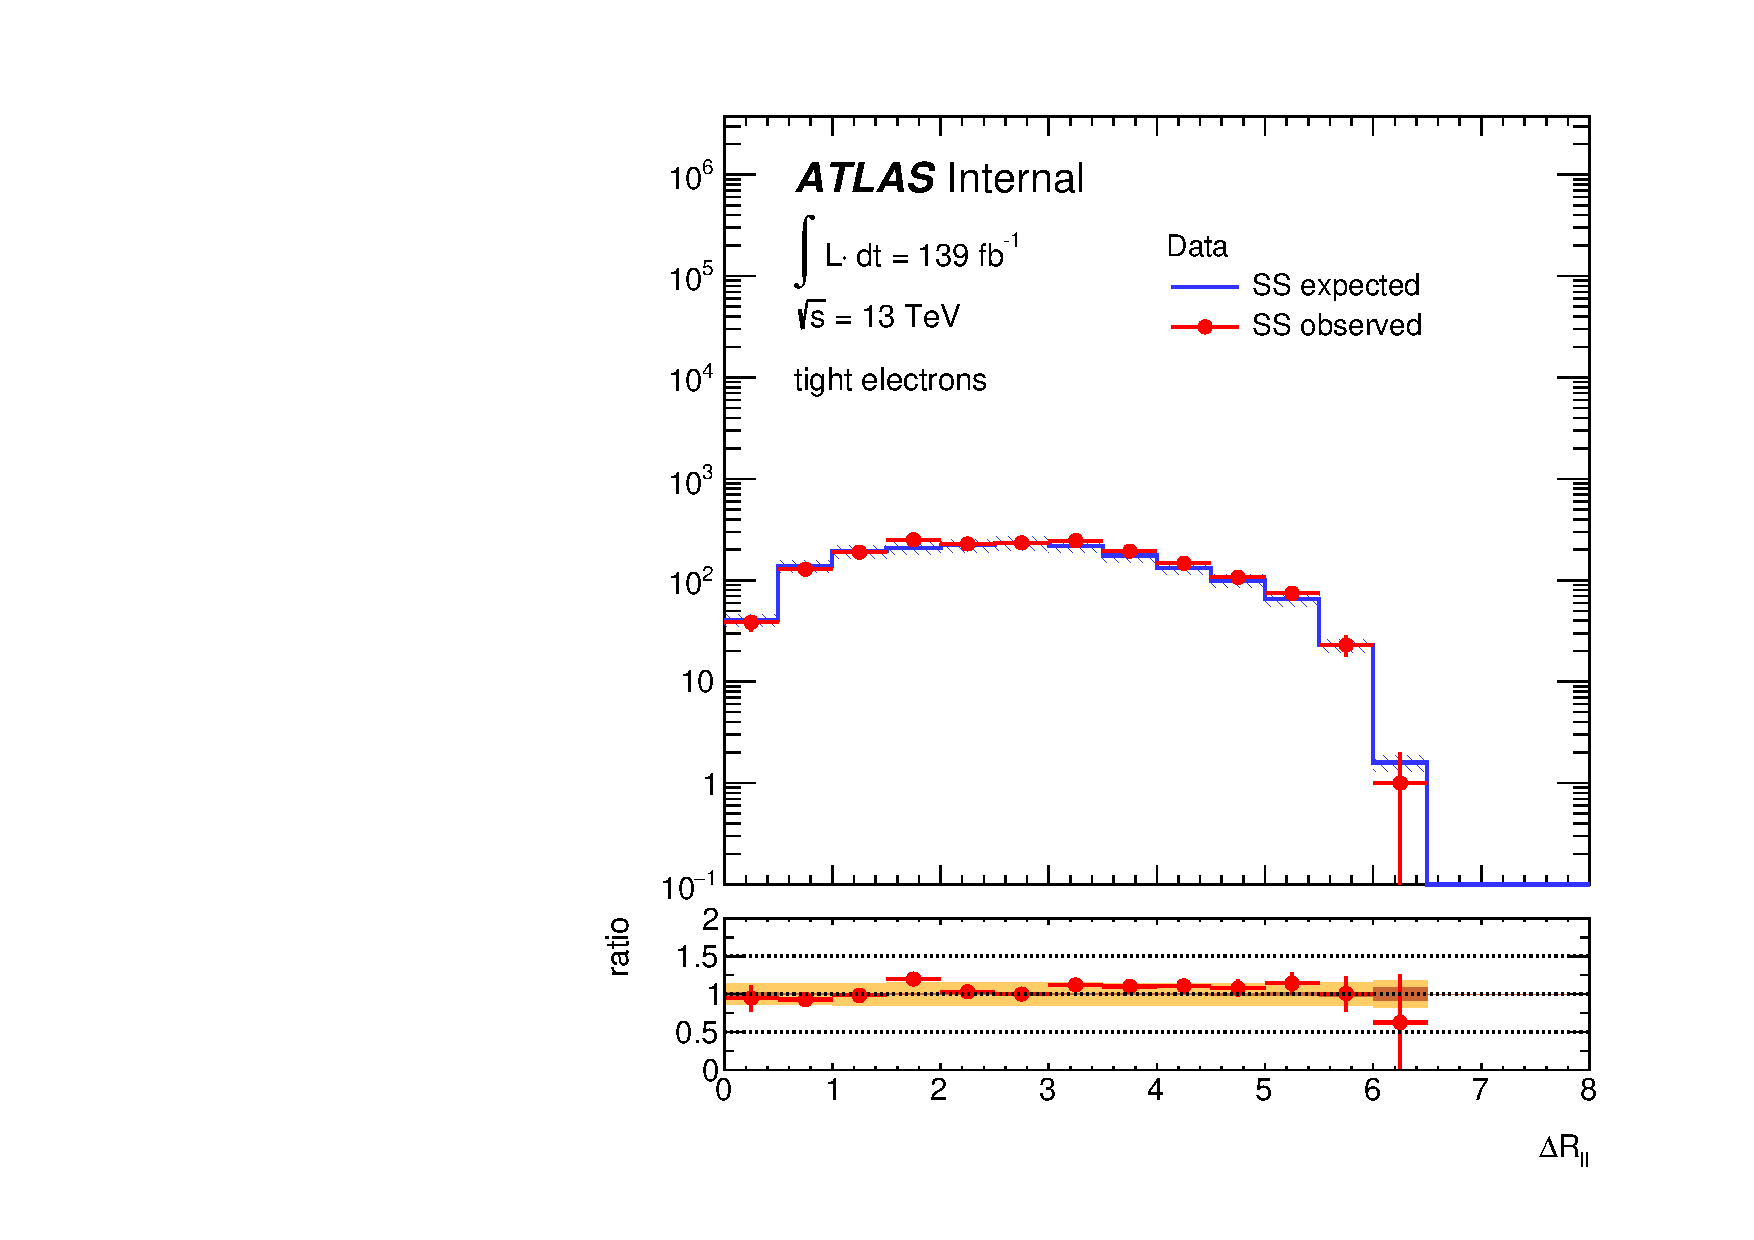
\includegraphics[width=0.45\textwidth]{figures/qmisid/valid_DRlltightData}\\
  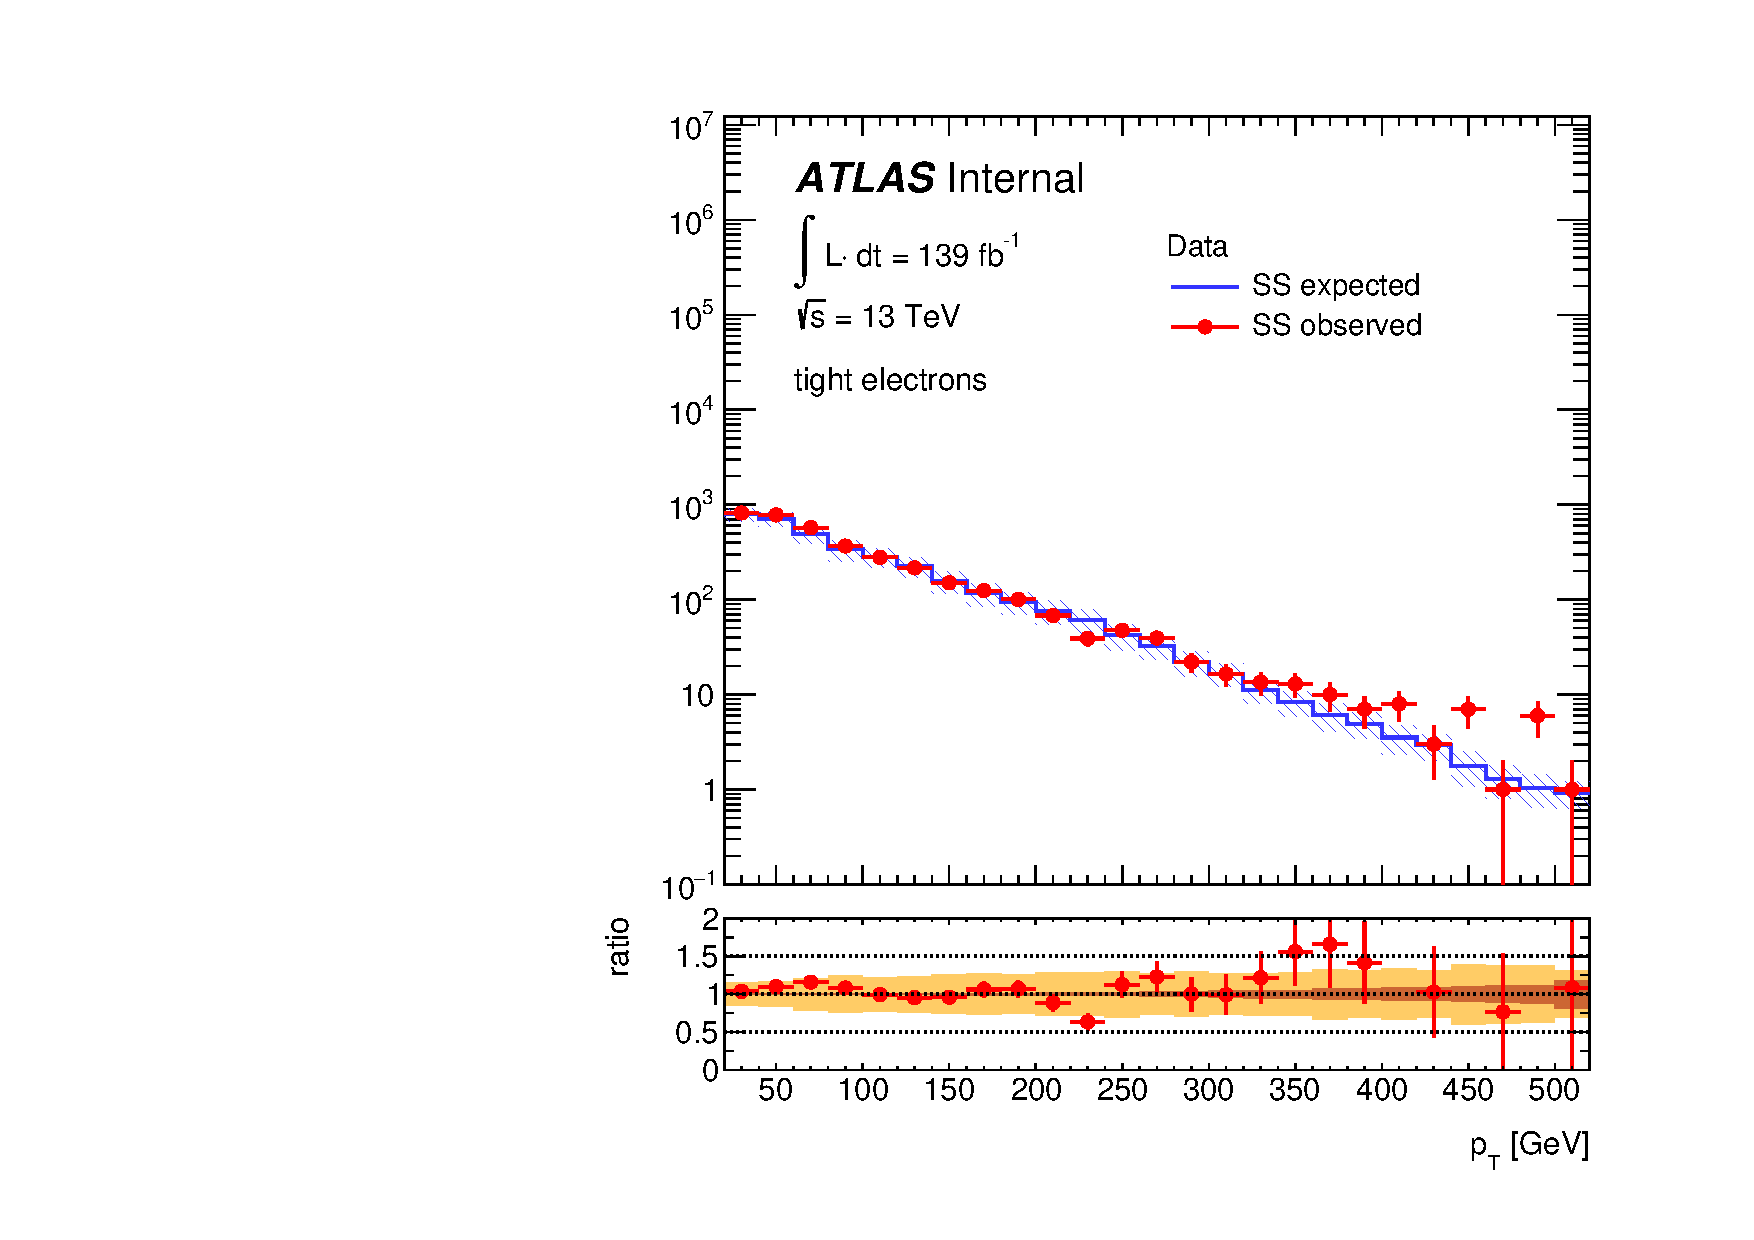
\includegraphics[width=0.45\textwidth]{figures/qmisid/valid_PttightData}
  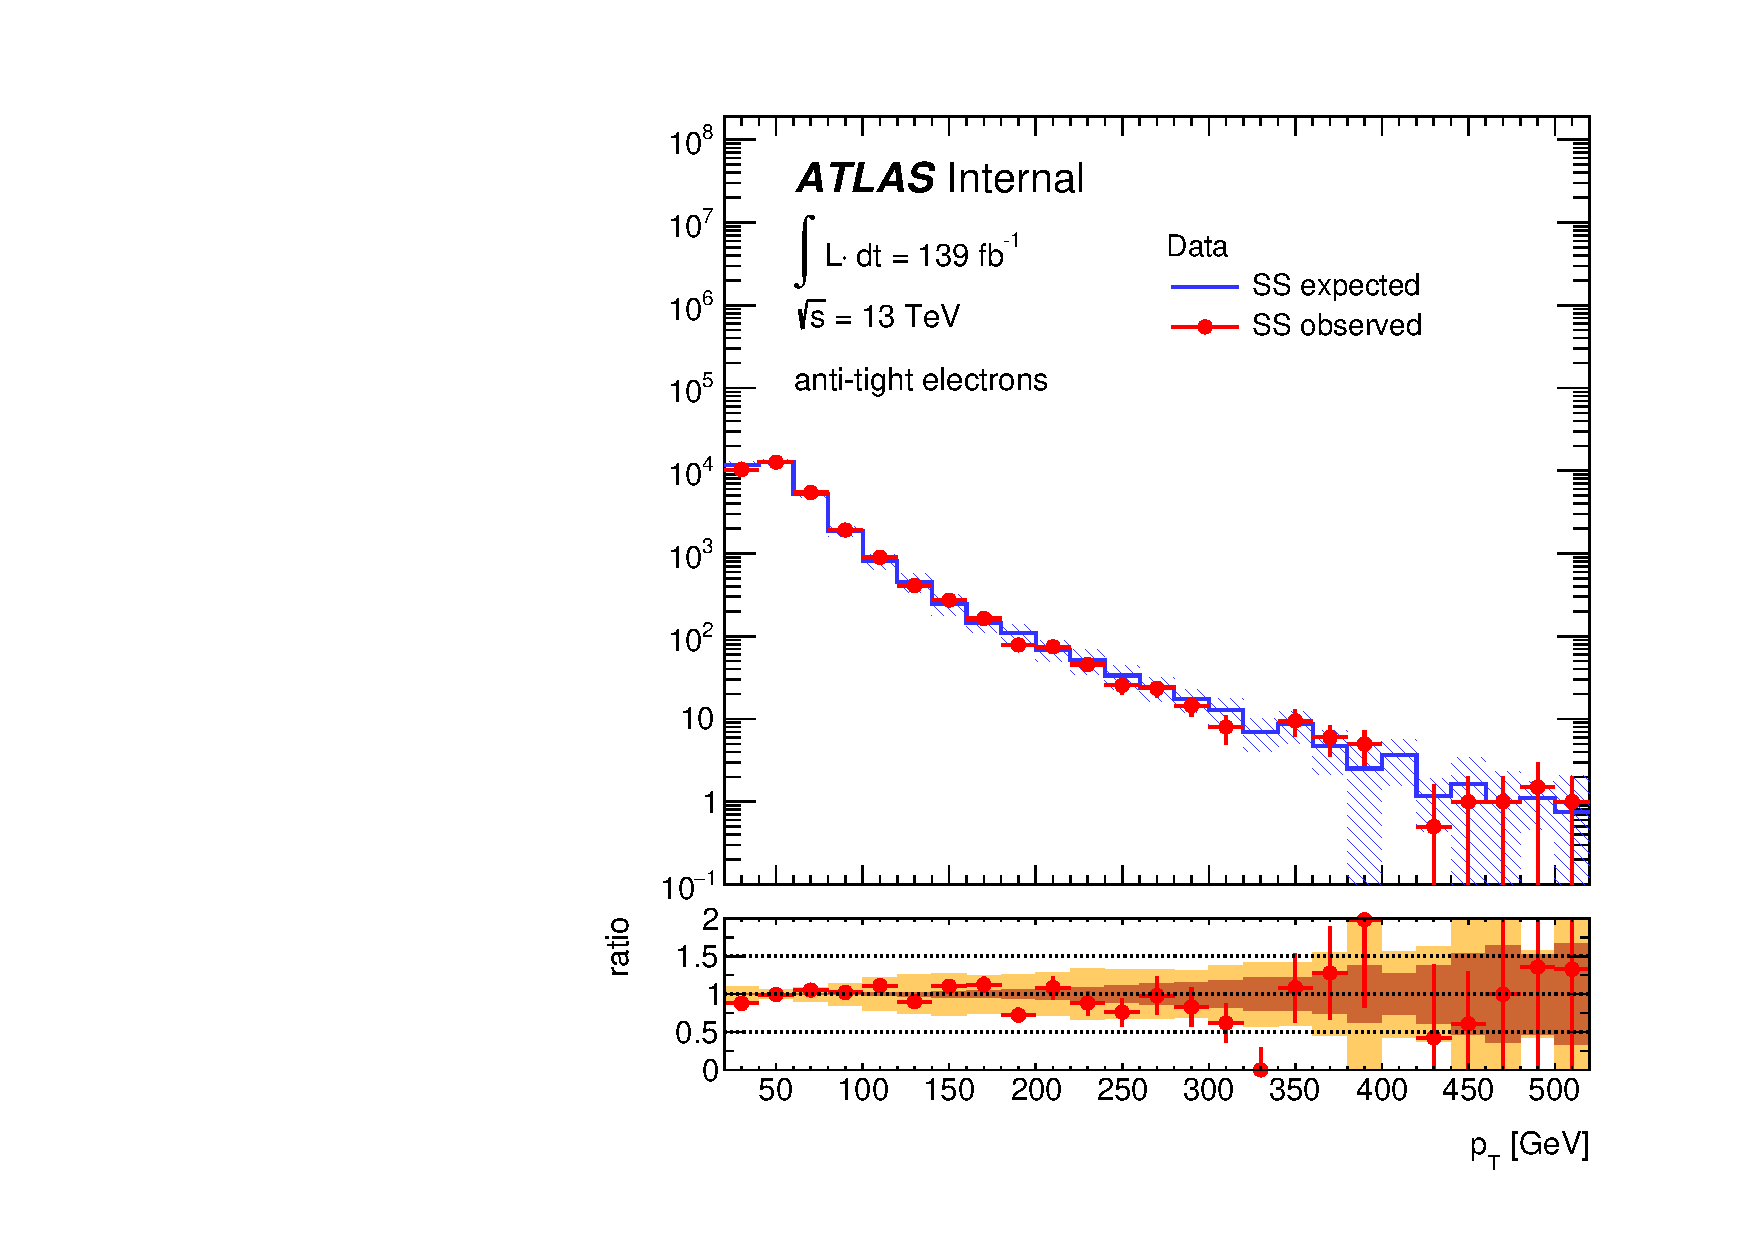
\includegraphics[width=0.45\textwidth]{figures/qmisid/valid_PtatightData}\\
  \caption{Comparison between the expected and observed $m_{ee}$, ${\Delta}R_{ee}$, $pT$ (tight) and $\pT$ (anti-tight) of same-sign electrons.  The dashed bands represent the total (statistical + systematic) uncertainty of the estimation. The comparison is shown for data events. The observed $m_{ee}$ distribution includes the contribution of fake electrons, which are later subtracted by using the sidebands.\label{fig:clData}}
\end{figure}


\begin{figure}[htb!]
\centering
  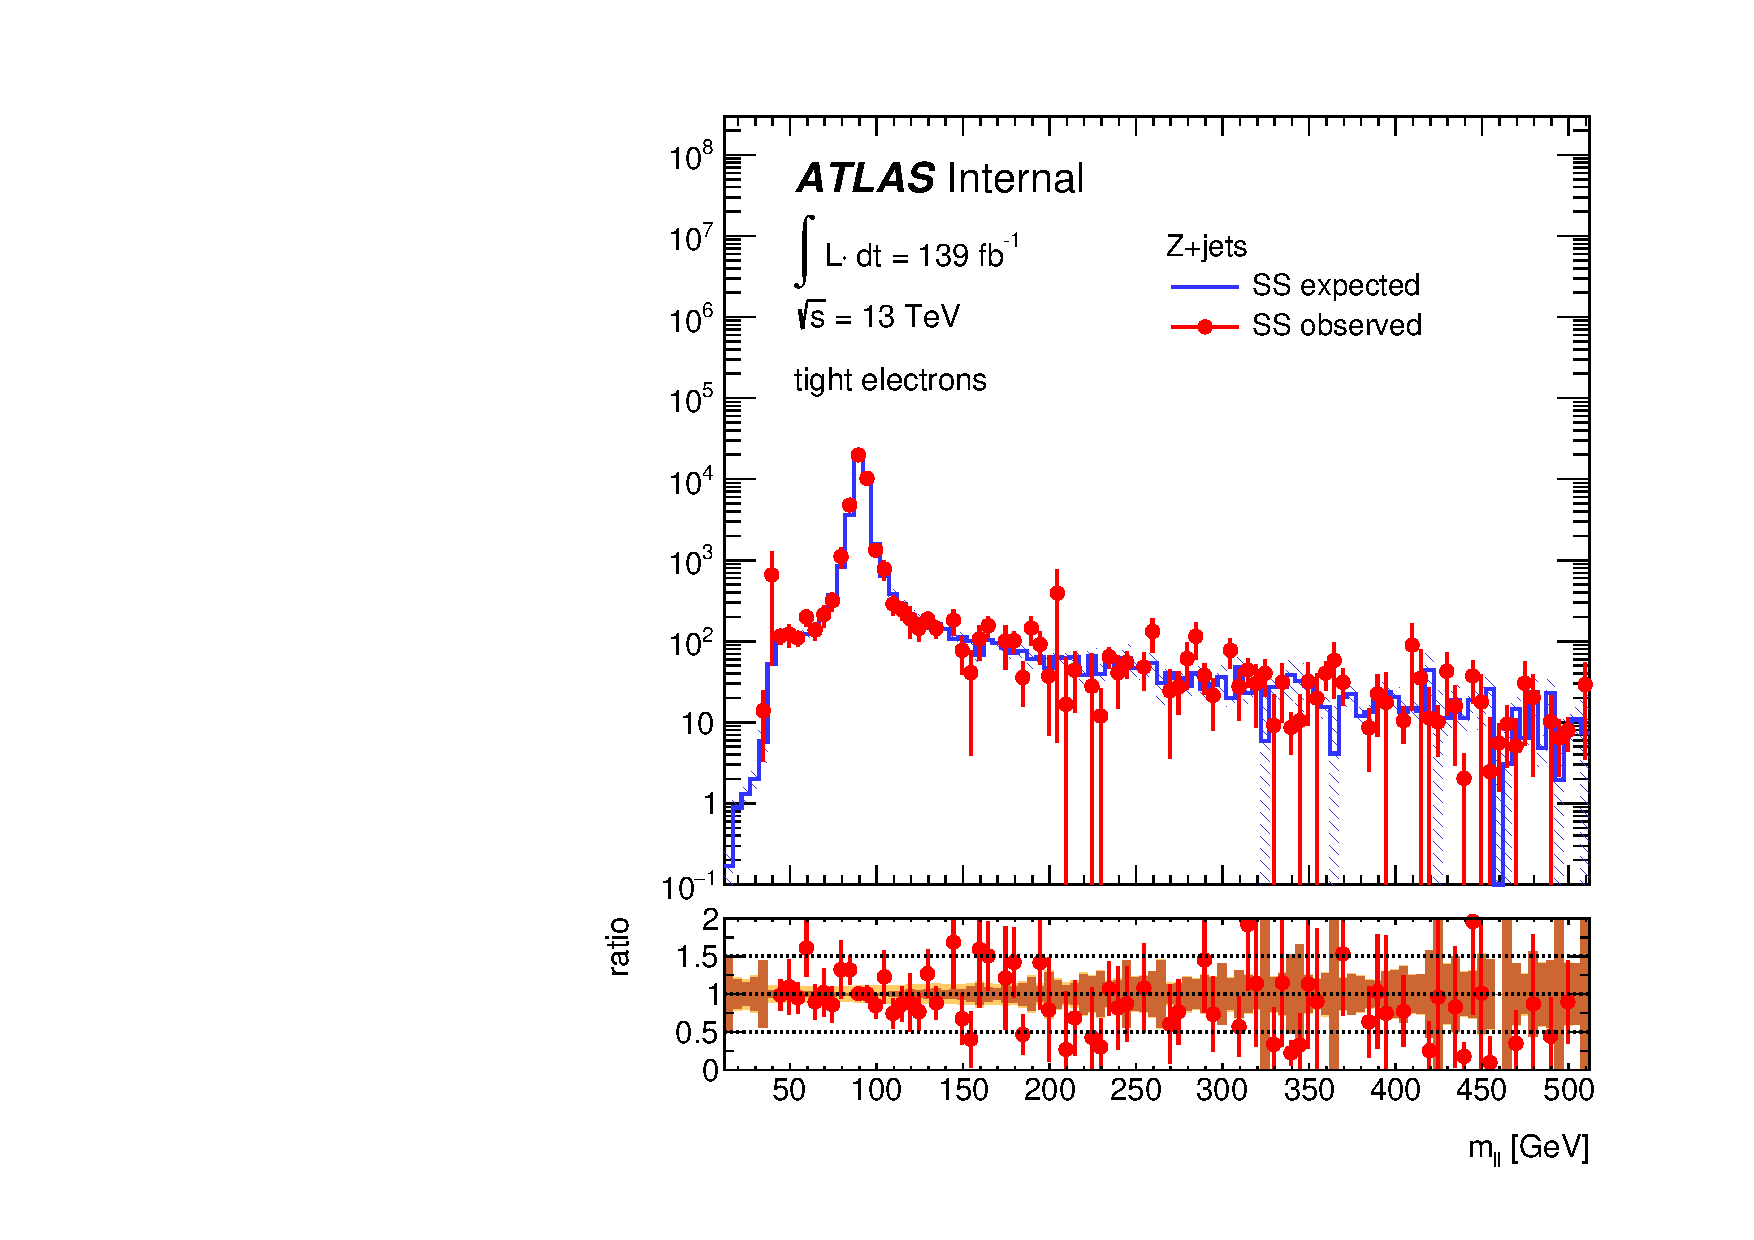
\includegraphics[width=0.45\textwidth]{figures/qmisid/valid_MlltightZ}
  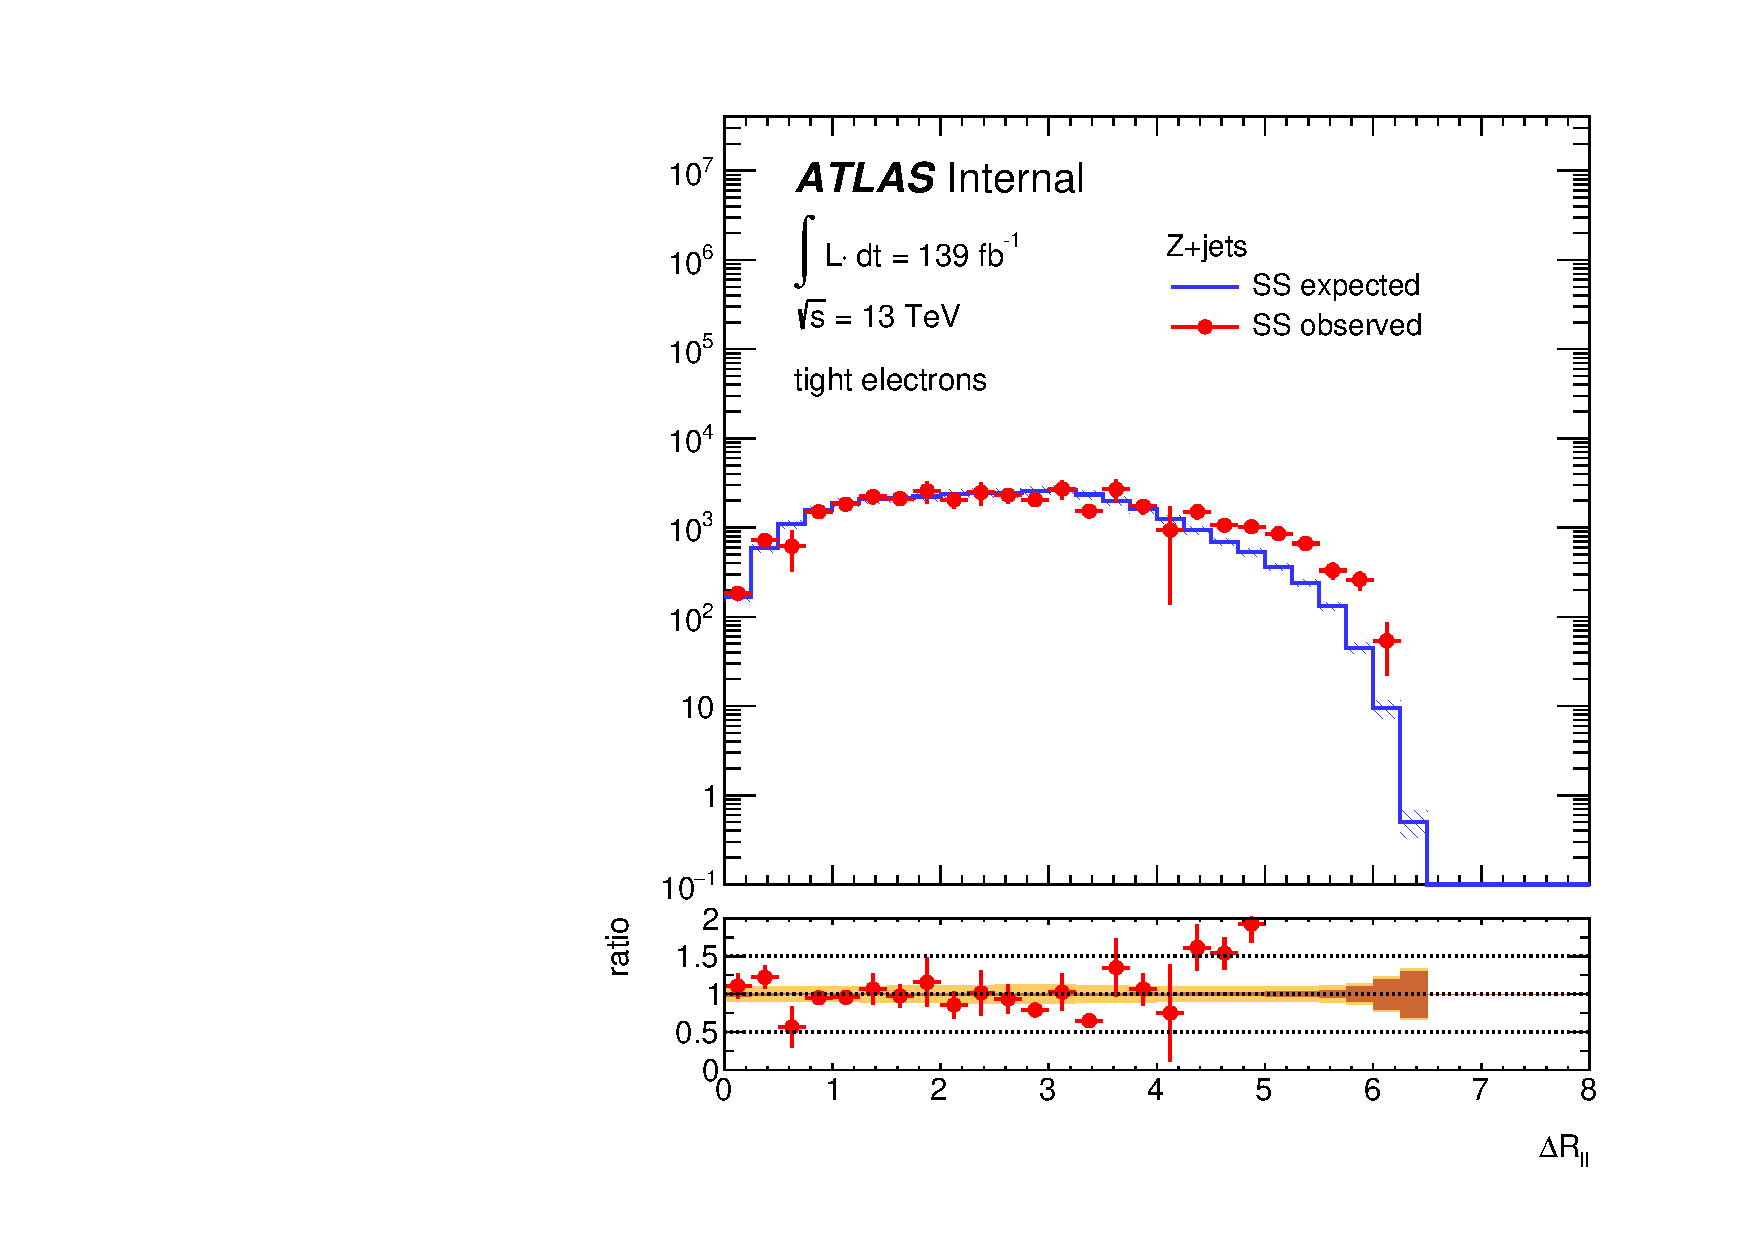
\includegraphics[width=0.45\textwidth]{figures/qmisid/valid_DRlltightZ}\\
  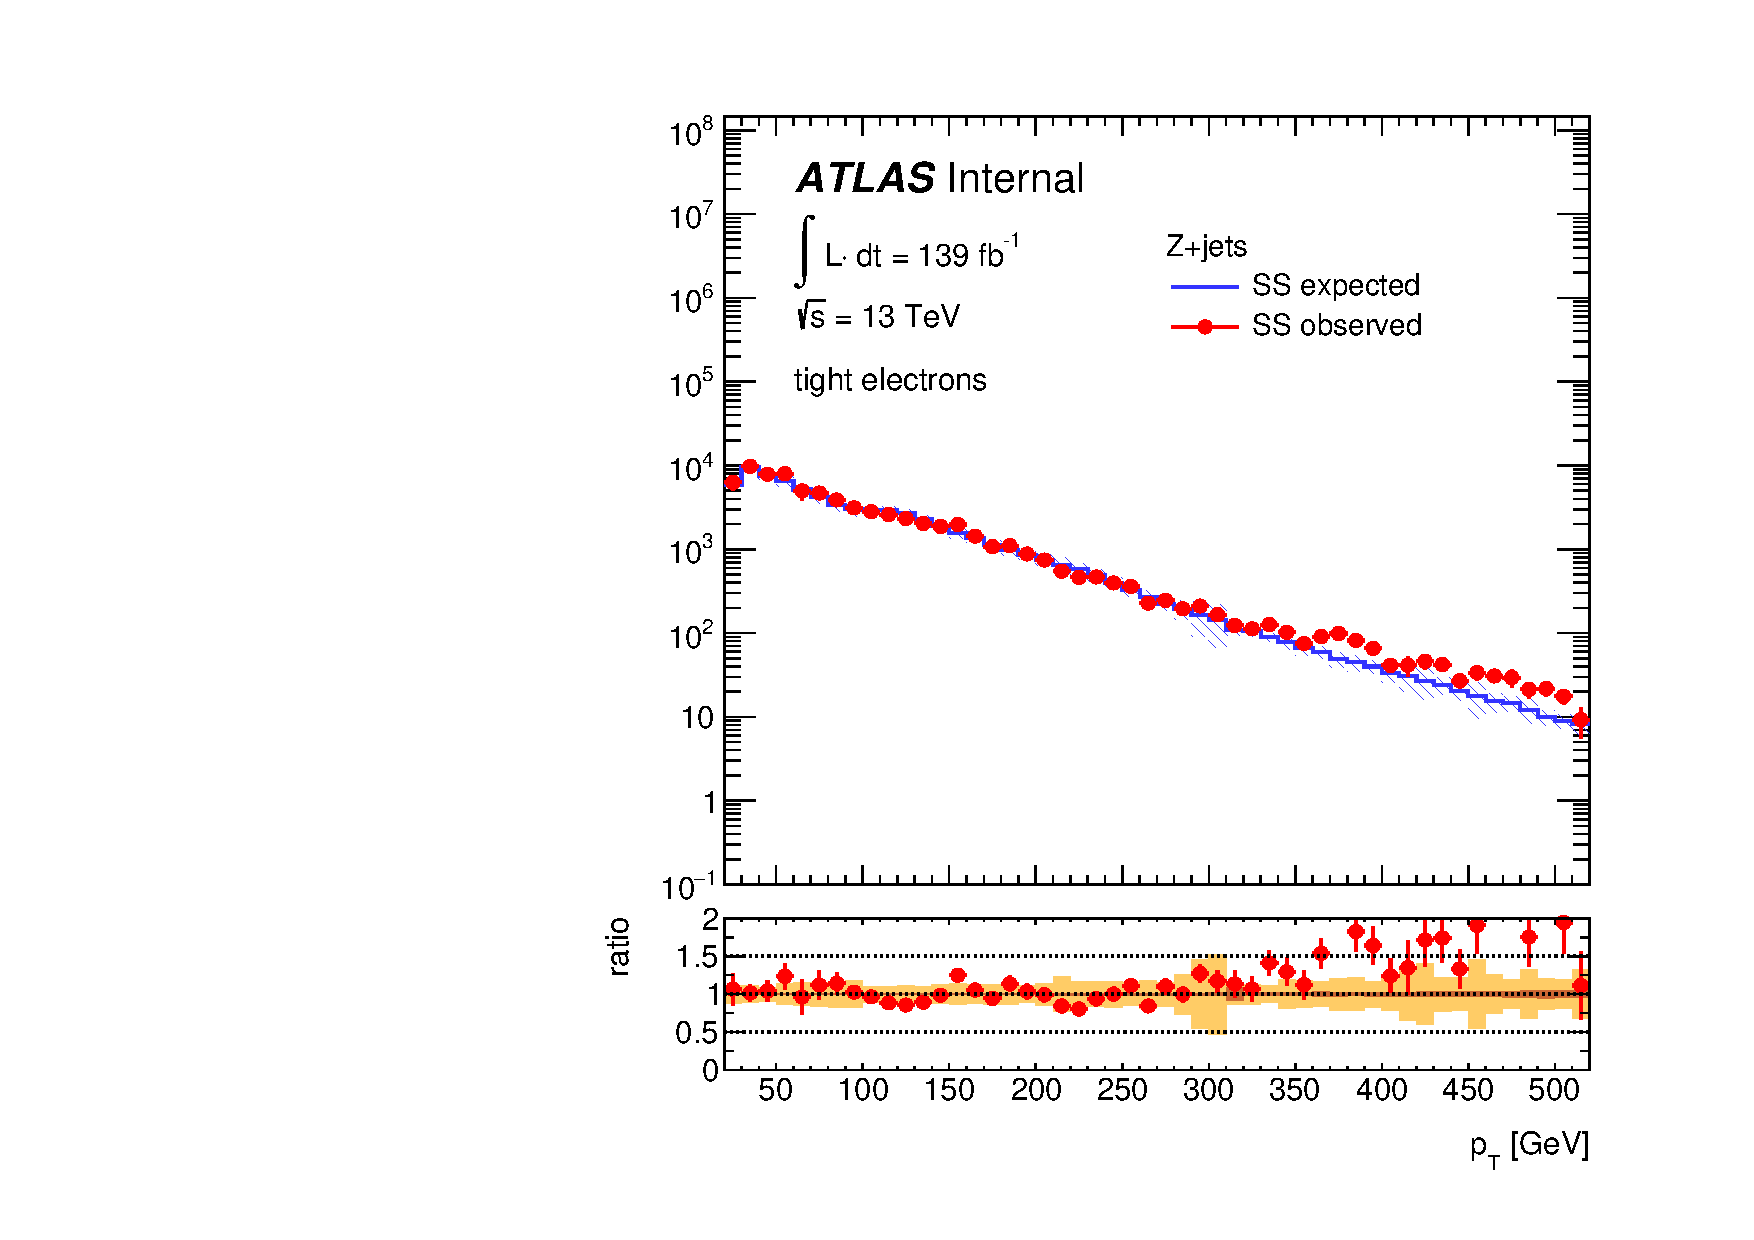
\includegraphics[width=0.45\textwidth]{figures/qmisid/valid_PttightZ}
  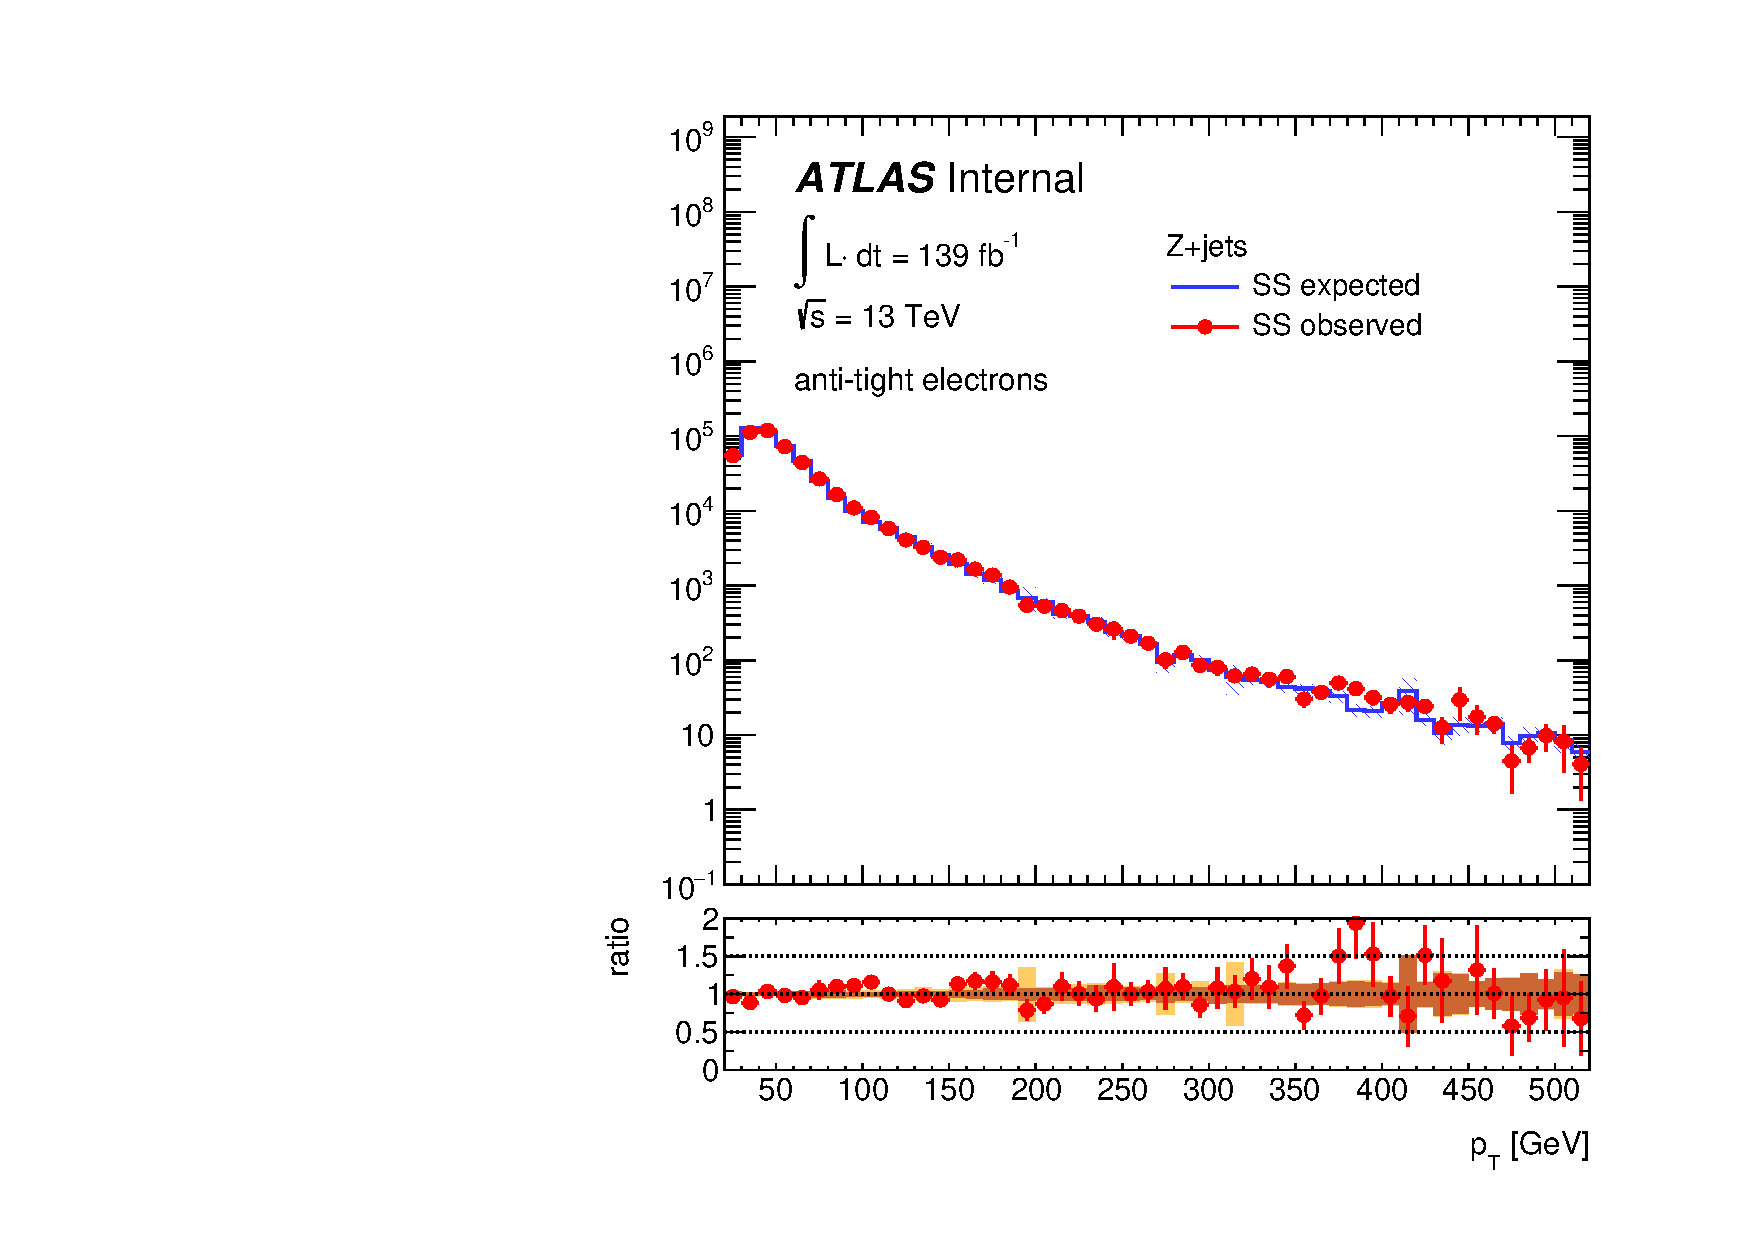
\includegraphics[width=0.45\textwidth]{figures/qmisid/valid_PtatightZ}\\
  \caption{Comparison between the expected and observed $m_{ee}$,
${\Delta}R_{ee}$, $\pT$ (tight) and $\pT$ (anti-tight) of same-sign electrons.
The dashed bands represent the total (statistical + systematic) uncertainty of the estimation.
 The comparison is shown for $Z$+jets events. Fake electrons are removed from
 the sample by using the truth information.\label{fig:clMC}} 
\end{figure}

Tables and Plots need to be updated.
\subsection{Lepton definition}
The selection of lepton use the official working point of identification and isolation. All baseline leptons are classified into the tight and loose category, the loose leptons are used for fake background estimation. The way to choose the optimized working point is to scan the significance from a set of possible combinations.\\

Electrons are reconstructed by matching the energy deposits from the EM calorimrter to the track in the inner detector. LHLoose and LHTight identification working point are used for loose and tight electron respectively. They are required to have $p_T$>20\GeV and $|\eta|<2.5$, the electron within the transition region between barrel and endcap electromagnetic calorimeter, $1.37<|\eta|<1.52$ are vetoed. To reduce the non-prompt electron contribution, cuts on the transverse parameter significance $d_0$ and longitudinal impact parameter $Z_0$ are applied to ensure that the electron originates from a primary vertex.\\
Muons are reconstructed by using the information of Muon spectrometer and the Inner detector. Muon candidates are selected with $p_T>20GeV$ and $|\eta|<2.5$. They are required to pass the Loose and Medium identification workinf point for loose and tight muons. The impact parameter cut remain the same as electron but transverse parameter significance cut is more tight than electrons.\\
Further tight selections are required to supress non-prompt and fake background entering into signal region. PLVTight, recommended by the Isolation and Fake Forum group, is applied. In addition, electrons candidates should pass a charge misidentification BDT working point to reduce charge flip background contribution. Furthermore, the photon conversion background is not negligible in this analysis, electrons are required to fullfill the ambiguity bit selection.\\
The lepton definition of loose and tight categories are summarized in Table\ref{tab:lepton_selection}.
\begin{table}[h!]
 \begin{center}
   \begin{tabular}{cc}
     \toprule
              &  \\
     \midrule
      $\mu$              & \verb!HLT_mu26_ivarmedium, HLT_mu50!	\\
     \multirow{2}*{$e$}  & \verb!HLT_e26_lhtight_nod0_ivarloose, HLT_e60_lhmedium_nod0,! \\
                         & \verb!HLT_e140_lhloose_nod0!	\\
     \bottomrule
   \end{tabular}
   \caption{\label{tab:lepton_selection}}
 \end{center}
\end{table}


\subsection{Event selection}
\label{sec:EventSelection}
The same charged leptons events are split into three channels according to the lepton flavors: $e^{\pm}e^{\pm}$,$\mu^{\pm}\mu^{\pm}$ and $e^{\pm}\mu^{\pm}$. The two leptons are required to pass tight lepton requirement listed in Table. Both letptons must satisfy transverse momentum $p_T>20GeV$ and their invariant mass $m_{ll}>15GeV$.An dditional invariant mass Z-veto is applied for two electrons channel only to remove charge mis-identification(QmisID) events. There must be no $\tau_had$ candidates in the event. Events must have at least 3 jet and no b-jet with $70\%$ b-tagging efficiency. 
The cutflow for non resonant signal, $VV$ , $ttbar$ and $Wjets$ processes are presented in Table.	
\subsection{Background estimation}
After pre-selection the background source for 2LSS channel can be classified into to two categories. The irreducible background are events where all candidates are prompt leptons or are decayed from $\tau$. The reducible background where events at least one of the candidate leptons is not a prompt lepton consists of charge misidentified leptons and fake leptons. In the first category, the prompt leptons are mainly from diboson process, $WZ,W^{\pm}W^{\pm}$, $tV,ttV,t\bar{t}H$ and $VH$, where $V$ stands for $W$ or $Z$ bosons. Those ingredient are illustrated in Figure, the discrepancy between data and pure MC simulation indicates that QmisID and fakes leptons are not well modeled by MC, so data-driven estimations are needed to describle this two background.

\subsubsection{Charge mis-identified background}

For the SS2L channel, prompt background events from Z+jets and $t\bar{t}$ with two opposite-charge same flavour leptons can pass tight selection due to charge flip. The misidentification of the muon charge-sign is not considered in this study, because the track curvature are measured with the help of muon spectrometer resulting in negligible muuon QmisID rate, generally below $10^{-5}$.\\
There are two sources contributing to electron QmisID. The most likely mechanism of electron QmisID is hard Bremsstrahlung process ($e^{\pm} \rightarrow e^{\pm} \gamma^{*} \rightarrow e^{\pm} e^{+} e^{-}$). When an electron emits bremsssstrahlung, then the radiated photon converts into $e^+e^-$ pair because of interations with detector material. The energy deposits in the calorimeters may be reconstructed by matching the track of the opposite-sign electron. Since the Bremsstrahlung process depends on the amount of traversed detector material, the $|\eta|$ dependence on the QmisID rate would be considered. Charge fliped events could also arise from measurement error of the electron track curvature. This effect is more significant for electrons with high momenta or at large pesudorapidites, thus the $p_T$ dependence would also be considered.\\
The MC simulation on QmisID are not fully realiable due to the complicated processes with detector materials. The QmisID rates  are esimated using a data-driven method based on a maximum likelihood technique. The likelihood fit is done on $Z ->ee$ data sample, events around $Z$ peak are categorized into same-sign electron pair(SS) or opposite-sign pair(OS). The contribution from other small background are subtracted from the side-band data. The number of same-sign electron pair ($N_{SS}$) and number of opposite-sign electron pair($N_{OS}$) are the input of this fit. The probability to observe same-sign pairs follows a Possion statistic, write as 
\begin{equation}
f\left(N_{\mathrm{SS}}^{i j} ; \hat{N}_{\mathrm{SS}}^{i j}\left(\varepsilon_{i}, \varepsilon_{j}\right)\right)=\frac{\lambda^{N_{\mathrm{SS}}^{i j}} \mathrm{e}^{-\hat{N}_{\mathrm{SS}}^{i j}\left(\varepsilon_{i}, \varepsilon_{j}\right)}}{N_{\mathrm{SS}}^{i j} !}
\end{equation}

Where $\varepsilon_{i}$ and $\varepsilon_{j}$ represent the QmisID rates for each of two electrons in bin$(i,j)$, $N_SC^{i j}$ is the number of same-sign pairs,$\hat{N}_{\mathrm{SS}}^{i j}\left(\varepsilon_{i}, \varepsilon_{j}\right) = N^{ij}(\varepsilon_{i}(1-\varepsilon_{j})+\varepsilon_{j}(1-\varepsilon_{i}))$ is the expected number of same-sign events. The expected number of QmisID events $\hat{N}_{\mathrm{SS}}^{i j}\left(\varepsilon_{i}, \varepsilon_{j}\right)$ therefor can be computed by measuring the number of opposite-sign events $N_{OS}$ and QmisID rates in $e^{\pm}e^{\pm}$ and $e^{\pm}\mu^{\pm}$ channels,
\begin{equation}
\hat{N}_{\mathrm{SS}}=\frac{\varepsilon_{i}+\varepsilon_{j}-2 \varepsilon_{i} \varepsilon_{j}}{1-\left(\varepsilon_{i}+\varepsilon_{j}-2 \varepsilon_{i} \varepsilon_{j}\right)} N_{\mathrm{OS}} \quad \text { and } \quad \hat{N}_{\mathrm{SS}}=\frac{\varepsilon_{i}}{1-\varepsilon_{i}} N_{\mathrm{OS}}
\end{equation}

The negative log likelihood used to determine the QmisID rates is constructed as 
\begin{equation}
-\ln L\left(\varepsilon \mid N_{S S}, N\right)=\sum_{i, j} \ln \left[N^{i j}\left(\varepsilon_{i}(1-\varepsilon_{j})+\varepsilon_{j}(1- \varepsilon_{i})\right)\right] N_{S S}^{i j}-N^{i j}\left(\varepsilon_{i}(1-\varepsilon_{j})+\varepsilon_{j}(1- \varepsilon_{i})\right)
 \end{equation}
The QmiID rate are parameterized as a function of electron $p_T$ and $|\eta|$. The binnings scheme are designed as [10,60],[60,90],[90,130],[130,1000] in electron $p_T$ and [0,0.6],[0.6,1.1],[1.1,1.37][1.52,1.7],[1.7,2],[2,2.5]. The events are required that two tight leptons pass pre-selection with an invariant mass window, the Z-peak is obtained by a Gaussian fit, then $\pm4\sigma$ around the mean value is defined as the $m_Z$ window. In terms of background subtraction the side-bands region are defined by $\pm4\sigma$ width for each side of $m_Z$ window. Since the invariant mass spectra of two same-sign electrons is shifted comparing with opposite-sign electrons, the $m_Z$ window and side-bands are used differently for this two case. To increse the statistic of the tight-electrons, anti-tight electrons are tested in this estimation. As shown in Figure \ref{fig:qmisid_mll}, no significant difference is found for different combinition of tight and an-tight electron pairs. From the fit the definitions of the $m_Z$ window are listed in table
%\begin{figure}[!htb]
%\centering
%\subfigure[]{\includegraphics[width=0.4\textwidth]{figures/}}
%\subfigure[]{\includegraphics[width=0.4\textwidth]{figures/}}
%\quad 
%\subfigure[]{\includegraphics[width=0.4\textwidth]{figures/}}
%\subfigure[]{\includegraphics[width=0.4\textwidth]{figures/}}
%\caption{
%}
%\label{fig:qmisid_mll}
%\end{figure}

To validate the likelihood method used to determine QmisID rates, a closure test is done by comparing the QmisID rates derived from Z+jets simulation with the rates using truth information. There is no big disagreement between the two approaches, as the comparion plots shown in figure.


Three sources of systematic uncertainties are considered for QmisID background esimation:
\begin{itemize}
\item The statistical uncertainty in each $p_T-\eta$ bins due to the statistial size of data site in control regions.
\item The difference between the rates measured by likelihood method and the rates derieved from truth matched method.
\item Background subtraction uncertainties. The variation of the rates with the definition of the $m_Z$ window by 1 $\sigma$ difference is regarded as uncertainty.
\end{itemize}

\subsubsection{Non-prompt lepton background}{}

The fake leptons are important background in 2LSS channel. Events originate from non-prompt and fake backgrounds can also contribute to same-sign lepton final state. In this document non-prompt and fake leptons form the fake background. There are several sources of non-prompt and fake leptons.\\
	Non-prompt leptons arise mainly from  heavy flavor decays, they are real leptons but not produced from primary interaction point. In addition to non-prompt leptons, hadronic jet are misidentified as prompt charged leptons, lectrons from photon conversion, making the fake leptons consist of multiple components.\\ 
	Simulating each process which leads to a fake lepton is not reliable and precise in MC samples, leading to a challenging estimation on fake background. For this reason, data-driven method is necessary to make a reasonable fake estmation. In this analysis, $t\bar{t}$  and $W+jets$ are main processes providing fake lepton. The fake factor method is used to discribe fake lepton background, both two leptons originating from fakes are not considered yet.\\
	The number of prompt leptons is esitmated using both data and MC simulation on a fake en-riched control region. The control region is constructed by same-sign events in which one lepton pass the tight selection and another lepton so-called anti-tight lepton fails the tight selection. In this method, two fake factors ralated the events from fake en-riched region to the background in signal region are derieved. The method assumes that the fake factor is independent of jet multiplicity. The fake factor is defined as the ratio of number of same-sign events with two tight leptons between same-sign events with one tight lepton and one anti-tight lepton, as below
\begin{equation}
\theta_{\ell}=\frac{N_{\ell \ell}}{N_{\ell \ell}}
\end{equation}
where $\ell$ the tight lepton e or $\mu$ and $\ell$ the anti-tight lepton e or $\mu$. In the signal region, the fake electrons are dominated by jets misidentified as electrons, following the photon conversions and non-prompt heavy flavour decay products. A check on fake lepton componsion is preformed in low jet multiplicity and high jet multiplicity region. The fake componsion, consist of External Conversion, internal conversion, b decay, c or other decay, and rest unknown, are classified by TruthClassifier Tool. A non QmisID origination selection is required to avoid the contamination from charge fliped electrons. Fake composition	looks similar for low jet multiplicity control region and high jet multiplicity signal region.

The fake factors for $\ell$ and $\mu$ can be written as 
\begin{equation}
\theta_{e}\left(1 \leq N_{\text {jet }} \leq 2\right)=\frac{N_{e e}^{\text {data }}-N_{e e}^{\text {prompt }}-N_{e e}^{V \gamma}-N_{e e}^{\text {QmisID }}}{N_{e \phi}^{\text {data }}-N_{e \phi}^{\text {prompt }}-N_{e \phi}^{V \gamma}-N_{e \phi}^{\text {QmisID MC }}}
\end{equation}

\begin{equation}
\theta_{e}\left(1 \leq N_{\text {jet }} \leq 2\right)=\frac{N_{e e}^{\text {data }}-N_{e e}^{\text {prompt }}-N_{e e}^{V \gamma}-N_{e e}^{\text {QmisID }}}{N_{e \phi}^{\text {data }}-N_{e \phi}^{\text {prompt }}-N_{e \phi}^{V \gamma}-N_{e \phi}^{\text {QmisID MC }}}
\end{equation}

In both denominator and numerator region, the contributions from other background, composed of prompt same-sign leptons from VV,VVV,VH,tV,ttV and ttH processes, V$\gam$ process and QmisID process, are subtracted. $N^{prompt}$ the  background from prompt sames-sign lepton pair and V$\gam$ backgound are estimated using MC simulation. For fake factor of electron, $N^{QmisID}$ in the numerator is estimated from opposite-sign events computing with correspondingQmisID rates as discussed in section. In the denominator, $N^{QmisID}$ is computed from MC events in which one electron is required to be a real electron.\\

The fake factors are measured in a control region. A b-veto is applied to suppress fakes from $t\bar{t}$ events. Due to the fact that the sub-leading lepton is an anti-tight lepton in most cases, thus for numberator events, the sub-leading lepton is chosen to be the fake candidate. While for one tight lepton and one anti-tight lrpton in denominator, no subleading lepton should match to anti-tight selection. It was found that an inclusive fake factor can't describle the distribution of lepton kinematics, $\eta$, $\pt$ very well. A $p_T$ dependence fake factor therefore is raised to be implemented in each $p_T$ bins. The $p_T$ are divided into 4 bins, [20,40],[40,60],[60,100],[100,1000]. The $\eta$ and $p_T$ dependent fake factor is presented in figure.\\

Note: the result is based on $p_T$ dependent fake factor only, will update to $|\eta|-pt$ 2D-space fakes estimationlater.\\
Each kinds of subtracted background and observed data in low jet multiplicity region is listed in Table and Table for electrons and muons. To measure the number of fakes in signal region, following equations are used,

\begin{equation}
N_{e e}^{\text {fakes }}\left(N_{\text {jet }} \geq 3\right)=\left(N_{e \phi}^{\text {data }}-N_{e \phi}^{\text {promptSS }}-N_{e \phi}^{V \gamma}-N_{e \phi}^{\text {QmisID MC }}\right)\left(N_{\text {jet }} \geq 3\right) \times \theta_{e}
\end{equation}

\begin{equation}
N_{\mu \mu}^{\text {fakes }}\left(N_{\text {jet }} \geq 3\right)=\left(N_{\mu \mu}^{\text {data }}-N_{\mu \mu}^{\text {promptSS }}-N_{\mu \not h}^{V \gamma}\right)\left(N_{\text {jet }} \geq 3\right) \times \theta_{\mu}
\end{equation}

\begin{equation}
\begin{aligned}
N_{e \mu}^{\text {fakes }}\left(N_{\text {jet }} \geq 3\right.&)=\left(N_{e \mu}-N_{e \mu}^{\text {promptSS }}-N_{e \mu^{\mu}}^{V \gamma}-N_{e \mu}^{\text {QmisID }}\right)\left(N_{\text {jet }} \geq 3\right) \times \theta_{\mu} \\
	+&\left(N_{\phi \mu}-N_{\phi \mu}^{\text {promptSS }}-N_{\phi \mu}^{V \gamma}-N_{\phi \mu}^{\text {QmisID MC }}\right)\left(N_{\text {jet }} \geq 3\right) \times \theta_{e}
\end{aligned}
\end{equation}

The number of predicted fakes after pre-selections in $N_{jet}==3$ region is shown in table, the uncertainties hereare stat-only. 
\subsubsection{Fake background systematics uncertainties}
Following sources of systematic uncertainties on estimated fake factors are presented

\begin{itemize}
\item The statistical uncertainty on fake factors $\theta_e$ and $\theta_{\mu}$. 
\item The uncertainty of QmisID estimation: the full uncertainty on this background is propagated to the fake factor measuremnet.
\item The systematics on MC modeling 
\item The uncertainty on jet multiplicity extrapolation: the fake factor is measured from low jet multiplicity region and is applyed in high jet multiplicity region. The assumption of a stable fake factor with respect to $N_jet$ may not always true. To take this difference into account the fake from MC(require two tight lepton in ttbar samples) are compared with the fakes estimated by fake factor method. 
\item sample dependence
\end{itemize}
\subsection{Background validation}
By means of data-driven method the QmisID, fake background and irreducible background are compared with the number of observed data in figure. The event yield at pre-selection level is presented in table for different flavor channels. In general a good agreement is observed between data and total estimated backgrounds within uncertainties, 

\subsection{Signal optimization}
\subsection{Signal topology}

The signal of 2LSS channel consist of two same sign leptons, with multiple jets and $E_T^{miss}$. From the truth level kinematics distribution of di-higgs, this two higgs bosons tends to flight in the opposite direction, as shown in figure. Afterwards two higgs bosons decay to W-W pair, Z-Z pair or tau-tau pair indenpendently. Thus it's challenging to separate multiple signals with different kinematic properties, classification work preformed by multivariate analysis technique are motivated to improve analysis sensitively.\\


\subsection{Signal region using MVA}


The following varibles are used for MVA optimization process.\\
\begin{itemize}
\item $M_l1j$ invariant mass of leading lepton and its clostest jet
\item $M_21j$ invariant mass of sub-leading lepton and its clostest jet
\item $\Delta R(l_0,j)$ $\Delta R$ distance of leading lepton and its clostest jet
\item $\Delta R(l_1,j)$ $\Delta R$ distance of sub-leading lepton and its clostest jet
\item $m_ll$ invariant mass of two same-sign leptons.
\item $m_{all}$ invariant mass of all selected objects.
\item $\eta$ of two leptons, $\eta_{l0},\eta_{l1},max(\eta_{l1},\eta_{l2}),$ 
\item $\Delta R(l0,l1)$ $\Delta R$ distance of two same-sign leptons.
\item HT the scalar sum of $p_T$ of all object. 
\item three lepton channels with different flavour, $e^{\pm}e^{\pm,\mu^{\pm}\mu^{\pm},e^{\pm}\mu^{\pm}}$
\item number of jet.
\item $p_T$ of subleading jet
\end{itemize}

The input variables that have the highest separation power are listed in Table\ref{tab:separation_power} \\
\begin{table}[h!]
 \begin{center}
   \begin{tabular}{cc}
     \toprule
              &  \\
     \midrule
      $m_l1j$              & 2.13e-1\\
     \midrule       
      $mindR_l1j$          & 1.78e-1\\
     \midrule       
      $mindR_l1j$          & 1.78e-1\\
     \midrule       
      $mindR_l1j$          & 1.78e-1\\
     \midrule       
      $mindR_l1j$          & 1.78e-1\\
     \midrule       
      $mindR_l1j$          & 1.78e-1\\
     \midrule       
      $mindR_l1j$          & 1.78e-1\\
     \midrule       
      $mindR_l1j$          & 1.78e-1\\
     \midrule       
      $mindR_l1j$         & 1.78e-1\\
     \midrule       
      $mindR_l1j$          & 1.78e-1\\
     \bottomrule
   \end{tabular}
   \caption{\label{tab:separation_power}}
 \end{center}
\end{table}
Figure show the distributions of the input variables for signal and estimated background where QmisID and fake leptons are modelled by data-driven methods discussed in previous section\\

Before the training procedure a comparsion of fakes simulated by ttbar and W+jet MC(MC fakes), with fakes estimated by fake factor method(DD fakes) is preformed. The motivation of this check is to avoid problematic negetive events weight during training. The shape distrbution for main discriminate varibles are presented in Figure. Generally the agreement is good expect seveal bins contaning big weight of W+jets events. The scale factor of normalizing MC fakes yields to DD yields is found to be 0.974.\\
Signal samples are events within two tight leptons pass all events selection, the background samples includes the main background, $VV$, $ttbar$ and $Vjet$. Signal and background BDTG response distributions for training and test are shown in Figure. The agreement between the two shape indicates that there is no overtraining.\\

The training model is applied to signal samples and full background samples where QmisID and fake leptons are estimated by data-driven method. The BDTG dicrimination in Figure illustrates that the signal and background events are well separated to two sides.\\
By scaning the BDTG distribution, it is found that BDTG cut at 0.78 gives 0.058 significance in maximum. Considering the BDTG sc as observeble, 
\subsection{Results}
The Statistical interpretations are preformed by TRexFitter. The input event yields is listed in Table

\subsection{2$\ell \ell$SS - MVA V2}

%\subsubsection{The strategy}
In order to define Signal Region, a BDT has been trained. In this MVA
approach, the strategy is to train 3 specific BDTs, targetting the 3 main
background processes. In the 2$\mathrm{\ell \ell}$SS channel, these
backgrounds correspond to diboson, V+jets and ttbar
productions. Various discriminating 
variables are used according the targetted background process. Then, the 3 BDT
outputs are combined into a final discriminant variable using a fourth
BDT. For each training (of the specific BDTs or the combined one) the MVA
method is the BDTG. 
While the combined BDT is used to define the signal region, the
background specific BDTs can be used to defined background enriched
regions (Validation Regions and potential Control Regions) targetting
the 3 leading background seperately.  

\subsubsection{Selections and leptons definition}
Some preselections have been applied: 
\begin{itemize}
    \item 2LSS: 2 leptons same sign
    \item $\tau$ and bjets VETOS
    \item 2 $\leq$ Number of jets $\leq$ 7
    \item Invariant mass of the 2 leptons $\geq$ 12~GeV
\end{itemize}
Then the leptons have been defined as: 
\begin{itemize}
    \item Tight ID for electrons
    \item Medium ID for muons
    \item Transversal momentum $\geq$ 20~GeV
    \item $\eta$ $\leq$ 2 for electrons
    \item Prompt lepton veto tight for electrons and muons
    \item QIDBDT $\geq$ -0.3
\end{itemize}
Finally some selections about the trigger decision have been applied, knowing Global Trig decision and Cust Trig match Single Lepton Trigger or Di-Leptons Trigger and the associated Scale Factors. 

\subsubsection{Discriminating variables}
The variables used as inputs to the various MVAs are listed in the following:
\begin{itemize}
    \item $M_{\ell \ell}$: the invariant mass of the di-leptonic system
    \item $M_{all}$: the invariant mass of all selected objects
    \item $M_{\ell0 j}$: the invariant mass of the leading and its closest jet
    \item $M_{\ell1 j}$: the invariant mass of the subleading and its closest jet
    \item $M_{W0}^T and M_{W1}^T$: the W transverse mass using the
      leading and the subleading leptons.
    \item MET : Missing transverse energy 
    \item $\eta_0$ and $\eta_1$: $\eta$ of the leading and the subleading leptons
    \item $\Delta \eta$: absolute value of $\eta_0$-$\eta_1$
    \item Number of jets
    \item Number of b-tagged jets at a 85\% efficiency: It has
      been only used for the BDT training specific to ttbar
      background. In fact, the decay of ttbar will induce a b-quark
      emission. 
      This input will be discarded in the futur due to the complexity of
      using a continous Btagging in association to the b-veto at 77\%
      applied at the preselection level
    \item HT: Scalar sum of transversal impulsion for all objects
    \item $HT_{lep}$: Scalar sum of transversal momentum for leptons
    \item Dilep\_type: =1 if $\mu \mu$, =2 if $e\mu$ or $\mu e$, =3 if ee
    \item $\Delta R _{min \ell0 jets}$: Minimum distance between the leading lepton and its closest jet
    \item $\Delta R _{min \ell1 jets}$: Minimum distance between the subleading lepton and its closest jet
    \item $\Delta R _{\ell \ell}$: Distance between the leading and the subleading leptons
    \item Total\_charge: Sum of the charge of the leading and the
      subleading lepton. The total charge is specific to the VV
      BDT. In the 2LSS, VV background is mainly due to WZ events.
     Unlike the HH final state, a charge asymetry is therefore
     expected in the VV final state (As shown in
     Figure~\ref{fig:totQ_distri_2LSS}).  
\end{itemize}

\begin{figure}[!h]
    \centering
    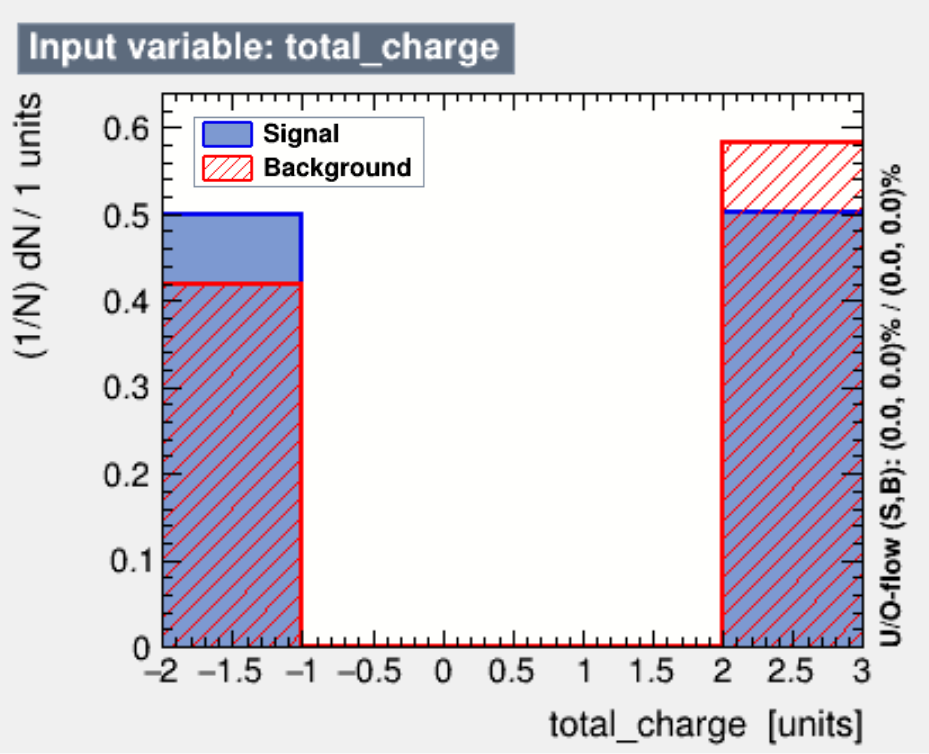
\includegraphics[width=0.5\textwidth]{figures/2LSS/totQ_distri.png}
    \caption{Total charge distribution with training selection}
    \label{fig:totQ_distri_2LSS}
\end{figure}
 
\subsubsection{Specific BDTs}
The 3 specific BDTs have been trained with the following parameters: 
\begin{itemize}
    \item VV vs HH training: 17 variables have been used as input variables. 14,289 events and 300,000 events have been used respectively for signal and diboson background. 
    \item Vjets vs HH training: 16 variables have been used as input variables. 15,000 events and 15,000 events have been used respectively for signal and V+jets background.
    \item $\mathrm{t\bar{t}}$ vs HH training: 17 variables have been used as input variables. 14,289 events and 2,900 events have been used respectively for signal and $\mathrm{t\bar{t}}$  background.
\end{itemize}
Figures \ref{fig:VV_BDT}, \ref{fig:tt_BDT} and \ref{fig:Vjets_BDT} show the distribution of each resulting output.

\begin{figure}[!h]
\begin{minipage}[c]{.5\linewidth}
    \centering
  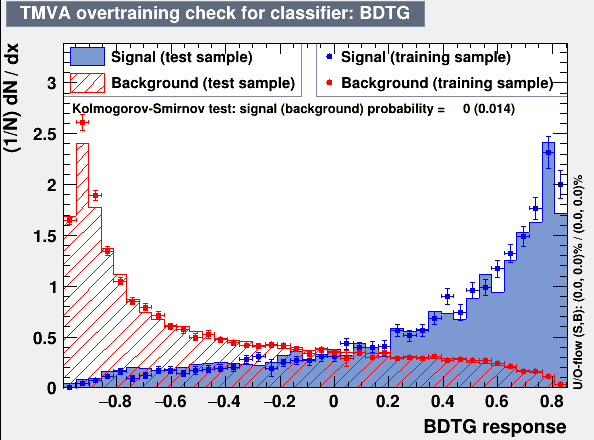
\includegraphics[width=\textwidth]{figures/2LSS/VV_BDT.png}
  \caption{Discriminant output of VV VS HH training}
  \label{fig:VV_BDT}
\end{minipage}
\begin{minipage}[c]{.5\linewidth}
  \centering
  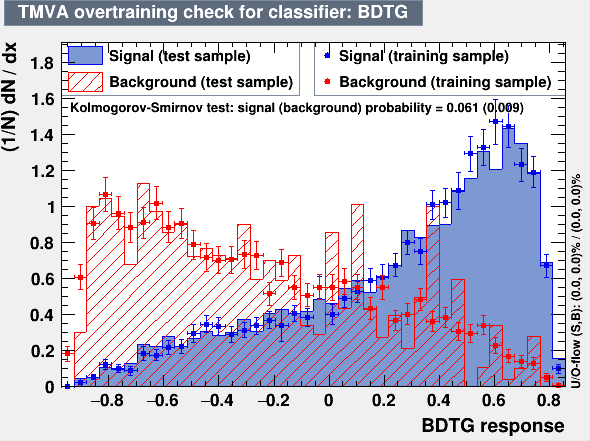
\includegraphics[width=\textwidth]{figures/2LSS/tt_BDT.png}
  \caption{Discriminant output of $\mathrm{t\bar{t}}$ VS HH training}
  \label{fig:tt_BDT}
\end{minipage}
\begin{minipage}[c]{\linewidth} 
  \centering
  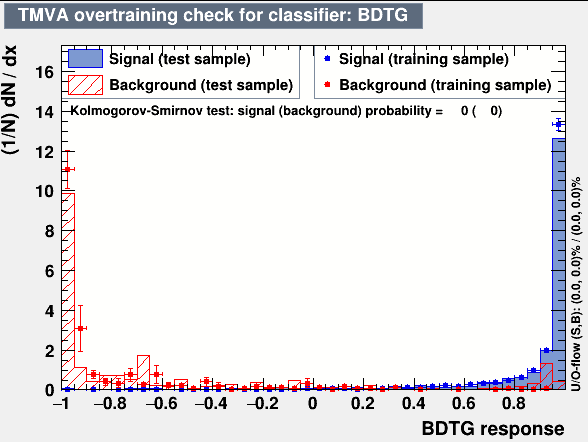
\includegraphics[width=.5\textwidth]{figures/2LSS/Vjets_BDT.png}
  \caption{Discriminant output of V+jets VS HH training}
  \label{fig:Vjets_BDT}
\end{minipage}
\end{figure}

\subsubsection{The Combined BDT}
Then, a new final discriminating variable was obtained by training a
new BDT that combines the 3 previous specific BDTs. For the training,
only the 3 main backgrounds were considered, using the MC
simulation. The 3 specific BDTs have been chosen as input variables,
14,289 events and 317,900 events was considered repectivelly for
signal and backgrounds. The final discriminant is shown on Figure~\ref{fig:BDT}.\\  
Finally, in order to quantify the sensitivity of the signal region
defined by this MVA, a full fit has been performed using TRExFitter,
including all the MC based backgrounds. The fit of the Asimov dataset
leads  to a limit $\mu_{95\%}$ equals to 29.9 (stat only) using 
the BDT shape.
As a cross-check, considering the invariant mass shape
(cf. Figure~\ref{fig:Mll_BDT}) and applying a selection on the BDT
(BDT $\geq$ 0.787), the limit has been settled at 34.6 (stat only).

\begin{figure}[!h]
\begin{minipage}[c]{.5\linewidth}
  \centering
  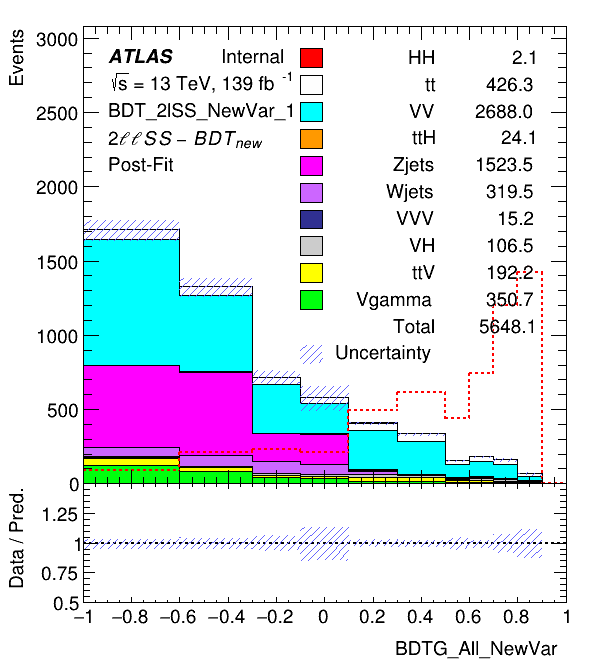
\includegraphics[width=\textwidth]{figures/2LSS/HH_l20tau_NewDef2.png}
  \caption{Final BDT distribution}
  \label{fig:BDT}
\end{minipage}
\begin{minipage}[c]{.5\linewidth}
    \centering
    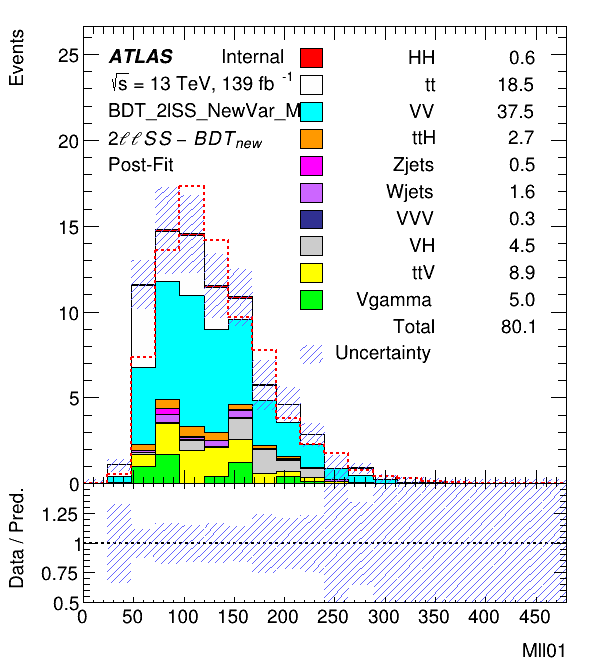
\includegraphics[width=\textwidth]{figures/2LSS/HH_l20tau_NewDef_postFit.png}
    \caption{Mll distribution, BDT $\geq$ 0.787}
    \label{fig:Mll_BDT}
\end{minipage}
\end{figure}
